\chapter{
Beyond SBDRL I: global algebras
(V1.0)
}

%%%%%%%%%%%%%%%%%%%%%%%%%%%%%%%%%%%%%%%%%%%%%
\section{What about walls ?}

Let's take our $2 \times 2$ cyclic grid world $\mathscr{W}_{\alpha}$ and add a wall to give a new world $\mathscr{W}_{\beta}$.

\begin{figure}[H]
  \centering
    \begin{subfigure}[b]{0.45\linewidth}
        \centering
        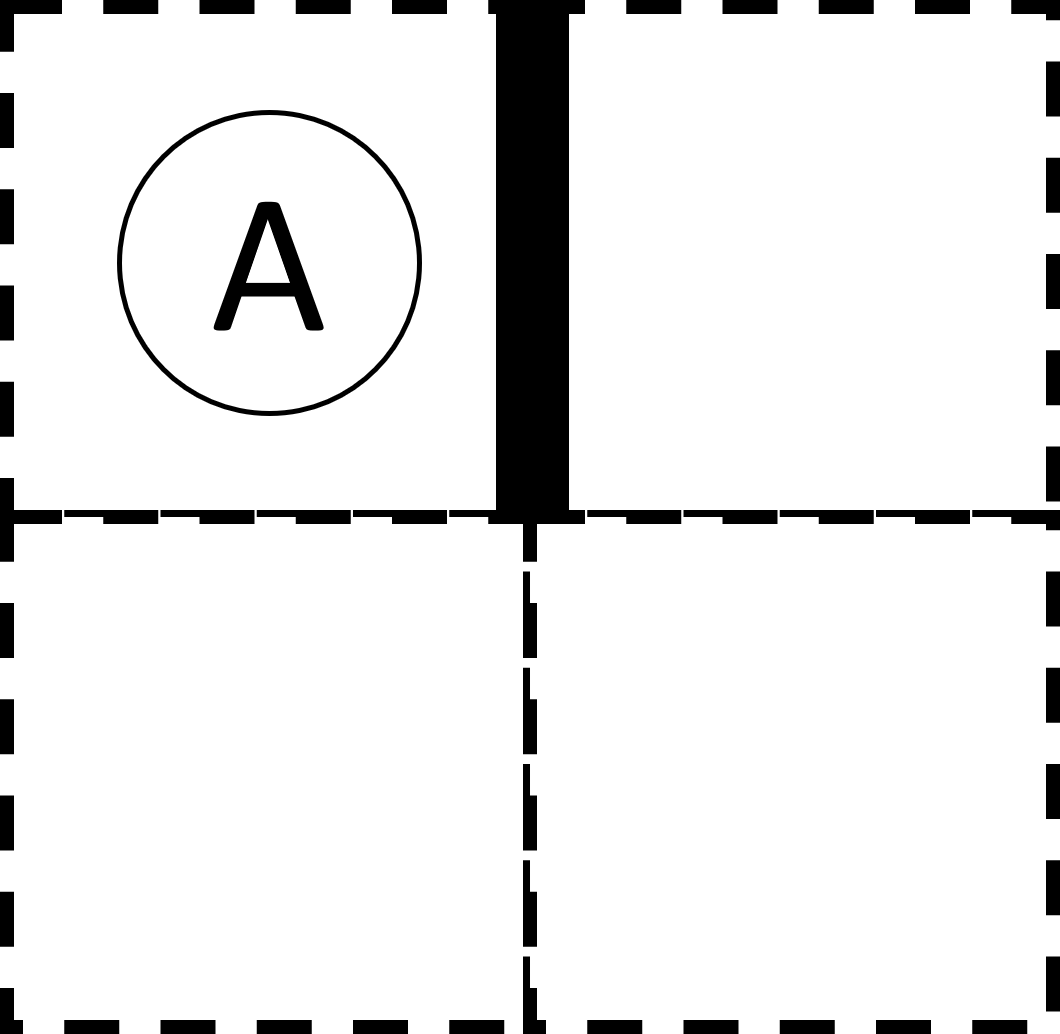
\includegraphics[width=0.5\linewidth]{5BeyondSBDRLGlobalAlgebras/Images/2x2_with_wall_world_states/w0.png}
        \caption{$w_{0}$}
        \vspace{0.25cm}
    \end{subfigure}
    \begin{subfigure}[b]{0.45\linewidth}
        \centering
        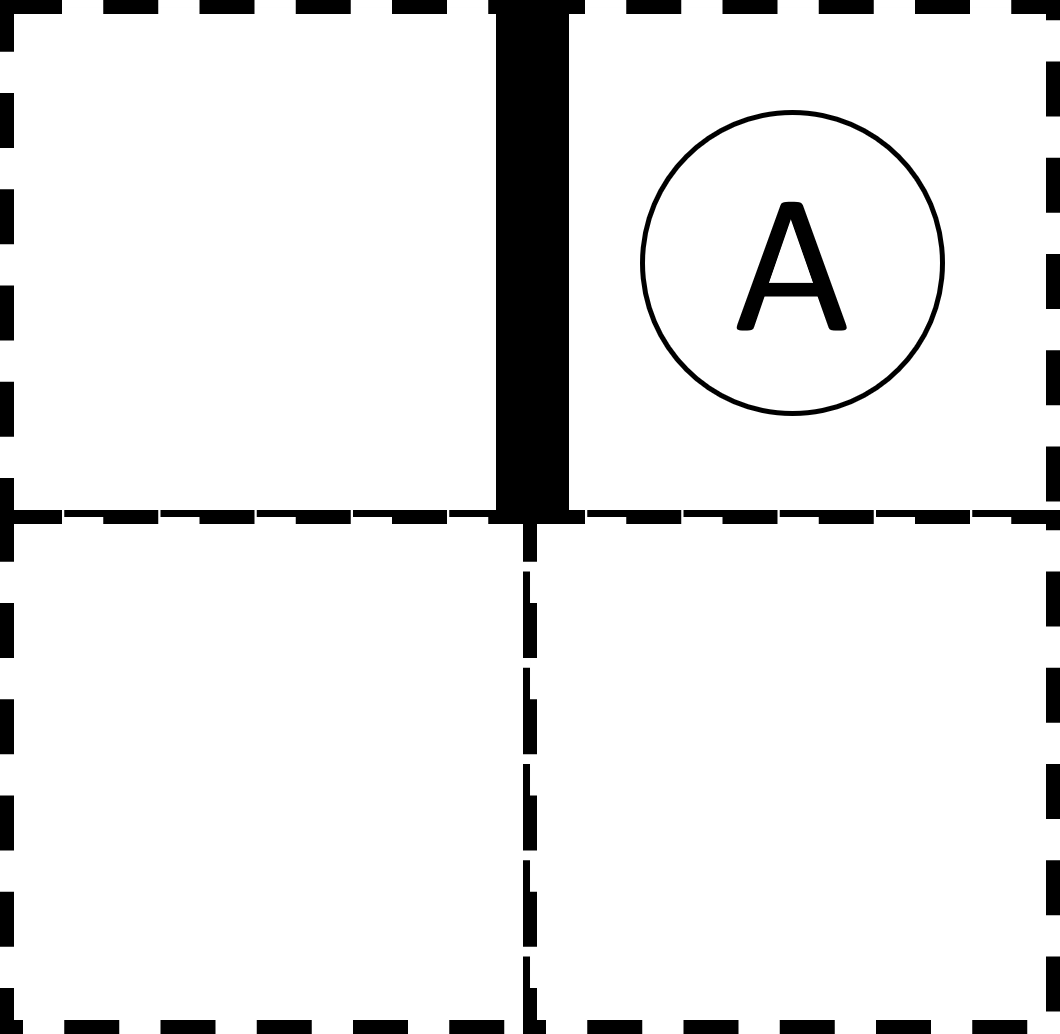
\includegraphics[width=0.5\linewidth]{5BeyondSBDRLGlobalAlgebras/Images/2x2_with_wall_world_states/w1.png}
        \caption{$w_{1}$}
        \vspace{0.25cm}
    \end{subfigure}
    \begin{subfigure}[b]{0.45\linewidth}
        \centering
        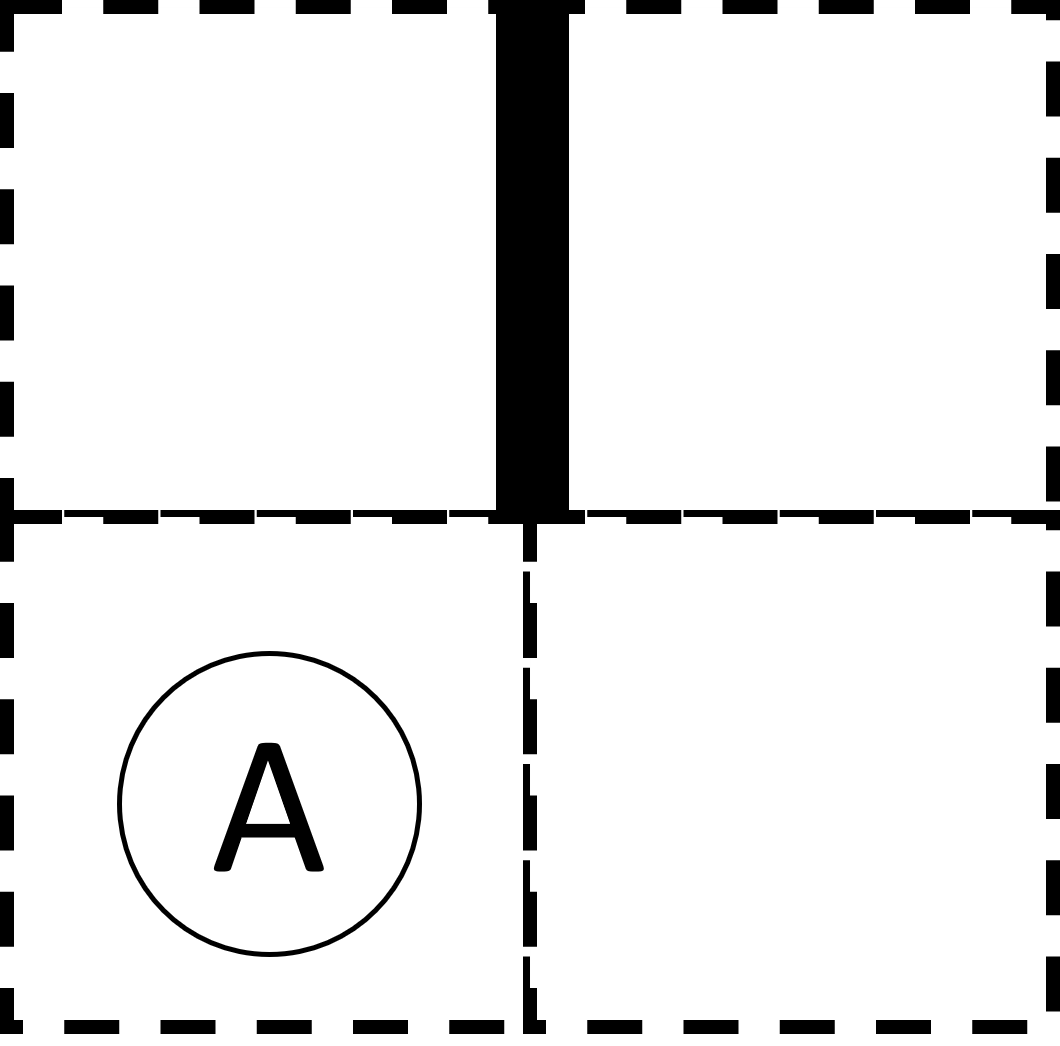
\includegraphics[width=0.5\linewidth]{5BeyondSBDRLGlobalAlgebras/Images/2x2_with_wall_world_states/w2.png}
        \caption{$w_{2}$}
    \end{subfigure}
    \begin{subfigure}[b]{0.45\linewidth}
        \centering
        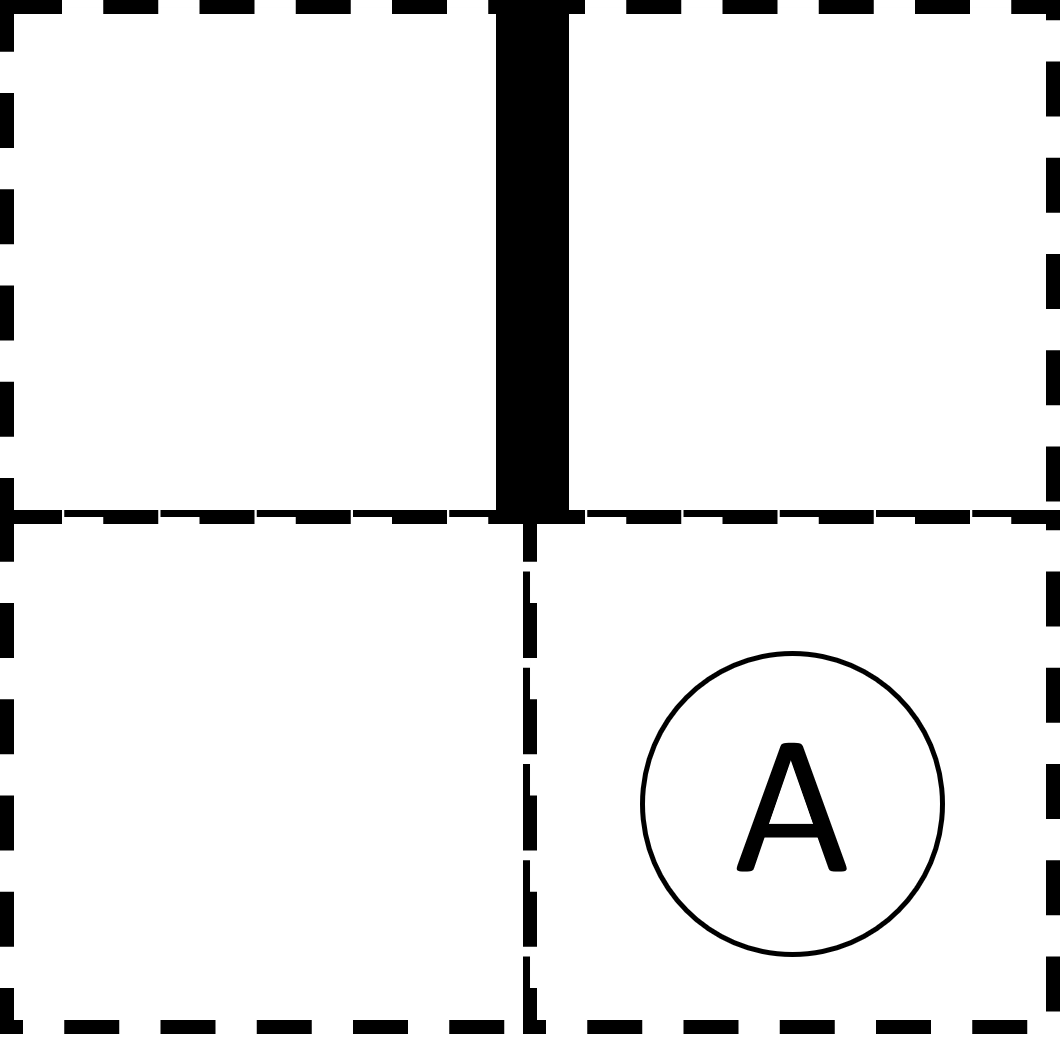
\includegraphics[width=0.5\linewidth]{5BeyondSBDRLGlobalAlgebras/Images/2x2_with_wall_world_states/w3.png}
        \caption{$w_{3}$}
    \end{subfigure}
  \caption{
  The world states of a cyclical $2\times 2$ grid world $\mathscr{W}_{\beta}$ with a wall, where changes to the world are due to an agent moving either north, south, east, or west.
  The position of the agent in the world is represented by the position of the circled A.
  \draftnote{blue}{To do}{Fix figures.}
  }
\label{fig:2x2_cyclical_grid_world_wall_states}
\end{figure}

Our agent has the same minimum actions as in \cref{sec:an_example_world}.
But what happens if $\mathscr{W}_{\beta}$ is in state $w_{0}$ and the agent performs the `move east` action (i.e., the agent tries to move into the wall)?
We say the wall has constrained the actions of the agent, and we consider two treatments of the constrained actions\footnote{
An action $a \in \hat{A}^{*}/\sim$ is called \emph{constrained} in a world state $w \in W$ if we need to choose either a masked treatment or an identity treatment for performing that action in that world state (i.e., we must decide either $a * w = \bot$ or $a * w = w$).
}
\begin{enumerate}
    \item \textbf{Masked treatment.}
    Constrained actions are not allowed to be performed by the agent and so are considered to be \emph{undefined} - they send the world into the undefined state $\bot$; and
    \item \textbf{Identity treatment.}
    Constrained actions can be performed by the agent, but any actions that would have been undefined have the same effect as performing the no-op action $1$.
    \draftnote{blue}{Consider}{
    Does this treatment actually want to treat constrained actions as $\epsilon$?
    What about when we introduce equivalence that depends on time + space ?
    }
\end{enumerate}
These two treatments are commonly used in reinforcement learning \draftnote{blue}{To do}{References.}.

%%%%%%%%%%%%%%%%%%%%%%%%%%%%%%%%%%%%%%%%%%%%%
\subsection{Masked treatment}

\draftnote{blue}{Consider}{
Do we actually not allow an agent to perform the masked action?
}

\Cref{tab:2x2_gridworld_minimum_transformations_wall_masked} shows the minimum action transformations, and \cref{fig:2x2_gridworld_minimum_transformations_wall_masked} is a world diagram containing the $\hat{D}_{A}$ transformations.

\begin{table}[H]
    \centering
    \begin{tabular}{c|c c c c c}
                &  $1$      & $U$       & $D$       & $L$               & $R$\\
         \hline
        $w_{0}$ & $w_{0}$   & $w_{2}$   & $w_{2}$   & $w_{1}$           & \bm{$\bot$} \\
        $w_{1}$ & $w_{1}$   & $w_{3}$   & $w_{3}$   & \bm{$\bot$}         & $w_{0}$ \\
        $w_{2}$ & $w_{2}$   & $w_{0}$   & $w_{0}$   & $w_{3}$           & $w_{3}$ \\
        $w_{3}$ & $w_{3}$   & $w_{1}$   & $w_{1}$   & $w_{2}$           & $w_{2}$ \\
    \end{tabular}
    \caption{
    Each entry in this table shows the result of the outcome state of the agent performing the action given in the column label when in the world state given by the row label (i.e., $(row \; label) * (column \; label)$).
    \draftnote{blue}{To do}{
    Switch the row and column around so it matches Cayley tables (i.e., $(row \; label) \ast (column \; label)$).
    }
    }
    \label{tab:2x2_gridworld_minimum_transformations_wall_masked}
\end{table}

\begin{figure}[H]
    \centering
    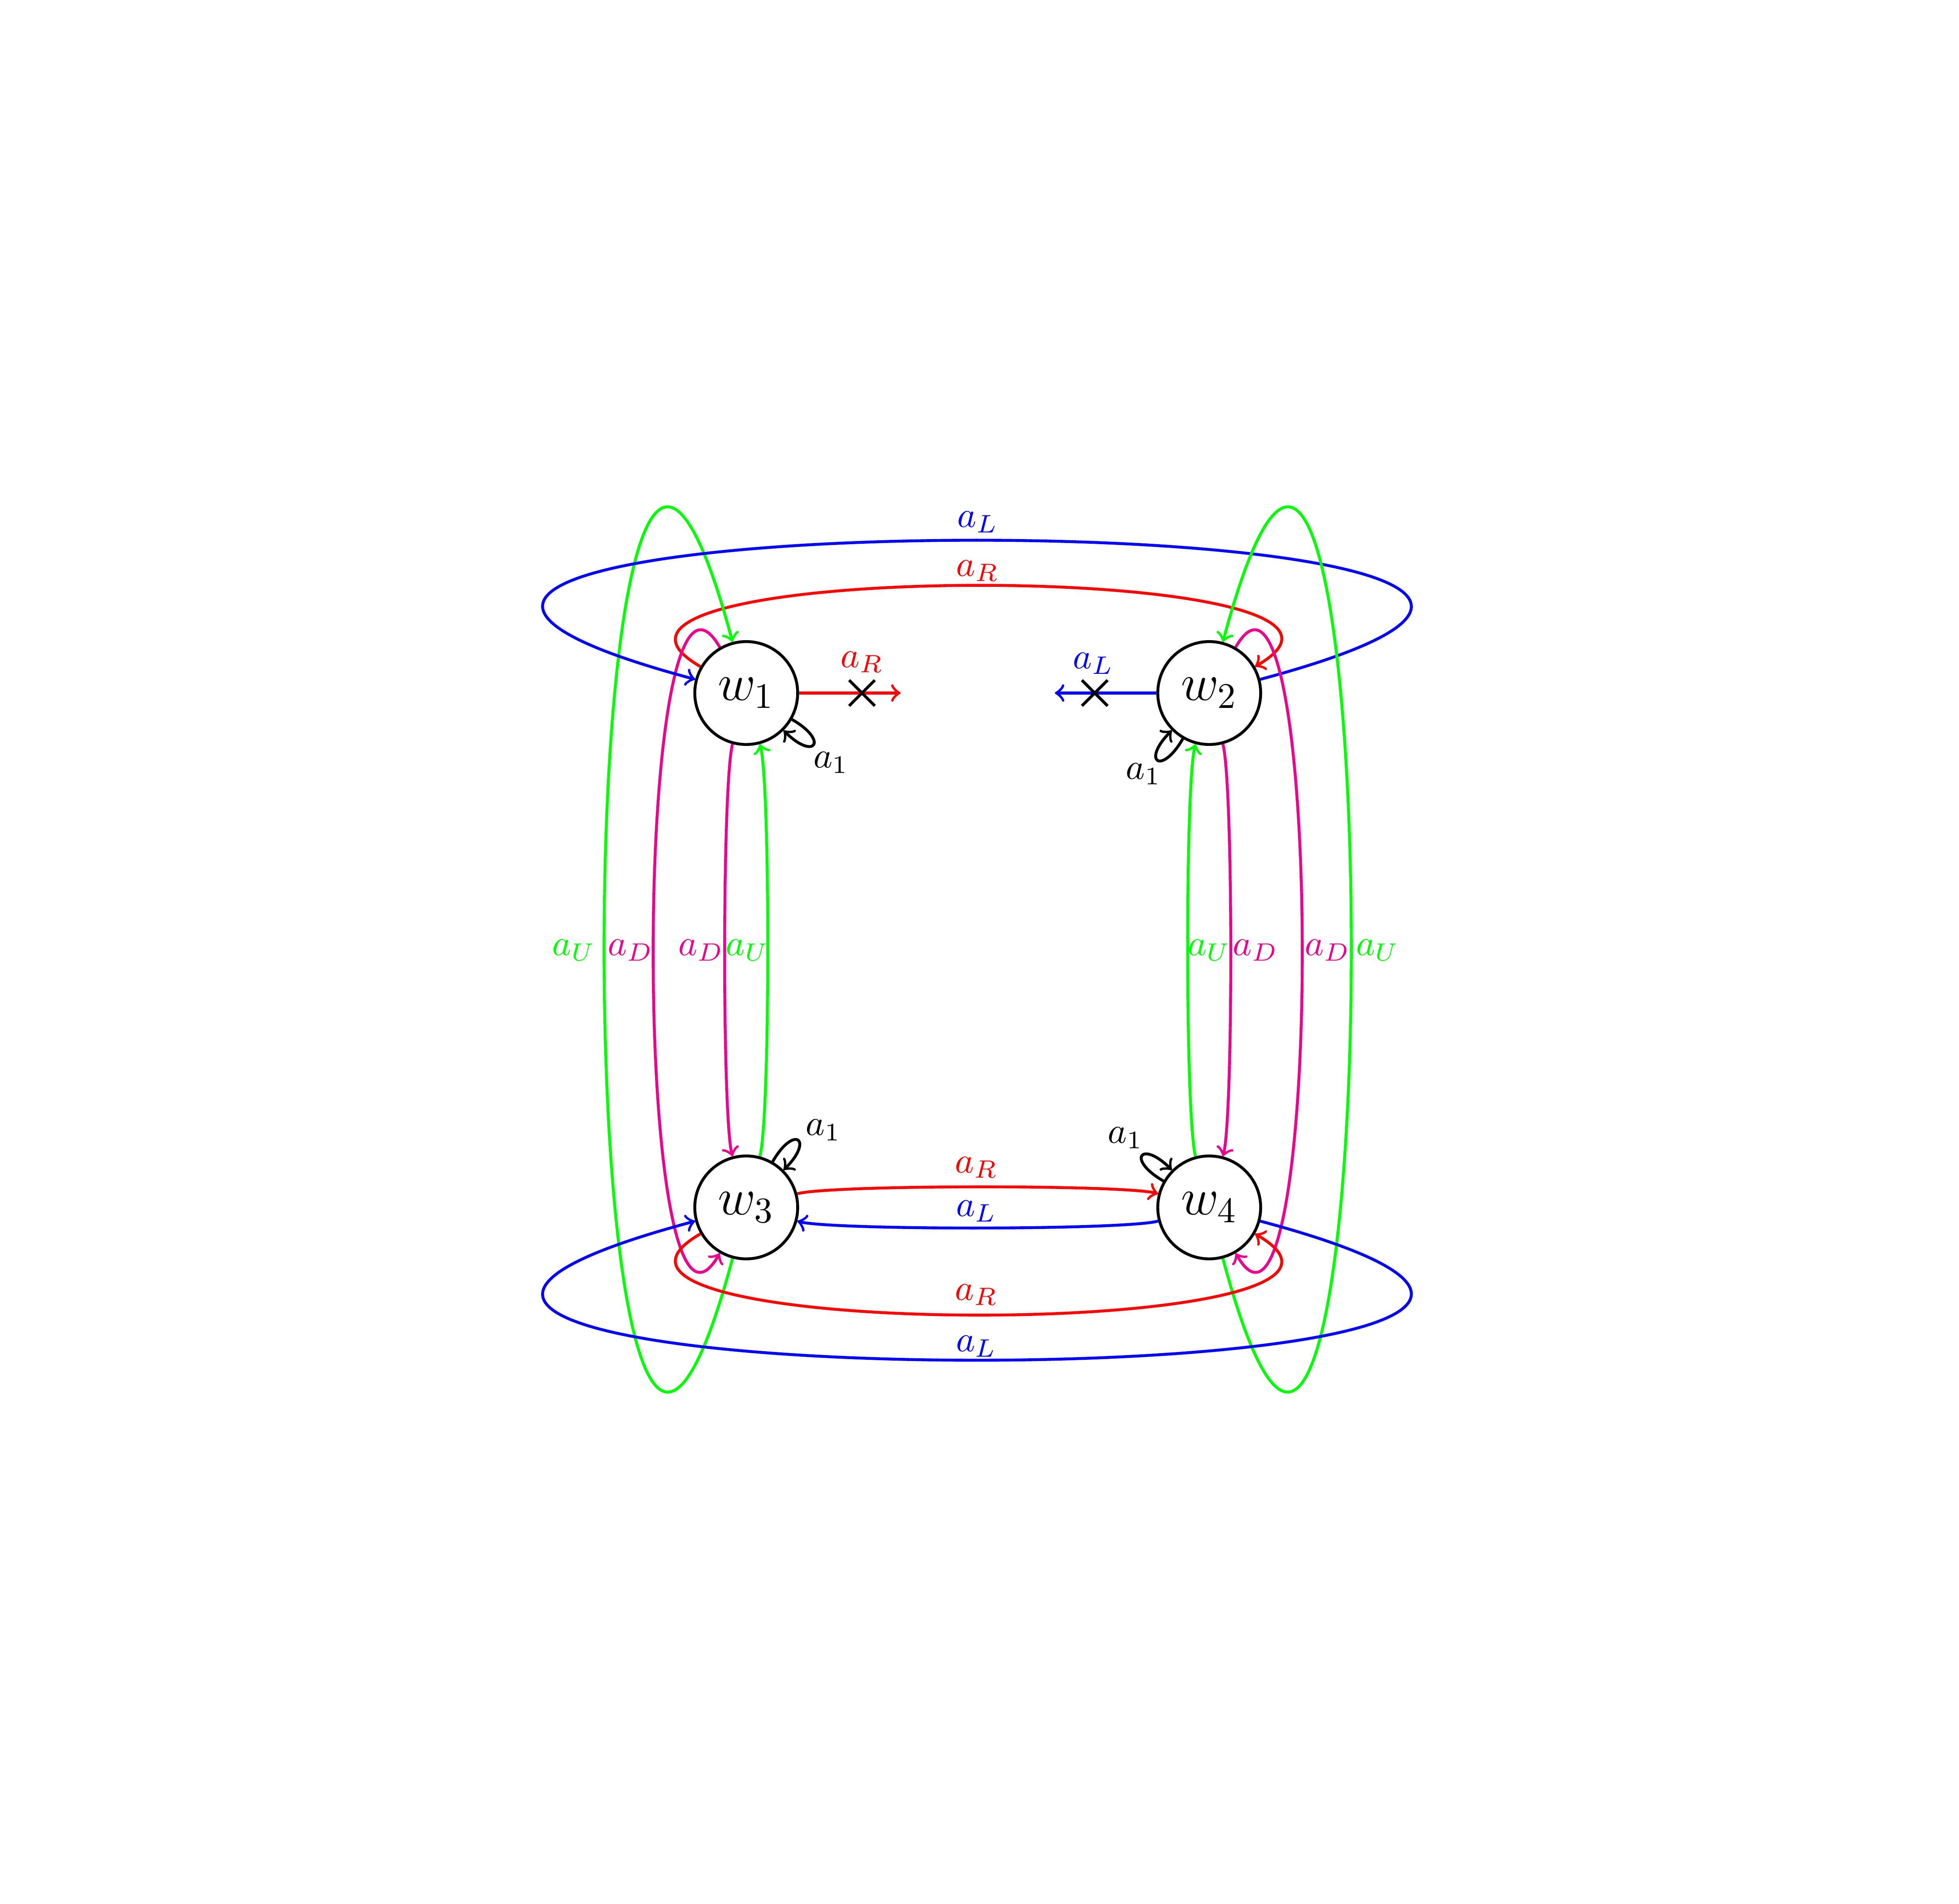
\includegraphics[width=0.75\linewidth]{5BeyondSBDRLGlobalAlgebras/Images/masked_walls_2x2_cyclical_min_actions.drawio.png}
    \caption{
    A world diagram of world $\mathscr{W}_{\beta}$ containing the labelled $\hat{D}_{A}$ transformations for an agent with minimum actions $\hat{A} = \{1, N, S, E, W\}$ using the masked treatment of constrained actions.
    \draftnote{blue}{Consider}{Send arrows explicitly to $\bot$ ?}
    }
    \label{fig:2x2_gridworld_minimum_transformations_wall_masked}
\end{figure}

\begin{table}[H]
\centering
\begin{tabular}{lc}
\hline
\textbf{Property} & \textbf{Present?} \\
\hline
Total & N \\
Associative & Y \\
Identity & Y \\
Inverses & N \\
\hline
Commutative & N \\
\end{tabular}
\caption{
Group properties of $(\hat{A}^{*}/\sim, \circ_{\sim})$ for an agent with $\hat{A} = \{1, E, W, N, S \}$ in world $\mathscr{W}_{\beta}$ with masked treatment.
\draftnote{blue}{To do}{Sort table formatting.}
\draftnote{blue}{Consider}{Include Totality property ?}
}
\end{table}



\begin{fullwidth}
\begin{landscape}
\draftnote{blue}{To do}{
Figure out what to do with this table.
}
\setlength{\tabcolsep}{2pt}
{\fontsize{8}{10}\selectfont
\setlength{\tabcolsep}{4pt}
\begin{longtable}[H]{l|lllllllllllllllllllllllllllllllllllllllllllllllllllllllllll}
 & $1$ & $W$ & $N$ & $S$ & $NW$ & $SW$ & $WN$ & $NN$ & $SN$ & $WS$ & $NS$ & $WNW$ & $NNW$ & $SNW$ & $WSW$ & $NSW$ & $NWN$ & $SWN$ & $WNN$ & $NNN$ & $WSN$ & $NWS$ & $SWS$ & $WNS$ & $NWNW$ & $SWNW$ & $WNNW$ & $NNNW$ & $WSNW$ & $NWSW$ & $SWSW$ & $WNSW$ & $NNWN$ & $SNWN$ & $NSWN$ & $NWNN$ & $SWNN$ & $WNNN$ & $NNWS$ & $SNWS$ & $NSWS$ & $NNWNW$ & $SNWNW$ & $NSWNW$ & $NWNNW$ & $SWNNW$ & $WNNNW$ & $NNWSW$ & $SNWSW$ & $NSWSW$ & $NNNWN$ & $NNWNN$ & $SNWNN$ & $NSWNN$ & $NNNWS$ & $NNNWNW$ & $SNWNNW$ & $NSWNNW$ & $NNNWSW$ \\
\midrule
\endfirsthead
 & $1$ & $W$ & $N$ & $S$ & $NW$ & $SW$ & $WN$ & $NN$ & $SN$ & $WS$ & $NS$ & $WNW$ & $NNW$ & $SNW$ & $WSW$ & $NSW$ & $NWN$ & $SWN$ & $WNN$ & $NNN$ & $WSN$ & $NWS$ & $SWS$ & $WNS$ & $NWNW$ & $SWNW$ & $WNNW$ & $NNNW$ & $WSNW$ & $NWSW$ & $SWSW$ & $WNSW$ & $NNWN$ & $SNWN$ & $NSWN$ & $NWNN$ & $SWNN$ & $WNNN$ & $NNWS$ & $SNWS$ & $NSWS$ & $NNWNW$ & $SNWNW$ & $NSWNW$ & $NWNNW$ & $SWNNW$ & $WNNNW$ & $NNWSW$ & $SNWSW$ & $NSWSW$ & $NNNWN$ & $NNWNN$ & $SNWNN$ & $NSWNN$ & $NNNWS$ & $NNNWNW$ & $SNWNNW$ & $NSWNNW$ & $NNNWSW$ \\
\midrule
\endhead
\midrule
\multicolumn{60}{r}{Continued on next page} \\
\midrule
\endfoot
\endlastfoot
\textbf{$1$} & $1$ & $W$ & $N$ & $S$ & $NW$ & $SW$ & $WN$ & $NN$ & $SN$ & $WS$ & $NS$ & $WNW$ & $NNW$ & $SNW$ & $WSW$ & $NSW$ & $NWN$ & $SWN$ & $WNN$ & $NNN$ & $WSN$ & $NWS$ & $SWS$ & $WNS$ & $NWNW$ & $SWNW$ & $WNNW$ & $NNNW$ & $WSNW$ & $NWSW$ & $SWSW$ & $WNSW$ & $NNWN$ & $SNWN$ & $NSWN$ & $NWNN$ & $SWNN$ & $WNNN$ & $NNWS$ & $SNWS$ & $NSWS$ & $NNWNW$ & $SNWNW$ & $NSWNW$ & $NWNNW$ & $SWNNW$ & $WNNNW$ & $NNWSW$ & $SNWSW$ & $NSWSW$ & $NNNWN$ & $NNWNN$ & $SNWNN$ & $NSWNN$ & $NNNWS$ & $NNNWNW$ & $SNWNNW$ & $NSWNNW$ & $NNNWSW$ \\
\textbf{$W$} & $W$ & $1$ & $WN$ & $WS$ & $WNW$ & $WSW$ & $N$ & $WNN$ & $WSN$ & $S$ & $WNS$ & $NW$ & $WNNW$ & $WSNW$ & $SW$ & $WNSW$ & $SWSW$ & $SWNW$ & $NN$ & $WNNN$ & $SN$ & $NWSW$ & $NWNW$ & $NS$ & $SWS$ & $SWN$ & $NNW$ & $WNNNW$ & $SNW$ & $NWS$ & $NWN$ & $NSW$ & $NWNNW$ & $NSWSW$ & $NSWNW$ & $NNWNW$ & $NNWSW$ & $NNN$ & $SWNNW$ & $SNWSW$ & $SNWNW$ & $NWNN$ & $NSWS$ & $NSWN$ & $NNWN$ & $NNWS$ & $NNNW$ & $SWNN$ & $SNWS$ & $SNWN$ & $SNWNNW$ & $NNWNN$ & $NNNWNW$ & $NNNWSW$ & $NSWNNW$ & $SNWNN$ & $NNNWN$ & $NNNWS$ & $NSWNN$ \\
\textbf{$N$} & $N$ & $NW$ & $NN$ & $NS$ & $NNW$ & $NSW$ & $NWN$ & $NNN$ & $N$ & $NWS$ & $NNN$ & $NWNW$ & $NNNW$ & $NW$ & $NWSW$ & $NNNW$ & $NNWN$ & $NSWN$ & $NWNN$ & $NN$ & $NSWN$ & $NNWS$ & $NSWS$ & $NSWS$ & $NNWNW$ & $NSWNW$ & $NWNNW$ & $NNW$ & $NSWNW$ & $NNWSW$ & $NSWSW$ & $NSWSW$ & $NNNWN$ & $NWN$ & $NNNWN$ & $NNWNN$ & $NSWNN$ & $NSWNN$ & $NNNWS$ & $NWS$ & $NNNWS$ & $NNNWNW$ & $NWNW$ & $NNNWNW$ & $NNWNN$ & $NSWNNW$ & $NSWNNW$ & $NNNWSW$ & $NWSW$ & $NNNWSW$ & $NNWN$ & $NNWNN$ & $NWNN$ & $NNWNN$ & $NNWS$ & $NNWNW$ & $NWNNW$ & $NNWNN$ & $NNWSW$ \\
\textbf{$S$} & $S$ & $SW$ & $SN$ & $NN$ & $SNW$ & $NNW$ & $SWN$ & $NNN$ & $NNN$ & $SWS$ & $S$ & $SWNW$ & $NNNW$ & $NNNW$ & $SWSW$ & $SW$ & $SNWN$ & $NNWN$ & $SWNN$ & $NN$ & $SNWN$ & $SNWS$ & $NNWS$ & $SNWS$ & $SNWNW$ & $NNWNW$ & $SWNNW$ & $NNW$ & $SNWNW$ & $SNWSW$ & $NNWSW$ & $SNWSW$ & $NNNWN$ & $NNNWN$ & $SWN$ & $SNWNN$ & $NNWNN$ & $SNWNN$ & $NNNWS$ & $NNNWS$ & $SWS$ & $NNNWNW$ & $NNNWNW$ & $SWNW$ & $SNWNNW$ & $NNWNN$ & $SNWNNW$ & $NNNWSW$ & $NNNWSW$ & $SWSW$ & $NNWN$ & $NNWNN$ & $NNWNN$ & $SWNN$ & $NNWS$ & $NNWNW$ & $NNWNN$ & $SWNNW$ & $NNWSW$ \\
\textbf{$NW$} & $NW$ & $N$ & $NWN$ & $NWS$ & $NWNW$ & $NWSW$ & $NN$ & $NWNN$ & $NSWN$ & $NS$ & $NSWS$ & $NNW$ & $NWNNW$ & $NSWNW$ & $NSW$ & $NSWSW$ & $NSWSW$ & $NSWNW$ & $NNN$ & $NSWNN$ & $N$ & $NNWSW$ & $NNWNW$ & $NNN$ & $NSWS$ & $NSWN$ & $NNNW$ & $NSWNNW$ & $NW$ & $NNWS$ & $NNWN$ & $NNNW$ & $NNWNN$ & $NNNWSW$ & $NNNWNW$ & $NNNWNW$ & $NNNWSW$ & $NN$ & $NSWNNW$ & $NWSW$ & $NWNW$ & $NNWNN$ & $NNNWS$ & $NNNWN$ & $NNNWN$ & $NNNWS$ & $NNW$ & $NSWNN$ & $NWS$ & $NWN$ & $NWNNW$ & $NNWNN$ & $NNWNW$ & $NNWSW$ & $NNWNN$ & $NWNN$ & $NNWN$ & $NNWS$ & $NNWNN$ \\
\textbf{$SW$} & $SW$ & $S$ & $SWN$ & $SWS$ & $SWNW$ & $SWSW$ & $SN$ & $SWNN$ & $SNWN$ & $NN$ & $SNWS$ & $SNW$ & $SWNNW$ & $SNWNW$ & $NNW$ & $SNWSW$ & $NNWSW$ & $NNWNW$ & $NNN$ & $SNWNN$ & $NNN$ & $SNWSW$ & $SNWNW$ & $S$ & $NNWS$ & $NNWN$ & $NNNW$ & $SNWNNW$ & $NNNW$ & $SNWS$ & $SNWN$ & $SW$ & $SNWNNW$ & $SWSW$ & $SWNW$ & $NNNWNW$ & $NNNWSW$ & $NN$ & $NNWNN$ & $NNNWSW$ & $NNNWNW$ & $SNWNN$ & $SWS$ & $SWN$ & $NNNWN$ & $NNNWS$ & $NNW$ & $NNWNN$ & $NNNWS$ & $NNNWN$ & $NNWNN$ & $NNWNN$ & $NNWNW$ & $NNWSW$ & $SWNNW$ & $NNWNN$ & $NNWN$ & $NNWS$ & $SWNN$ \\
\textbf{$WN$} & $WN$ & $WNW$ & $WNN$ & $WNS$ & $WNNW$ & $WNSW$ & $SWSW$ & $WNNN$ & $WN$ & $NWSW$ & $WNNN$ & $SWS$ & $WNNNW$ & $WNW$ & $NWS$ & $WNNNW$ & $NWNNW$ & $NSWNW$ & $NNWNW$ & $WNN$ & $NSWNW$ & $SWNNW$ & $SNWNW$ & $SNWNW$ & $NWNN$ & $NSWN$ & $NNWN$ & $WNNW$ & $NSWN$ & $SWNN$ & $SNWN$ & $SNWN$ & $SNWNNW$ & $SWSW$ & $SNWNNW$ & $NNWNN$ & $NNNWSW$ & $NNNWSW$ & $NSWNNW$ & $NWSW$ & $NSWNNW$ & $SNWNN$ & $SWS$ & $SNWNN$ & $NNWNN$ & $NNNWS$ & $NNNWS$ & $NSWNN$ & $NWS$ & $NSWNN$ & $NWNNW$ & $NNWNN$ & $NNWNW$ & $NNWNN$ & $SWNNW$ & $NWNN$ & $NNWN$ & $NNWNN$ & $SWNN$ \\
\textbf{$NN$} & $NN$ & $NNW$ & $NNN$ & $NNN$ & $NNNW$ & $NNNW$ & $NNWN$ & $NN$ & $NN$ & $NNWS$ & $NN$ & $NNWNW$ & $NNW$ & $NNW$ & $NNWSW$ & $NNW$ & $NNNWN$ & $NNNWN$ & $NNWNN$ & $NNN$ & $NNNWN$ & $NNNWS$ & $NNNWS$ & $NNNWS$ & $NNNWNW$ & $NNNWNW$ & $NNWNN$ & $NNNW$ & $NNNWNW$ & $NNNWSW$ & $NNNWSW$ & $NNNWSW$ & $NNWN$ & $NNWN$ & $NNWN$ & $NNWNN$ & $NNWNN$ & $NNWNN$ & $NNWS$ & $NNWS$ & $NNWS$ & $NNWNW$ & $NNWNW$ & $NNWNW$ & $NNWNN$ & $NNWNN$ & $NNWNN$ & $NNWSW$ & $NNWSW$ & $NNWSW$ & $NNNWN$ & $NNWNN$ & $NNWNN$ & $NNWNN$ & $NNNWS$ & $NNNWNW$ & $NNWNN$ & $NNWNN$ & $NNNWSW$ \\
\textbf{$SN$} & $SN$ & $SNW$ & $NNN$ & $S$ & $NNNW$ & $SW$ & $SNWN$ & $NN$ & $SN$ & $SNWS$ & $NN$ & $SNWNW$ & $NNW$ & $SNW$ & $SNWSW$ & $NNW$ & $NNNWN$ & $SWN$ & $SNWNN$ & $NNN$ & $SWN$ & $NNNWS$ & $SWS$ & $SWS$ & $NNNWNW$ & $SWNW$ & $SNWNNW$ & $NNNW$ & $SWNW$ & $NNNWSW$ & $SWSW$ & $SWSW$ & $NNWN$ & $SNWN$ & $NNWN$ & $NNWNN$ & $SWNN$ & $SWNN$ & $NNWS$ & $SNWS$ & $NNWS$ & $NNWNW$ & $SNWNW$ & $NNWNW$ & $NNWNN$ & $SWNNW$ & $SWNNW$ & $NNWSW$ & $SNWSW$ & $NNWSW$ & $NNNWN$ & $NNWNN$ & $SNWNN$ & $NNWNN$ & $NNNWS$ & $NNNWNW$ & $SNWNNW$ & $NNWNN$ & $NNNWSW$ \\
\textbf{$WS$} & $WS$ & $WSW$ & $WSN$ & $WNN$ & $WSNW$ & $WNNW$ & $SWNW$ & $WNNN$ & $WNNN$ & $NWNW$ & $WS$ & $SWN$ & $WNNNW$ & $WNNNW$ & $NWN$ & $WSW$ & $NSWSW$ & $NWNNW$ & $NNWSW$ & $WNN$ & $NSWSW$ & $SNWSW$ & $SWNNW$ & $SNWSW$ & $NSWS$ & $NWNN$ & $NNWS$ & $WNNW$ & $NSWS$ & $SNWS$ & $SWNN$ & $SNWS$ & $SNWNNW$ & $SNWNNW$ & $SWNW$ & $NNNWNW$ & $NNWNN$ & $NNNWNW$ & $NSWNNW$ & $NSWNNW$ & $NWNW$ & $SNWNN$ & $SNWNN$ & $SWN$ & $NNNWN$ & $NNWNN$ & $NNNWN$ & $NSWNN$ & $NSWNN$ & $NWN$ & $NWNNW$ & $NNWNN$ & $NNWNN$ & $NNWSW$ & $SWNNW$ & $NWNN$ & $NNWNN$ & $NNWS$ & $SWNN$ \\
\textbf{$NS$} & $NS$ & $NSW$ & $N$ & $NNN$ & $NW$ & $NNNW$ & $NSWN$ & $NN$ & $NN$ & $NSWS$ & $NS$ & $NSWNW$ & $NNW$ & $NNW$ & $NSWSW$ & $NSW$ & $NWN$ & $NNNWN$ & $NSWNN$ & $NNN$ & $NWN$ & $NWS$ & $NNNWS$ & $NWS$ & $NWNW$ & $NNNWNW$ & $NSWNNW$ & $NNNW$ & $NWNW$ & $NWSW$ & $NNNWSW$ & $NWSW$ & $NNWN$ & $NNWN$ & $NSWN$ & $NWNN$ & $NNWNN$ & $NWNN$ & $NNWS$ & $NNWS$ & $NSWS$ & $NNWNW$ & $NNWNW$ & $NSWNW$ & $NWNNW$ & $NNWNN$ & $NWNNW$ & $NNWSW$ & $NNWSW$ & $NSWSW$ & $NNNWN$ & $NNWNN$ & $NNWNN$ & $NSWNN$ & $NNNWS$ & $NNNWNW$ & $NNWNN$ & $NSWNNW$ & $NNNWSW$ \\
\textbf{$WNW$} & $WNW$ & $WN$ & $SWSW$ & $NWSW$ & $SWS$ & $NWS$ & $WNN$ & $NNWNW$ & $NSWNW$ & $WNS$ & $SNWNW$ & $WNNW$ & $NNWN$ & $NSWN$ & $WNSW$ & $SNWN$ & $SNWN$ & $NSWN$ & $WNNN$ & $NNNWSW$ & $WN$ & $SWNN$ & $NWNN$ & $WNNN$ & $SNWNW$ & $NSWNW$ & $WNNNW$ & $NNNWS$ & $WNW$ & $SWNNW$ & $NWNNW$ & $WNNNW$ & $NNWNN$ & $NSWNN$ & $SNWNN$ & $SNWNN$ & $NSWNN$ & $WNN$ & $NNNWS$ & $NWS$ & $SWS$ & $NNWNN$ & $NSWNNW$ & $SNWNNW$ & $SNWNNW$ & $NSWNNW$ & $WNNW$ & $NNNWSW$ & $NWSW$ & $SWSW$ & $NNWN$ & $NNWNN$ & $NWNN$ & $SWNN$ & $NNWNN$ & $NNWNW$ & $NWNNW$ & $SWNNW$ & $NNWNN$ \\
\textbf{$NNW$} & $NNW$ & $NN$ & $NNWN$ & $NNWS$ & $NNWNW$ & $NNWSW$ & $NNN$ & $NNWNN$ & $NNNWN$ & $NNN$ & $NNNWS$ & $NNNW$ & $NNWNN$ & $NNNWNW$ & $NNNW$ & $NNNWSW$ & $NNNWSW$ & $NNNWNW$ & $NN$ & $NNWNN$ & $NN$ & $NNNWSW$ & $NNNWNW$ & $NN$ & $NNNWS$ & $NNNWN$ & $NNW$ & $NNWNN$ & $NNW$ & $NNNWS$ & $NNNWN$ & $NNW$ & $NNWNN$ & $NNWSW$ & $NNWNW$ & $NNWNW$ & $NNWSW$ & $NNN$ & $NNWNN$ & $NNWSW$ & $NNWNW$ & $NNWNN$ & $NNWS$ & $NNWN$ & $NNWN$ & $NNWS$ & $NNNW$ & $NNWNN$ & $NNWS$ & $NNWN$ & $NNWNN$ & $NNWNN$ & $NNNWNW$ & $NNNWSW$ & $NNWNN$ & $NNWNN$ & $NNNWN$ & $NNNWS$ & $NNWNN$ \\
\textbf{$SNW$} & $SNW$ & $SN$ & $SNWN$ & $SNWS$ & $SNWNW$ & $SNWSW$ & $NNN$ & $SNWNN$ & $SWN$ & $S$ & $SWS$ & $NNNW$ & $SNWNNW$ & $SWNW$ & $SW$ & $SWSW$ & $SWSW$ & $SWNW$ & $NN$ & $SWNN$ & $SN$ & $NNNWSW$ & $NNNWNW$ & $NN$ & $SWS$ & $SWN$ & $NNW$ & $SWNNW$ & $SNW$ & $NNNWS$ & $NNNWN$ & $NNW$ & $NNWNN$ & $NNWSW$ & $NNWNW$ & $NNWNW$ & $NNWSW$ & $NNN$ & $SWNNW$ & $SNWSW$ & $SNWNW$ & $NNWNN$ & $NNWS$ & $NNWN$ & $NNWN$ & $NNWS$ & $NNNW$ & $SWNN$ & $SNWS$ & $SNWN$ & $SNWNNW$ & $NNWNN$ & $NNNWNW$ & $NNNWSW$ & $NNWNN$ & $SNWNN$ & $NNNWN$ & $NNNWS$ & $NNWNN$ \\
\textbf{$WSW$} & $WSW$ & $WS$ & $SWNW$ & $NWNW$ & $SWN$ & $NWN$ & $WSN$ & $NNWSW$ & $NSWSW$ & $WNN$ & $SNWSW$ & $WSNW$ & $NNWS$ & $NSWS$ & $WNNW$ & $SNWS$ & $SWNN$ & $NWNN$ & $WNNN$ & $NNNWNW$ & $WNNN$ & $SNWS$ & $NSWS$ & $WS$ & $SWNNW$ & $NWNNW$ & $WNNNW$ & $NNNWN$ & $WNNNW$ & $SNWSW$ & $NSWSW$ & $WSW$ & $NNNWN$ & $NWN$ & $SWN$ & $SNWNN$ & $NSWNN$ & $WNN$ & $NNWNN$ & $NSWNN$ & $SNWNN$ & $NNNWNW$ & $NWNW$ & $SWNW$ & $SNWNNW$ & $NSWNNW$ & $WNNW$ & $NNWNN$ & $NSWNNW$ & $SNWNNW$ & $NNWNN$ & $NNWNN$ & $NWNN$ & $SWNN$ & $NNWS$ & $NNWNN$ & $NWNNW$ & $SWNNW$ & $NNWSW$ \\
\textbf{$NSW$} & $NSW$ & $NS$ & $NSWN$ & $NSWS$ & $NSWNW$ & $NSWSW$ & $N$ & $NSWNN$ & $NWN$ & $NNN$ & $NWS$ & $NW$ & $NSWNNW$ & $NWNW$ & $NNNW$ & $NWSW$ & $NNNWSW$ & $NNNWNW$ & $NN$ & $NWNN$ & $NN$ & $NWSW$ & $NWNW$ & $NS$ & $NNNWS$ & $NNNWN$ & $NNW$ & $NWNNW$ & $NNW$ & $NWS$ & $NWN$ & $NSW$ & $NWNNW$ & $NSWSW$ & $NSWNW$ & $NNWNW$ & $NNWSW$ & $NNN$ & $NNWNN$ & $NNWSW$ & $NNWNW$ & $NWNN$ & $NSWS$ & $NSWN$ & $NNWN$ & $NNWS$ & $NNNW$ & $NNWNN$ & $NNWS$ & $NNWN$ & $NNWNN$ & $NNWNN$ & $NNNWNW$ & $NNNWSW$ & $NSWNNW$ & $NNWNN$ & $NNNWN$ & $NNNWS$ & $NSWNN$ \\
\textbf{$NWN$} & $NWN$ & $NWNW$ & $NWNN$ & $NSWS$ & $NWNNW$ & $NSWSW$ & $NSWSW$ & $NSWNN$ & $NWN$ & $NNWSW$ & $NSWNN$ & $NSWS$ & $NSWNNW$ & $NWNW$ & $NNWS$ & $NSWNNW$ & $NNWNN$ & $NNNWNW$ & $NNNWNW$ & $NWNN$ & $NNNWNW$ & $NSWNNW$ & $NWNW$ & $NWNW$ & $NNWNN$ & $NNNWN$ & $NNNWN$ & $NWNNW$ & $NNNWN$ & $NSWNN$ & $NWN$ & $NWN$ & $NWNNW$ & $NSWSW$ & $NWNNW$ & $NNWNN$ & $NNWSW$ & $NNWSW$ & $NNWNN$ & $NNWSW$ & $NNWNN$ & $NWNN$ & $NSWS$ & $NWNN$ & $NNWNN$ & $NNWS$ & $NNWS$ & $NNWNN$ & $NNWS$ & $NNWNN$ & $NNWNN$ & $NNWNN$ & $NNNWNW$ & $NNWNN$ & $NSWNNW$ & $NNWNN$ & $NNNWN$ & $NNWNN$ & $NSWNN$ \\
\textbf{$SWN$} & $SWN$ & $SWNW$ & $SWNN$ & $SNWS$ & $SWNNW$ & $SNWSW$ & $NNWSW$ & $SNWNN$ & $SWN$ & $SNWSW$ & $SNWNN$ & $NNWS$ & $SNWNNW$ & $SWNW$ & $SNWS$ & $SNWNNW$ & $SNWNNW$ & $SWNW$ & $NNNWNW$ & $SWNN$ & $SWNW$ & $NNWNN$ & $NNNWNW$ & $NNNWNW$ & $SNWNN$ & $SWN$ & $NNNWN$ & $SWNNW$ & $SWN$ & $NNWNN$ & $NNNWN$ & $NNNWN$ & $NNWNN$ & $NNWSW$ & $NNWNN$ & $NNWNN$ & $NNWSW$ & $NNWSW$ & $SWNNW$ & $SNWSW$ & $SWNNW$ & $NNWNN$ & $NNWS$ & $NNWNN$ & $NNWNN$ & $NNWS$ & $NNWS$ & $SWNN$ & $SNWS$ & $SWNN$ & $SNWNNW$ & $NNWNN$ & $NNNWNW$ & $NNWNN$ & $NNWNN$ & $SNWNN$ & $NNNWN$ & $NNWNN$ & $NNWNN$ \\
\textbf{$WNN$} & $WNN$ & $WNNW$ & $WNNN$ & $WNNN$ & $WNNNW$ & $WNNNW$ & $NWNNW$ & $WNN$ & $WNN$ & $SWNNW$ & $WNN$ & $NWNN$ & $WNNW$ & $WNNW$ & $SWNN$ & $WNNW$ & $SNWNNW$ & $SNWNNW$ & $NNWNN$ & $WNNN$ & $SNWNNW$ & $NSWNNW$ & $NSWNNW$ & $NSWNNW$ & $SNWNN$ & $SNWNN$ & $NNWNN$ & $WNNNW$ & $SNWNN$ & $NSWNN$ & $NSWNN$ & $NSWNN$ & $NWNNW$ & $NWNNW$ & $NWNNW$ & $NNWNN$ & $NNWNN$ & $NNWNN$ & $SWNNW$ & $SWNNW$ & $SWNNW$ & $NWNN$ & $NWNN$ & $NWNN$ & $NNWNN$ & $NNWNN$ & $NNWNN$ & $SWNN$ & $SWNN$ & $SWNN$ & $SNWNNW$ & $NNWNN$ & $NNWNN$ & $NNWNN$ & $NSWNNW$ & $SNWNN$ & $NNWNN$ & $NNWNN$ & $NSWNN$ \\
\textbf{$NNN$} & $NNN$ & $NNNW$ & $NN$ & $NN$ & $NNW$ & $NNW$ & $NNNWN$ & $NNN$ & $NNN$ & $NNNWS$ & $NNN$ & $NNNWNW$ & $NNNW$ & $NNNW$ & $NNNWSW$ & $NNNW$ & $NNWN$ & $NNWN$ & $NNWNN$ & $NN$ & $NNWN$ & $NNWS$ & $NNWS$ & $NNWS$ & $NNWNW$ & $NNWNW$ & $NNWNN$ & $NNW$ & $NNWNW$ & $NNWSW$ & $NNWSW$ & $NNWSW$ & $NNNWN$ & $NNNWN$ & $NNNWN$ & $NNWNN$ & $NNWNN$ & $NNWNN$ & $NNNWS$ & $NNNWS$ & $NNNWS$ & $NNNWNW$ & $NNNWNW$ & $NNNWNW$ & $NNWNN$ & $NNWNN$ & $NNWNN$ & $NNNWSW$ & $NNNWSW$ & $NNNWSW$ & $NNWN$ & $NNWNN$ & $NNWNN$ & $NNWNN$ & $NNWS$ & $NNWNW$ & $NNWNN$ & $NNWNN$ & $NNWSW$ \\
\textbf{$WSN$} & $WSN$ & $WSNW$ & $WNNN$ & $WS$ & $WNNNW$ & $WSW$ & $NSWSW$ & $WNN$ & $WSN$ & $SNWSW$ & $WNN$ & $NSWS$ & $WNNW$ & $WSNW$ & $SNWS$ & $WNNW$ & $SNWNNW$ & $SWNW$ & $NNNWNW$ & $WNNN$ & $SWNW$ & $NSWNNW$ & $NWNW$ & $NWNW$ & $SNWNN$ & $SWN$ & $NNNWN$ & $WNNNW$ & $SWN$ & $NSWNN$ & $NWN$ & $NWN$ & $NWNNW$ & $NSWSW$ & $NWNNW$ & $NNWNN$ & $NNWSW$ & $NNWSW$ & $SWNNW$ & $SNWSW$ & $SWNNW$ & $NWNN$ & $NSWS$ & $NWNN$ & $NNWNN$ & $NNWS$ & $NNWS$ & $SWNN$ & $SNWS$ & $SWNN$ & $SNWNNW$ & $NNWNN$ & $NNNWNW$ & $NNWNN$ & $NSWNNW$ & $SNWNN$ & $NNNWN$ & $NNWNN$ & $NSWNN$ \\
\textbf{$NWS$} & $NWS$ & $NWSW$ & $NSWN$ & $NWNN$ & $NSWNW$ & $NWNNW$ & $NSWNW$ & $NSWNN$ & $NSWNN$ & $NNWNW$ & $NWS$ & $NSWN$ & $NSWNNW$ & $NSWNNW$ & $NNWN$ & $NWSW$ & $NNNWSW$ & $NNWNN$ & $NNNWSW$ & $NWNN$ & $NNNWSW$ & $NWSW$ & $NSWNNW$ & $NWSW$ & $NNNWS$ & $NNWNN$ & $NNNWS$ & $NWNNW$ & $NNNWS$ & $NWS$ & $NSWNN$ & $NWS$ & $NWNNW$ & $NWNNW$ & $NSWNW$ & $NNWNW$ & $NNWNN$ & $NNWNW$ & $NNWNN$ & $NNWNN$ & $NNWNW$ & $NWNN$ & $NWNN$ & $NSWN$ & $NNWN$ & $NNWNN$ & $NNWN$ & $NNWNN$ & $NNWNN$ & $NNWN$ & $NNWNN$ & $NNWNN$ & $NNWNN$ & $NNNWSW$ & $NSWNNW$ & $NNWNN$ & $NNWNN$ & $NNNWS$ & $NSWNN$ \\
\textbf{$SWS$} & $SWS$ & $SWSW$ & $SNWN$ & $SWNN$ & $SNWNW$ & $SWNNW$ & $NNWNW$ & $SNWNN$ & $SNWNN$ & $SNWNW$ & $SWS$ & $NNWN$ & $SNWNNW$ & $SNWNNW$ & $SNWN$ & $SWSW$ & $SWSW$ & $SNWNNW$ & $NNNWSW$ & $SWNN$ & $SWSW$ & $NNNWSW$ & $NNWNN$ & $NNNWSW$ & $SWS$ & $SNWNN$ & $NNNWS$ & $SWNNW$ & $SWS$ & $NNNWS$ & $NNWNN$ & $NNNWS$ & $NNWNN$ & $NNWNN$ & $NNWNW$ & $NNWNW$ & $NNWNN$ & $NNWNW$ & $SWNNW$ & $SWNNW$ & $SNWNW$ & $NNWNN$ & $NNWNN$ & $NNWN$ & $NNWN$ & $NNWNN$ & $NNWN$ & $SWNN$ & $SWNN$ & $SNWN$ & $SNWNNW$ & $NNWNN$ & $NNWNN$ & $NNNWSW$ & $NNWNN$ & $SNWNN$ & $NNWNN$ & $NNNWS$ & $NNWNN$ \\
\textbf{$WNS$} & $WNS$ & $WNSW$ & $WN$ & $WNNN$ & $WNW$ & $WNNNW$ & $NSWNW$ & $WNN$ & $WNN$ & $SNWNW$ & $WNS$ & $NSWN$ & $WNNW$ & $WNNW$ & $SNWN$ & $WNSW$ & $SWSW$ & $SNWNNW$ & $NNNWSW$ & $WNNN$ & $SWSW$ & $NWSW$ & $NSWNNW$ & $NWSW$ & $SWS$ & $SNWNN$ & $NNNWS$ & $WNNNW$ & $SWS$ & $NWS$ & $NSWNN$ & $NWS$ & $NWNNW$ & $NWNNW$ & $NSWNW$ & $NNWNW$ & $NNWNN$ & $NNWNW$ & $SWNNW$ & $SWNNW$ & $SNWNW$ & $NWNN$ & $NWNN$ & $NSWN$ & $NNWN$ & $NNWNN$ & $NNWN$ & $SWNN$ & $SWNN$ & $SNWN$ & $SNWNNW$ & $NNWNN$ & $NNWNN$ & $NNNWSW$ & $NSWNNW$ & $SNWNN$ & $NNWNN$ & $NNNWS$ & $NSWNN$ \\
\textbf{$NWNW$} & $NWNW$ & $NWN$ & $NSWSW$ & $NNWSW$ & $NSWS$ & $NNWS$ & $NWNN$ & $NNNWNW$ & $NNNWNW$ & $NSWS$ & $NWNW$ & $NWNNW$ & $NNNWN$ & $NNNWN$ & $NSWSW$ & $NWN$ & $NWN$ & $NNNWN$ & $NSWNN$ & $NNWSW$ & $NWN$ & $NSWNN$ & $NNWNN$ & $NSWNN$ & $NWNW$ & $NNNWNW$ & $NSWNNW$ & $NNWS$ & $NWNW$ & $NSWNNW$ & $NNWNN$ & $NSWNNW$ & $NNWNN$ & $NNWNN$ & $NWNN$ & $NWNN$ & $NNWNN$ & $NWNN$ & $NNWS$ & $NNWS$ & $NSWS$ & $NNWNN$ & $NNWNN$ & $NWNNW$ & $NWNNW$ & $NNWNN$ & $NWNNW$ & $NNWSW$ & $NNWSW$ & $NSWSW$ & $NNNWN$ & $NNWNN$ & $NNWNN$ & $NSWNN$ & $NNWNN$ & $NNNWNW$ & $NNWNN$ & $NSWNNW$ & $NNWNN$ \\
\textbf{$SWNW$} & $SWNW$ & $SWN$ & $NNWSW$ & $SNWSW$ & $NNWS$ & $SNWS$ & $SWNN$ & $NNNWNW$ & $SWNW$ & $SNWS$ & $NNNWNW$ & $SWNNW$ & $NNNWN$ & $SWN$ & $SNWSW$ & $NNNWN$ & $NNNWN$ & $SWN$ & $SNWNN$ & $NNWSW$ & $SWN$ & $NNWNN$ & $SNWNN$ & $SNWNN$ & $NNNWNW$ & $SWNW$ & $SNWNNW$ & $NNWS$ & $SWNW$ & $NNWNN$ & $SNWNNW$ & $SNWNNW$ & $NNWNN$ & $SWNN$ & $NNWNN$ & $NNWNN$ & $SWNN$ & $SWNN$ & $NNWS$ & $SNWS$ & $NNWS$ & $NNWNN$ & $SWNNW$ & $NNWNN$ & $NNWNN$ & $SWNNW$ & $SWNNW$ & $NNWSW$ & $SNWSW$ & $NNWSW$ & $NNNWN$ & $NNWNN$ & $SNWNN$ & $NNWNN$ & $NNWNN$ & $NNNWNW$ & $SNWNNW$ & $NNWNN$ & $NNWNN$ \\
\textbf{$WNNW$} & $WNNW$ & $WNN$ & $NWNNW$ & $SWNNW$ & $NWNN$ & $SWNN$ & $WNNN$ & $NNWNN$ & $SNWNNW$ & $WNNN$ & $NSWNNW$ & $WNNNW$ & $NNWNN$ & $SNWNN$ & $WNNNW$ & $NSWNN$ & $NSWNN$ & $SNWNN$ & $WNN$ & $NNWNN$ & $WNN$ & $NSWNN$ & $SNWNN$ & $WNN$ & $NSWNNW$ & $SNWNNW$ & $WNNW$ & $NNWNN$ & $WNNW$ & $NSWNNW$ & $SNWNNW$ & $WNNW$ & $NNWNN$ & $SWNN$ & $NWNN$ & $NWNN$ & $SWNN$ & $WNNN$ & $NNWNN$ & $SWNN$ & $NWNN$ & $NNWNN$ & $SWNNW$ & $NWNNW$ & $NWNNW$ & $SWNNW$ & $WNNNW$ & $NNWNN$ & $SWNNW$ & $NWNNW$ & $NNWNN$ & $NNWNN$ & $SNWNN$ & $NSWNN$ & $NNWNN$ & $NNWNN$ & $SNWNNW$ & $NSWNNW$ & $NNWNN$ \\
\textbf{$NNNW$} & $NNNW$ & $NNN$ & $NNNWN$ & $NNNWS$ & $NNNWNW$ & $NNNWSW$ & $NN$ & $NNWNN$ & $NNWN$ & $NN$ & $NNWS$ & $NNW$ & $NNWNN$ & $NNWNW$ & $NNW$ & $NNWSW$ & $NNWSW$ & $NNWNW$ & $NNN$ & $NNWNN$ & $NNN$ & $NNWSW$ & $NNWNW$ & $NNN$ & $NNWS$ & $NNWN$ & $NNNW$ & $NNWNN$ & $NNNW$ & $NNWS$ & $NNWN$ & $NNNW$ & $NNWNN$ & $NNNWSW$ & $NNNWNW$ & $NNNWNW$ & $NNNWSW$ & $NN$ & $NNWNN$ & $NNNWSW$ & $NNNWNW$ & $NNWNN$ & $NNNWS$ & $NNNWN$ & $NNNWN$ & $NNNWS$ & $NNW$ & $NNWNN$ & $NNNWS$ & $NNNWN$ & $NNWNN$ & $NNWNN$ & $NNWNW$ & $NNWSW$ & $NNWNN$ & $NNWNN$ & $NNWN$ & $NNWS$ & $NNWNN$ \\
\textbf{$WSNW$} & $WSNW$ & $WSN$ & $NSWSW$ & $SNWSW$ & $NSWS$ & $SNWS$ & $WNNN$ & $NNNWNW$ & $SWNW$ & $WS$ & $NWNW$ & $WNNNW$ & $NNNWN$ & $SWN$ & $WSW$ & $NWN$ & $NWN$ & $SWN$ & $WNN$ & $NNWSW$ & $WSN$ & $NSWNN$ & $SNWNN$ & $WNN$ & $NWNW$ & $SWNW$ & $WNNW$ & $NNWS$ & $WSNW$ & $NSWNNW$ & $SNWNNW$ & $WNNW$ & $NNWNN$ & $SWNN$ & $NWNN$ & $NWNN$ & $SWNN$ & $WNNN$ & $NNWS$ & $SNWS$ & $NSWS$ & $NNWNN$ & $SWNNW$ & $NWNNW$ & $NWNNW$ & $SWNNW$ & $WNNNW$ & $NNWSW$ & $SNWSW$ & $NSWSW$ & $NNNWN$ & $NNWNN$ & $SNWNN$ & $NSWNN$ & $NNWNN$ & $NNNWNW$ & $SNWNNW$ & $NSWNNW$ & $NNWNN$ \\
\textbf{$NWSW$} & $NWSW$ & $NWS$ & $NSWNW$ & $NNWNW$ & $NSWN$ & $NNWN$ & $NSWN$ & $NNNWSW$ & $NNNWSW$ & $NWNN$ & $NWSW$ & $NSWNW$ & $NNNWS$ & $NNNWS$ & $NWNNW$ & $NWS$ & $NSWNN$ & $NNWNN$ & $NSWNN$ & $NNWNW$ & $NSWNN$ & $NWS$ & $NNNWS$ & $NWS$ & $NSWNNW$ & $NNWNN$ & $NSWNNW$ & $NNWN$ & $NSWNNW$ & $NWSW$ & $NNNWSW$ & $NWSW$ & $NNWN$ & $NNWN$ & $NSWN$ & $NWNN$ & $NNWNN$ & $NWNN$ & $NNWNN$ & $NNWNN$ & $NWNN$ & $NNWNW$ & $NNWNW$ & $NSWNW$ & $NWNNW$ & $NNWNN$ & $NWNNW$ & $NNWNN$ & $NNWNN$ & $NWNNW$ & $NNWNN$ & $NNWNN$ & $NNWNN$ & $NSWNN$ & $NNNWS$ & $NNWNN$ & $NNWNN$ & $NSWNNW$ & $NNNWSW$ \\
\textbf{$SWSW$} & $SWSW$ & $SWS$ & $NNWNW$ & $SNWNW$ & $NNWN$ & $SNWN$ & $SNWN$ & $NNNWSW$ & $SWSW$ & $SWNN$ & $NNNWSW$ & $SNWNW$ & $NNNWS$ & $SWS$ & $SWNNW$ & $NNNWS$ & $NNWNN$ & $SNWNN$ & $SNWNN$ & $NNWNW$ & $SNWNN$ & $NNNWS$ & $SWS$ & $SWS$ & $NNWNN$ & $SNWNNW$ & $SNWNNW$ & $NNWN$ & $SNWNNW$ & $NNNWSW$ & $SWSW$ & $SWSW$ & $NNWN$ & $SNWN$ & $NNWN$ & $NNWNN$ & $SWNN$ & $SWNN$ & $NNWNN$ & $SWNN$ & $NNWNN$ & $NNWNW$ & $SNWNW$ & $NNWNW$ & $NNWNN$ & $SWNNW$ & $SWNNW$ & $NNWNN$ & $SWNNW$ & $NNWNN$ & $NNWNN$ & $NNWNN$ & $SNWNN$ & $NNWNN$ & $NNNWS$ & $NNWNN$ & $SNWNNW$ & $NNWNN$ & $NNNWSW$ \\
\textbf{$WNSW$} & $WNSW$ & $WNS$ & $NSWNW$ & $SNWNW$ & $NSWN$ & $SNWN$ & $WN$ & $NNNWSW$ & $SWSW$ & $WNNN$ & $NWSW$ & $WNW$ & $NNNWS$ & $SWS$ & $WNNNW$ & $NWS$ & $NSWNN$ & $SNWNN$ & $WNN$ & $NNWNW$ & $WNN$ & $NWS$ & $SWS$ & $WNS$ & $NSWNNW$ & $SNWNNW$ & $WNNW$ & $NNWN$ & $WNNW$ & $NWSW$ & $SWSW$ & $WNSW$ & $NNWN$ & $SNWN$ & $NSWN$ & $NWNN$ & $SWNN$ & $WNNN$ & $NNWNN$ & $SWNN$ & $NWNN$ & $NNWNW$ & $SNWNW$ & $NSWNW$ & $NWNNW$ & $SWNNW$ & $WNNNW$ & $NNWNN$ & $SWNNW$ & $NWNNW$ & $NNWNN$ & $NNWNN$ & $SNWNN$ & $NSWNN$ & $NNNWS$ & $NNWNN$ & $SNWNNW$ & $NSWNNW$ & $NNNWSW$ \\
\textbf{$NNWN$} & $NNWN$ & $NNWNW$ & $NNWNN$ & $NNNWS$ & $NNWNN$ & $NNNWSW$ & $NNNWSW$ & $NNWNN$ & $NNWN$ & $NNNWSW$ & $NNWNN$ & $NNNWS$ & $NNWNN$ & $NNWNW$ & $NNNWS$ & $NNWNN$ & $NNWNN$ & $NNWNW$ & $NNWNW$ & $NNWNN$ & $NNWNW$ & $NNWNN$ & $NNWNW$ & $NNWNW$ & $NNWNN$ & $NNWN$ & $NNWN$ & $NNWNN$ & $NNWN$ & $NNWNN$ & $NNWN$ & $NNWN$ & $NNWNN$ & $NNNWSW$ & $NNWNN$ & $NNWNN$ & $NNNWSW$ & $NNNWSW$ & $NNWNN$ & $NNNWSW$ & $NNWNN$ & $NNWNN$ & $NNNWS$ & $NNWNN$ & $NNWNN$ & $NNNWS$ & $NNNWS$ & $NNWNN$ & $NNNWS$ & $NNWNN$ & $NNWNN$ & $NNWNN$ & $NNWNW$ & $NNWNN$ & $NNWNN$ & $NNWNN$ & $NNWN$ & $NNWNN$ & $NNWNN$ \\
\textbf{$SNWN$} & $SNWN$ & $SNWNW$ & $SNWNN$ & $SWS$ & $SNWNNW$ & $SWSW$ & $SWSW$ & $SWNN$ & $SNWN$ & $NNNWSW$ & $SWNN$ & $SWS$ & $SWNNW$ & $SNWNW$ & $NNNWS$ & $SWNNW$ & $NNWNN$ & $NNWNW$ & $NNWNW$ & $SNWNN$ & $NNWNW$ & $SWNNW$ & $SNWNW$ & $SNWNW$ & $NNWNN$ & $NNWN$ & $NNWN$ & $SNWNNW$ & $NNWN$ & $SWNN$ & $SNWN$ & $SNWN$ & $SNWNNW$ & $SWSW$ & $SNWNNW$ & $NNWNN$ & $NNNWSW$ & $NNNWSW$ & $NNWNN$ & $NNNWSW$ & $NNWNN$ & $SNWNN$ & $SWS$ & $SNWNN$ & $NNWNN$ & $NNNWS$ & $NNNWS$ & $NNWNN$ & $NNNWS$ & $NNWNN$ & $NNWNN$ & $NNWNN$ & $NNWNW$ & $NNWNN$ & $SWNNW$ & $NNWNN$ & $NNWN$ & $NNWNN$ & $SWNN$ \\
\textbf{$NSWN$} & $NSWN$ & $NSWNW$ & $NSWNN$ & $NWS$ & $NSWNNW$ & $NWSW$ & $NNNWSW$ & $NWNN$ & $NSWN$ & $NWSW$ & $NWNN$ & $NNNWS$ & $NWNNW$ & $NSWNW$ & $NWS$ & $NWNNW$ & $NWNNW$ & $NSWNW$ & $NNWNW$ & $NSWNN$ & $NSWNW$ & $NNWNN$ & $NNWNW$ & $NNWNW$ & $NWNN$ & $NSWN$ & $NNWN$ & $NSWNNW$ & $NSWN$ & $NNWNN$ & $NNWN$ & $NNWN$ & $NNWNN$ & $NNNWSW$ & $NNWNN$ & $NNWNN$ & $NNNWSW$ & $NNNWSW$ & $NSWNNW$ & $NWSW$ & $NSWNNW$ & $NNWNN$ & $NNNWS$ & $NNWNN$ & $NNWNN$ & $NNNWS$ & $NNNWS$ & $NSWNN$ & $NWS$ & $NSWNN$ & $NWNNW$ & $NNWNN$ & $NNWNW$ & $NNWNN$ & $NNWNN$ & $NWNN$ & $NNWN$ & $NNWNN$ & $NNWNN$ \\
\textbf{$NWNN$} & $NWNN$ & $NWNNW$ & $NSWNN$ & $NSWNN$ & $NSWNNW$ & $NSWNNW$ & $NNWNN$ & $NWNN$ & $NWNN$ & $NSWNNW$ & $NWNN$ & $NNWNN$ & $NWNNW$ & $NWNNW$ & $NSWNN$ & $NWNNW$ & $NWNNW$ & $NWNNW$ & $NNWNN$ & $NSWNN$ & $NWNNW$ & $NNWNN$ & $NNWNN$ & $NNWNN$ & $NWNN$ & $NWNN$ & $NNWNN$ & $NSWNNW$ & $NWNN$ & $NNWNN$ & $NNWNN$ & $NNWNN$ & $NNWNN$ & $NNWNN$ & $NNWNN$ & $NNWNN$ & $NNWNN$ & $NNWNN$ & $NSWNNW$ & $NSWNNW$ & $NSWNNW$ & $NNWNN$ & $NNWNN$ & $NNWNN$ & $NNWNN$ & $NNWNN$ & $NNWNN$ & $NSWNN$ & $NSWNN$ & $NSWNN$ & $NWNNW$ & $NNWNN$ & $NNWNN$ & $NNWNN$ & $NNWNN$ & $NWNN$ & $NNWNN$ & $NNWNN$ & $NNWNN$ \\
\textbf{$SWNN$} & $SWNN$ & $SWNNW$ & $SNWNN$ & $SNWNN$ & $SNWNNW$ & $SNWNNW$ & $SNWNNW$ & $SWNN$ & $SWNN$ & $NNWNN$ & $SWNN$ & $SNWNN$ & $SWNNW$ & $SWNNW$ & $NNWNN$ & $SWNNW$ & $NNWNN$ & $NNWNN$ & $NNWNN$ & $SNWNN$ & $NNWNN$ & $SWNNW$ & $SWNNW$ & $SWNNW$ & $NNWNN$ & $NNWNN$ & $NNWNN$ & $SNWNNW$ & $NNWNN$ & $SWNN$ & $SWNN$ & $SWNN$ & $SNWNNW$ & $SNWNNW$ & $SNWNNW$ & $NNWNN$ & $NNWNN$ & $NNWNN$ & $NNWNN$ & $NNWNN$ & $NNWNN$ & $SNWNN$ & $SNWNN$ & $SNWNN$ & $NNWNN$ & $NNWNN$ & $NNWNN$ & $NNWNN$ & $NNWNN$ & $NNWNN$ & $NNWNN$ & $NNWNN$ & $NNWNN$ & $NNWNN$ & $SWNNW$ & $NNWNN$ & $NNWNN$ & $NNWNN$ & $SWNN$ \\
\textbf{$WNNN$} & $WNNN$ & $WNNNW$ & $WNN$ & $WNN$ & $WNNW$ & $WNNW$ & $SNWNNW$ & $WNNN$ & $WNNN$ & $NSWNNW$ & $WNNN$ & $SNWNN$ & $WNNNW$ & $WNNNW$ & $NSWNN$ & $WNNNW$ & $NWNNW$ & $NWNNW$ & $NNWNN$ & $WNN$ & $NWNNW$ & $SWNNW$ & $SWNNW$ & $SWNNW$ & $NWNN$ & $NWNN$ & $NNWNN$ & $WNNW$ & $NWNN$ & $SWNN$ & $SWNN$ & $SWNN$ & $SNWNNW$ & $SNWNNW$ & $SNWNNW$ & $NNWNN$ & $NNWNN$ & $NNWNN$ & $NSWNNW$ & $NSWNNW$ & $NSWNNW$ & $SNWNN$ & $SNWNN$ & $SNWNN$ & $NNWNN$ & $NNWNN$ & $NNWNN$ & $NSWNN$ & $NSWNN$ & $NSWNN$ & $NWNNW$ & $NNWNN$ & $NNWNN$ & $NNWNN$ & $SWNNW$ & $NWNN$ & $NNWNN$ & $NNWNN$ & $SWNN$ \\
\textbf{$NNWS$} & $NNWS$ & $NNWSW$ & $NNNWN$ & $NNWNN$ & $NNNWNW$ & $NNWNN$ & $NNNWNW$ & $NNWNN$ & $NNWNN$ & $NNNWNW$ & $NNWS$ & $NNNWN$ & $NNWNN$ & $NNWNN$ & $NNNWN$ & $NNWSW$ & $NNWSW$ & $NNWNN$ & $NNWSW$ & $NNWNN$ & $NNWSW$ & $NNWSW$ & $NNWNN$ & $NNWSW$ & $NNWS$ & $NNWNN$ & $NNWS$ & $NNWNN$ & $NNWS$ & $NNWS$ & $NNWNN$ & $NNWS$ & $NNWNN$ & $NNWNN$ & $NNNWNW$ & $NNNWNW$ & $NNWNN$ & $NNNWNW$ & $NNWNN$ & $NNWNN$ & $NNNWNW$ & $NNWNN$ & $NNWNN$ & $NNNWN$ & $NNNWN$ & $NNWNN$ & $NNNWN$ & $NNWNN$ & $NNWNN$ & $NNNWN$ & $NNWNN$ & $NNWNN$ & $NNWNN$ & $NNWSW$ & $NNWNN$ & $NNWNN$ & $NNWNN$ & $NNWS$ & $NNWNN$ \\
\textbf{$SNWS$} & $SNWS$ & $SNWSW$ & $SWN$ & $SNWNN$ & $SWNW$ & $SNWNNW$ & $SWNW$ & $SWNN$ & $SWNN$ & $NNNWNW$ & $SNWS$ & $SWN$ & $SWNNW$ & $SWNNW$ & $NNNWN$ & $SNWSW$ & $NNWSW$ & $NNWNN$ & $NNWSW$ & $SNWNN$ & $NNWSW$ & $SNWSW$ & $SWNNW$ & $SNWSW$ & $NNWS$ & $NNWNN$ & $NNWS$ & $SNWNNW$ & $NNWS$ & $SNWS$ & $SWNN$ & $SNWS$ & $SNWNNW$ & $SNWNNW$ & $SWNW$ & $NNNWNW$ & $NNWNN$ & $NNNWNW$ & $NNWNN$ & $NNWNN$ & $NNNWNW$ & $SNWNN$ & $SNWNN$ & $SWN$ & $NNNWN$ & $NNWNN$ & $NNNWN$ & $NNWNN$ & $NNWNN$ & $NNNWN$ & $NNWNN$ & $NNWNN$ & $NNWNN$ & $NNWSW$ & $SWNNW$ & $NNWNN$ & $NNWNN$ & $NNWS$ & $SWNN$ \\
\textbf{$NSWS$} & $NSWS$ & $NSWSW$ & $NWN$ & $NSWNN$ & $NWNW$ & $NSWNNW$ & $NNNWNW$ & $NWNN$ & $NWNN$ & $NWNW$ & $NSWS$ & $NNNWN$ & $NWNNW$ & $NWNNW$ & $NWN$ & $NSWSW$ & $NSWSW$ & $NWNNW$ & $NNWSW$ & $NSWNN$ & $NSWSW$ & $NNWSW$ & $NNWNN$ & $NNWSW$ & $NSWS$ & $NWNN$ & $NNWS$ & $NSWNNW$ & $NSWS$ & $NNWS$ & $NNWNN$ & $NNWS$ & $NNWNN$ & $NNWNN$ & $NNNWNW$ & $NNNWNW$ & $NNWNN$ & $NNNWNW$ & $NSWNNW$ & $NSWNNW$ & $NWNW$ & $NNWNN$ & $NNWNN$ & $NNNWN$ & $NNNWN$ & $NNWNN$ & $NNNWN$ & $NSWNN$ & $NSWNN$ & $NWN$ & $NWNNW$ & $NNWNN$ & $NNWNN$ & $NNWSW$ & $NNWNN$ & $NWNN$ & $NNWNN$ & $NNWS$ & $NNWNN$ \\
\textbf{$NNWNW$} & $NNWNW$ & $NNWN$ & $NNNWSW$ & $NNNWSW$ & $NNNWS$ & $NNNWS$ & $NNWNN$ & $NNWNW$ & $NNWNW$ & $NNNWS$ & $NNWNW$ & $NNWNN$ & $NNWN$ & $NNWN$ & $NNNWSW$ & $NNWN$ & $NNWN$ & $NNWN$ & $NNWNN$ & $NNNWSW$ & $NNWN$ & $NNWNN$ & $NNWNN$ & $NNWNN$ & $NNWNW$ & $NNWNW$ & $NNWNN$ & $NNNWS$ & $NNWNW$ & $NNWNN$ & $NNWNN$ & $NNWNN$ & $NNWNN$ & $NNWNN$ & $NNWNN$ & $NNWNN$ & $NNWNN$ & $NNWNN$ & $NNNWS$ & $NNNWS$ & $NNNWS$ & $NNWNN$ & $NNWNN$ & $NNWNN$ & $NNWNN$ & $NNWNN$ & $NNWNN$ & $NNNWSW$ & $NNNWSW$ & $NNNWSW$ & $NNWN$ & $NNWNN$ & $NNWNN$ & $NNWNN$ & $NNWNN$ & $NNWNW$ & $NNWNN$ & $NNWNN$ & $NNWNN$ \\
\textbf{$SNWNW$} & $SNWNW$ & $SNWN$ & $SWSW$ & $NNNWSW$ & $SWS$ & $NNNWS$ & $SNWNN$ & $NNWNW$ & $NNWNW$ & $SWS$ & $SNWNW$ & $SNWNNW$ & $NNWN$ & $NNWN$ & $SWSW$ & $SNWN$ & $SNWN$ & $NNWN$ & $SWNN$ & $NNNWSW$ & $SNWN$ & $SWNN$ & $NNWNN$ & $SWNN$ & $SNWNW$ & $NNWNW$ & $SWNNW$ & $NNNWS$ & $SNWNW$ & $SWNNW$ & $NNWNN$ & $SWNNW$ & $NNWNN$ & $NNWNN$ & $SNWNN$ & $SNWNN$ & $NNWNN$ & $SNWNN$ & $NNNWS$ & $NNNWS$ & $SWS$ & $NNWNN$ & $NNWNN$ & $SNWNNW$ & $SNWNNW$ & $NNWNN$ & $SNWNNW$ & $NNNWSW$ & $NNNWSW$ & $SWSW$ & $NNWN$ & $NNWNN$ & $NNWNN$ & $SWNN$ & $NNWNN$ & $NNWNW$ & $NNWNN$ & $SWNNW$ & $NNWNN$ \\
\textbf{$NSWNW$} & $NSWNW$ & $NSWN$ & $NNNWSW$ & $NWSW$ & $NNNWS$ & $NWS$ & $NSWNN$ & $NNWNW$ & $NSWNW$ & $NWS$ & $NNWNW$ & $NSWNNW$ & $NNWN$ & $NSWN$ & $NWSW$ & $NNWN$ & $NNWN$ & $NSWN$ & $NWNN$ & $NNNWSW$ & $NSWN$ & $NNWNN$ & $NWNN$ & $NWNN$ & $NNWNW$ & $NSWNW$ & $NWNNW$ & $NNNWS$ & $NSWNW$ & $NNWNN$ & $NWNNW$ & $NWNNW$ & $NNWNN$ & $NSWNN$ & $NNWNN$ & $NNWNN$ & $NSWNN$ & $NSWNN$ & $NNNWS$ & $NWS$ & $NNNWS$ & $NNWNN$ & $NSWNNW$ & $NNWNN$ & $NNWNN$ & $NSWNNW$ & $NSWNNW$ & $NNNWSW$ & $NWSW$ & $NNNWSW$ & $NNWN$ & $NNWNN$ & $NWNN$ & $NNWNN$ & $NNWNN$ & $NNWNW$ & $NWNNW$ & $NNWNN$ & $NNWNN$ \\
\textbf{$NWNNW$} & $NWNNW$ & $NWNN$ & $NNWNN$ & $NSWNNW$ & $NNWNN$ & $NSWNN$ & $NSWNN$ & $NNWNN$ & $NWNNW$ & $NSWNN$ & $NNWNN$ & $NSWNNW$ & $NNWNN$ & $NWNN$ & $NSWNNW$ & $NNWNN$ & $NNWNN$ & $NWNN$ & $NWNN$ & $NNWNN$ & $NWNN$ & $NNWNN$ & $NWNN$ & $NWNN$ & $NNWNN$ & $NWNNW$ & $NWNNW$ & $NNWNN$ & $NWNNW$ & $NNWNN$ & $NWNNW$ & $NWNNW$ & $NNWNN$ & $NSWNN$ & $NNWNN$ & $NNWNN$ & $NSWNN$ & $NSWNN$ & $NNWNN$ & $NSWNN$ & $NNWNN$ & $NNWNN$ & $NSWNNW$ & $NNWNN$ & $NNWNN$ & $NSWNNW$ & $NSWNNW$ & $NNWNN$ & $NSWNNW$ & $NNWNN$ & $NNWNN$ & $NNWNN$ & $NWNN$ & $NNWNN$ & $NNWNN$ & $NNWNN$ & $NWNNW$ & $NNWNN$ & $NNWNN$ \\
\textbf{$SWNNW$} & $SWNNW$ & $SWNN$ & $SNWNNW$ & $NNWNN$ & $SNWNN$ & $NNWNN$ & $SNWNN$ & $NNWNN$ & $NNWNN$ & $SNWNN$ & $SWNNW$ & $SNWNNW$ & $NNWNN$ & $NNWNN$ & $SNWNNW$ & $SWNN$ & $SWNN$ & $NNWNN$ & $SWNN$ & $NNWNN$ & $SWNN$ & $SWNN$ & $NNWNN$ & $SWNN$ & $SWNNW$ & $NNWNN$ & $SWNNW$ & $NNWNN$ & $SWNNW$ & $SWNNW$ & $NNWNN$ & $SWNNW$ & $NNWNN$ & $NNWNN$ & $SNWNN$ & $SNWNN$ & $NNWNN$ & $SNWNN$ & $NNWNN$ & $NNWNN$ & $SNWNN$ & $NNWNN$ & $NNWNN$ & $SNWNNW$ & $SNWNNW$ & $NNWNN$ & $SNWNNW$ & $NNWNN$ & $NNWNN$ & $SNWNNW$ & $NNWNN$ & $NNWNN$ & $NNWNN$ & $SWNN$ & $NNWNN$ & $NNWNN$ & $NNWNN$ & $SWNNW$ & $NNWNN$ \\
\textbf{$WNNNW$} & $WNNNW$ & $WNNN$ & $SNWNNW$ & $NSWNNW$ & $SNWNN$ & $NSWNN$ & $WNN$ & $NNWNN$ & $NWNNW$ & $WNN$ & $SWNNW$ & $WNNW$ & $NNWNN$ & $NWNN$ & $WNNW$ & $SWNN$ & $SWNN$ & $NWNN$ & $WNNN$ & $NNWNN$ & $WNNN$ & $SWNN$ & $NWNN$ & $WNNN$ & $SWNNW$ & $NWNNW$ & $WNNNW$ & $NNWNN$ & $WNNNW$ & $SWNNW$ & $NWNNW$ & $WNNNW$ & $NNWNN$ & $NSWNN$ & $SNWNN$ & $SNWNN$ & $NSWNN$ & $WNN$ & $NNWNN$ & $NSWNN$ & $SNWNN$ & $NNWNN$ & $NSWNNW$ & $SNWNNW$ & $SNWNNW$ & $NSWNNW$ & $WNNW$ & $NNWNN$ & $NSWNNW$ & $SNWNNW$ & $NNWNN$ & $NNWNN$ & $NWNN$ & $SWNN$ & $NNWNN$ & $NNWNN$ & $NWNNW$ & $SWNNW$ & $NNWNN$ \\
\textbf{$NNWSW$} & $NNWSW$ & $NNWS$ & $NNNWNW$ & $NNNWNW$ & $NNNWN$ & $NNNWN$ & $NNNWN$ & $NNWSW$ & $NNWSW$ & $NNWNN$ & $NNWSW$ & $NNNWNW$ & $NNWS$ & $NNWS$ & $NNWNN$ & $NNWS$ & $NNWNN$ & $NNWNN$ & $NNWNN$ & $NNNWNW$ & $NNWNN$ & $NNWS$ & $NNWS$ & $NNWS$ & $NNWNN$ & $NNWNN$ & $NNWNN$ & $NNNWN$ & $NNWNN$ & $NNWSW$ & $NNWSW$ & $NNWSW$ & $NNNWN$ & $NNNWN$ & $NNNWN$ & $NNWNN$ & $NNWNN$ & $NNWNN$ & $NNWNN$ & $NNWNN$ & $NNWNN$ & $NNNWNW$ & $NNNWNW$ & $NNNWNW$ & $NNWNN$ & $NNWNN$ & $NNWNN$ & $NNWNN$ & $NNWNN$ & $NNWNN$ & $NNWNN$ & $NNWNN$ & $NNWNN$ & $NNWNN$ & $NNWS$ & $NNWNN$ & $NNWNN$ & $NNWNN$ & $NNWSW$ \\
\textbf{$SNWSW$} & $SNWSW$ & $SNWS$ & $SWNW$ & $NNNWNW$ & $SWN$ & $NNNWN$ & $SWN$ & $NNWSW$ & $NNWSW$ & $SNWNN$ & $SNWSW$ & $SWNW$ & $NNWS$ & $NNWS$ & $SNWNNW$ & $SNWS$ & $SWNN$ & $NNWNN$ & $SWNN$ & $NNNWNW$ & $SWNN$ & $SNWS$ & $NNWS$ & $SNWS$ & $SWNNW$ & $NNWNN$ & $SWNNW$ & $NNNWN$ & $SWNNW$ & $SNWSW$ & $NNWSW$ & $SNWSW$ & $NNNWN$ & $NNNWN$ & $SWN$ & $SNWNN$ & $NNWNN$ & $SNWNN$ & $NNWNN$ & $NNWNN$ & $SNWNN$ & $NNNWNW$ & $NNNWNW$ & $SWNW$ & $SNWNNW$ & $NNWNN$ & $SNWNNW$ & $NNWNN$ & $NNWNN$ & $SNWNNW$ & $NNWNN$ & $NNWNN$ & $NNWNN$ & $SWNN$ & $NNWS$ & $NNWNN$ & $NNWNN$ & $SWNNW$ & $NNWSW$ \\
\textbf{$NSWSW$} & $NSWSW$ & $NSWS$ & $NNNWNW$ & $NWNW$ & $NNNWN$ & $NWN$ & $NWN$ & $NNWSW$ & $NSWSW$ & $NSWNN$ & $NNWSW$ & $NWNW$ & $NNWS$ & $NSWS$ & $NSWNNW$ & $NNWS$ & $NNWNN$ & $NWNN$ & $NWNN$ & $NNNWNW$ & $NWNN$ & $NNWS$ & $NSWS$ & $NSWS$ & $NNWNN$ & $NWNNW$ & $NWNNW$ & $NNNWN$ & $NWNNW$ & $NNWSW$ & $NSWSW$ & $NSWSW$ & $NNNWN$ & $NWN$ & $NNNWN$ & $NNWNN$ & $NSWNN$ & $NSWNN$ & $NNWNN$ & $NSWNN$ & $NNWNN$ & $NNNWNW$ & $NWNW$ & $NNNWNW$ & $NNWNN$ & $NSWNNW$ & $NSWNNW$ & $NNWNN$ & $NSWNNW$ & $NNWNN$ & $NNWNN$ & $NNWNN$ & $NWNN$ & $NNWNN$ & $NNWS$ & $NNWNN$ & $NWNNW$ & $NNWNN$ & $NNWSW$ \\
\textbf{$NNNWN$} & $NNNWN$ & $NNNWNW$ & $NNWNN$ & $NNWS$ & $NNWNN$ & $NNWSW$ & $NNWSW$ & $NNWNN$ & $NNNWN$ & $NNWSW$ & $NNWNN$ & $NNWS$ & $NNWNN$ & $NNNWNW$ & $NNWS$ & $NNWNN$ & $NNWNN$ & $NNNWNW$ & $NNNWNW$ & $NNWNN$ & $NNNWNW$ & $NNWNN$ & $NNNWNW$ & $NNNWNW$ & $NNWNN$ & $NNNWN$ & $NNNWN$ & $NNWNN$ & $NNNWN$ & $NNWNN$ & $NNNWN$ & $NNNWN$ & $NNWNN$ & $NNWSW$ & $NNWNN$ & $NNWNN$ & $NNWSW$ & $NNWSW$ & $NNWNN$ & $NNWSW$ & $NNWNN$ & $NNWNN$ & $NNWS$ & $NNWNN$ & $NNWNN$ & $NNWS$ & $NNWS$ & $NNWNN$ & $NNWS$ & $NNWNN$ & $NNWNN$ & $NNWNN$ & $NNNWNW$ & $NNWNN$ & $NNWNN$ & $NNWNN$ & $NNNWN$ & $NNWNN$ & $NNWNN$ \\
\textbf{$NNWNN$} & $NNWNN$ & $NNWNN$ & $NNWNN$ & $NNWNN$ & $NNWNN$ & $NNWNN$ & $NNWNN$ & $NNWNN$ & $NNWNN$ & $NNWNN$ & $NNWNN$ & $NNWNN$ & $NNWNN$ & $NNWNN$ & $NNWNN$ & $NNWNN$ & $NNWNN$ & $NNWNN$ & $NNWNN$ & $NNWNN$ & $NNWNN$ & $NNWNN$ & $NNWNN$ & $NNWNN$ & $NNWNN$ & $NNWNN$ & $NNWNN$ & $NNWNN$ & $NNWNN$ & $NNWNN$ & $NNWNN$ & $NNWNN$ & $NNWNN$ & $NNWNN$ & $NNWNN$ & $NNWNN$ & $NNWNN$ & $NNWNN$ & $NNWNN$ & $NNWNN$ & $NNWNN$ & $NNWNN$ & $NNWNN$ & $NNWNN$ & $NNWNN$ & $NNWNN$ & $NNWNN$ & $NNWNN$ & $NNWNN$ & $NNWNN$ & $NNWNN$ & $NNWNN$ & $NNWNN$ & $NNWNN$ & $NNWNN$ & $NNWNN$ & $NNWNN$ & $NNWNN$ & $NNWNN$ \\
\textbf{$SNWNN$} & $SNWNN$ & $SNWNNW$ & $SWNN$ & $SWNN$ & $SWNNW$ & $SWNNW$ & $NNWNN$ & $SNWNN$ & $SNWNN$ & $SWNNW$ & $SNWNN$ & $NNWNN$ & $SNWNNW$ & $SNWNNW$ & $SWNN$ & $SNWNNW$ & $SNWNNW$ & $SNWNNW$ & $NNWNN$ & $SWNN$ & $SNWNNW$ & $NNWNN$ & $NNWNN$ & $NNWNN$ & $SNWNN$ & $SNWNN$ & $NNWNN$ & $SWNNW$ & $SNWNN$ & $NNWNN$ & $NNWNN$ & $NNWNN$ & $NNWNN$ & $NNWNN$ & $NNWNN$ & $NNWNN$ & $NNWNN$ & $NNWNN$ & $SWNNW$ & $SWNNW$ & $SWNNW$ & $NNWNN$ & $NNWNN$ & $NNWNN$ & $NNWNN$ & $NNWNN$ & $NNWNN$ & $SWNN$ & $SWNN$ & $SWNN$ & $SNWNNW$ & $NNWNN$ & $NNWNN$ & $NNWNN$ & $NNWNN$ & $SNWNN$ & $NNWNN$ & $NNWNN$ & $NNWNN$ \\
\textbf{$NSWNN$} & $NSWNN$ & $NSWNNW$ & $NWNN$ & $NWNN$ & $NWNNW$ & $NWNNW$ & $NWNNW$ & $NSWNN$ & $NSWNN$ & $NNWNN$ & $NSWNN$ & $NWNN$ & $NSWNNW$ & $NSWNNW$ & $NNWNN$ & $NSWNNW$ & $NNWNN$ & $NNWNN$ & $NNWNN$ & $NWNN$ & $NNWNN$ & $NSWNNW$ & $NSWNNW$ & $NSWNNW$ & $NNWNN$ & $NNWNN$ & $NNWNN$ & $NWNNW$ & $NNWNN$ & $NSWNN$ & $NSWNN$ & $NSWNN$ & $NWNNW$ & $NWNNW$ & $NWNNW$ & $NNWNN$ & $NNWNN$ & $NNWNN$ & $NNWNN$ & $NNWNN$ & $NNWNN$ & $NWNN$ & $NWNN$ & $NWNN$ & $NNWNN$ & $NNWNN$ & $NNWNN$ & $NNWNN$ & $NNWNN$ & $NNWNN$ & $NNWNN$ & $NNWNN$ & $NNWNN$ & $NNWNN$ & $NSWNNW$ & $NNWNN$ & $NNWNN$ & $NNWNN$ & $NSWNN$ \\
\textbf{$NNNWS$} & $NNNWS$ & $NNNWSW$ & $NNWN$ & $NNWNN$ & $NNWNW$ & $NNWNN$ & $NNWNW$ & $NNWNN$ & $NNWNN$ & $NNWNW$ & $NNNWS$ & $NNWN$ & $NNWNN$ & $NNWNN$ & $NNWN$ & $NNNWSW$ & $NNNWSW$ & $NNWNN$ & $NNNWSW$ & $NNWNN$ & $NNNWSW$ & $NNNWSW$ & $NNWNN$ & $NNNWSW$ & $NNNWS$ & $NNWNN$ & $NNNWS$ & $NNWNN$ & $NNNWS$ & $NNNWS$ & $NNWNN$ & $NNNWS$ & $NNWNN$ & $NNWNN$ & $NNWNW$ & $NNWNW$ & $NNWNN$ & $NNWNW$ & $NNWNN$ & $NNWNN$ & $NNWNW$ & $NNWNN$ & $NNWNN$ & $NNWN$ & $NNWN$ & $NNWNN$ & $NNWN$ & $NNWNN$ & $NNWNN$ & $NNWN$ & $NNWNN$ & $NNWNN$ & $NNWNN$ & $NNNWSW$ & $NNWNN$ & $NNWNN$ & $NNWNN$ & $NNNWS$ & $NNWNN$ \\
\textbf{$NNNWNW$} & $NNNWNW$ & $NNNWN$ & $NNWSW$ & $NNWSW$ & $NNWS$ & $NNWS$ & $NNWNN$ & $NNNWNW$ & $NNNWNW$ & $NNWS$ & $NNNWNW$ & $NNWNN$ & $NNNWN$ & $NNNWN$ & $NNWSW$ & $NNNWN$ & $NNNWN$ & $NNNWN$ & $NNWNN$ & $NNWSW$ & $NNNWN$ & $NNWNN$ & $NNWNN$ & $NNWNN$ & $NNNWNW$ & $NNNWNW$ & $NNWNN$ & $NNWS$ & $NNNWNW$ & $NNWNN$ & $NNWNN$ & $NNWNN$ & $NNWNN$ & $NNWNN$ & $NNWNN$ & $NNWNN$ & $NNWNN$ & $NNWNN$ & $NNWS$ & $NNWS$ & $NNWS$ & $NNWNN$ & $NNWNN$ & $NNWNN$ & $NNWNN$ & $NNWNN$ & $NNWNN$ & $NNWSW$ & $NNWSW$ & $NNWSW$ & $NNNWN$ & $NNWNN$ & $NNWNN$ & $NNWNN$ & $NNWNN$ & $NNNWNW$ & $NNWNN$ & $NNWNN$ & $NNWNN$ \\
\textbf{$SNWNNW$} & $SNWNNW$ & $SNWNN$ & $NNWNN$ & $SWNNW$ & $NNWNN$ & $SWNN$ & $SWNN$ & $NNWNN$ & $SNWNNW$ & $SWNN$ & $NNWNN$ & $SWNNW$ & $NNWNN$ & $SNWNN$ & $SWNNW$ & $NNWNN$ & $NNWNN$ & $SNWNN$ & $SNWNN$ & $NNWNN$ & $SNWNN$ & $NNWNN$ & $SNWNN$ & $SNWNN$ & $NNWNN$ & $SNWNNW$ & $SNWNNW$ & $NNWNN$ & $SNWNNW$ & $NNWNN$ & $SNWNNW$ & $SNWNNW$ & $NNWNN$ & $SWNN$ & $NNWNN$ & $NNWNN$ & $SWNN$ & $SWNN$ & $NNWNN$ & $SWNN$ & $NNWNN$ & $NNWNN$ & $SWNNW$ & $NNWNN$ & $NNWNN$ & $SWNNW$ & $SWNNW$ & $NNWNN$ & $SWNNW$ & $NNWNN$ & $NNWNN$ & $NNWNN$ & $SNWNN$ & $NNWNN$ & $NNWNN$ & $NNWNN$ & $SNWNNW$ & $NNWNN$ & $NNWNN$ \\
\textbf{$NSWNNW$} & $NSWNNW$ & $NSWNN$ & $NWNNW$ & $NNWNN$ & $NWNN$ & $NNWNN$ & $NWNN$ & $NNWNN$ & $NNWNN$ & $NWNN$ & $NSWNNW$ & $NWNNW$ & $NNWNN$ & $NNWNN$ & $NWNNW$ & $NSWNN$ & $NSWNN$ & $NNWNN$ & $NSWNN$ & $NNWNN$ & $NSWNN$ & $NSWNN$ & $NNWNN$ & $NSWNN$ & $NSWNNW$ & $NNWNN$ & $NSWNNW$ & $NNWNN$ & $NSWNNW$ & $NSWNNW$ & $NNWNN$ & $NSWNNW$ & $NNWNN$ & $NNWNN$ & $NWNN$ & $NWNN$ & $NNWNN$ & $NWNN$ & $NNWNN$ & $NNWNN$ & $NWNN$ & $NNWNN$ & $NNWNN$ & $NWNNW$ & $NWNNW$ & $NNWNN$ & $NWNNW$ & $NNWNN$ & $NNWNN$ & $NWNNW$ & $NNWNN$ & $NNWNN$ & $NNWNN$ & $NSWNN$ & $NNWNN$ & $NNWNN$ & $NNWNN$ & $NSWNNW$ & $NNWNN$ \\
\textbf{$NNNWSW$} & $NNNWSW$ & $NNNWS$ & $NNWNW$ & $NNWNW$ & $NNWN$ & $NNWN$ & $NNWN$ & $NNNWSW$ & $NNNWSW$ & $NNWNN$ & $NNNWSW$ & $NNWNW$ & $NNNWS$ & $NNNWS$ & $NNWNN$ & $NNNWS$ & $NNWNN$ & $NNWNN$ & $NNWNN$ & $NNWNW$ & $NNWNN$ & $NNNWS$ & $NNNWS$ & $NNNWS$ & $NNWNN$ & $NNWNN$ & $NNWNN$ & $NNWN$ & $NNWNN$ & $NNNWSW$ & $NNNWSW$ & $NNNWSW$ & $NNWN$ & $NNWN$ & $NNWN$ & $NNWNN$ & $NNWNN$ & $NNWNN$ & $NNWNN$ & $NNWNN$ & $NNWNN$ & $NNWNW$ & $NNWNW$ & $NNWNW$ & $NNWNN$ & $NNWNN$ & $NNWNN$ & $NNWNN$ & $NNWNN$ & $NNWNN$ & $NNWNN$ & $NNWNN$ & $NNWNN$ & $NNWNN$ & $NNNWS$ & $NNWNN$ & $NNWNN$ & $NNWNN$ & $NNNWSW$ \\
\caption{Insert caption here}
\end{longtable}


}
\setlength{\tabcolsep}{6pt}
\end{landscape}
\end{fullwidth}


%%%%%%%%%%%%%%%%%%%%%%%%%%%%%%%%%%%%%%%%%%%%%
\subsection{Identity treatment}

\begin{table}[H]
    \centering
    \begin{tabular}{c|c c c c c}
                &  $1$      & $U$       & $D$       & $L$               & $R$\\
         \hline
        $w_{0}$ & $w_{0}$   & $w_{2}$   & $w_{2}$   & $w_{1}$           & \bm{$w_{0}$}\\
        $w_{1}$ & $w_{1}$   & $w_{3}$   & $w_{3}$   & \bm{$w_{1}$}  & $w_{0}$\\
        $w_{2}$ & $w_{2}$   & $w_{0}$   & $w_{0}$   & $w_{3}$           & $w_{3}$\\
        $w_{3}$ & $w_{3}$   & $w_{1}$   & $w_{1}$   & $w_{2}$           & $w_{2}$\\
    \end{tabular}
    \caption{
    Each entry in this table shows the result of the outcome state of the agent performing the action given in the column label when in the world state given by the row label (i.e., $(column \; label) \ast (row \; label)$).
    \draftnote{blue}{To do}{
    Switch the row and column around so it matches Cayley tables (i.e., $(row \; label) \ast (column \; label)$).
    }
    }
    \label{tab:2x2_gridworld_minimum_transitions_wall_identity}
\end{table}

\begin{figure}[H]
    \centering
    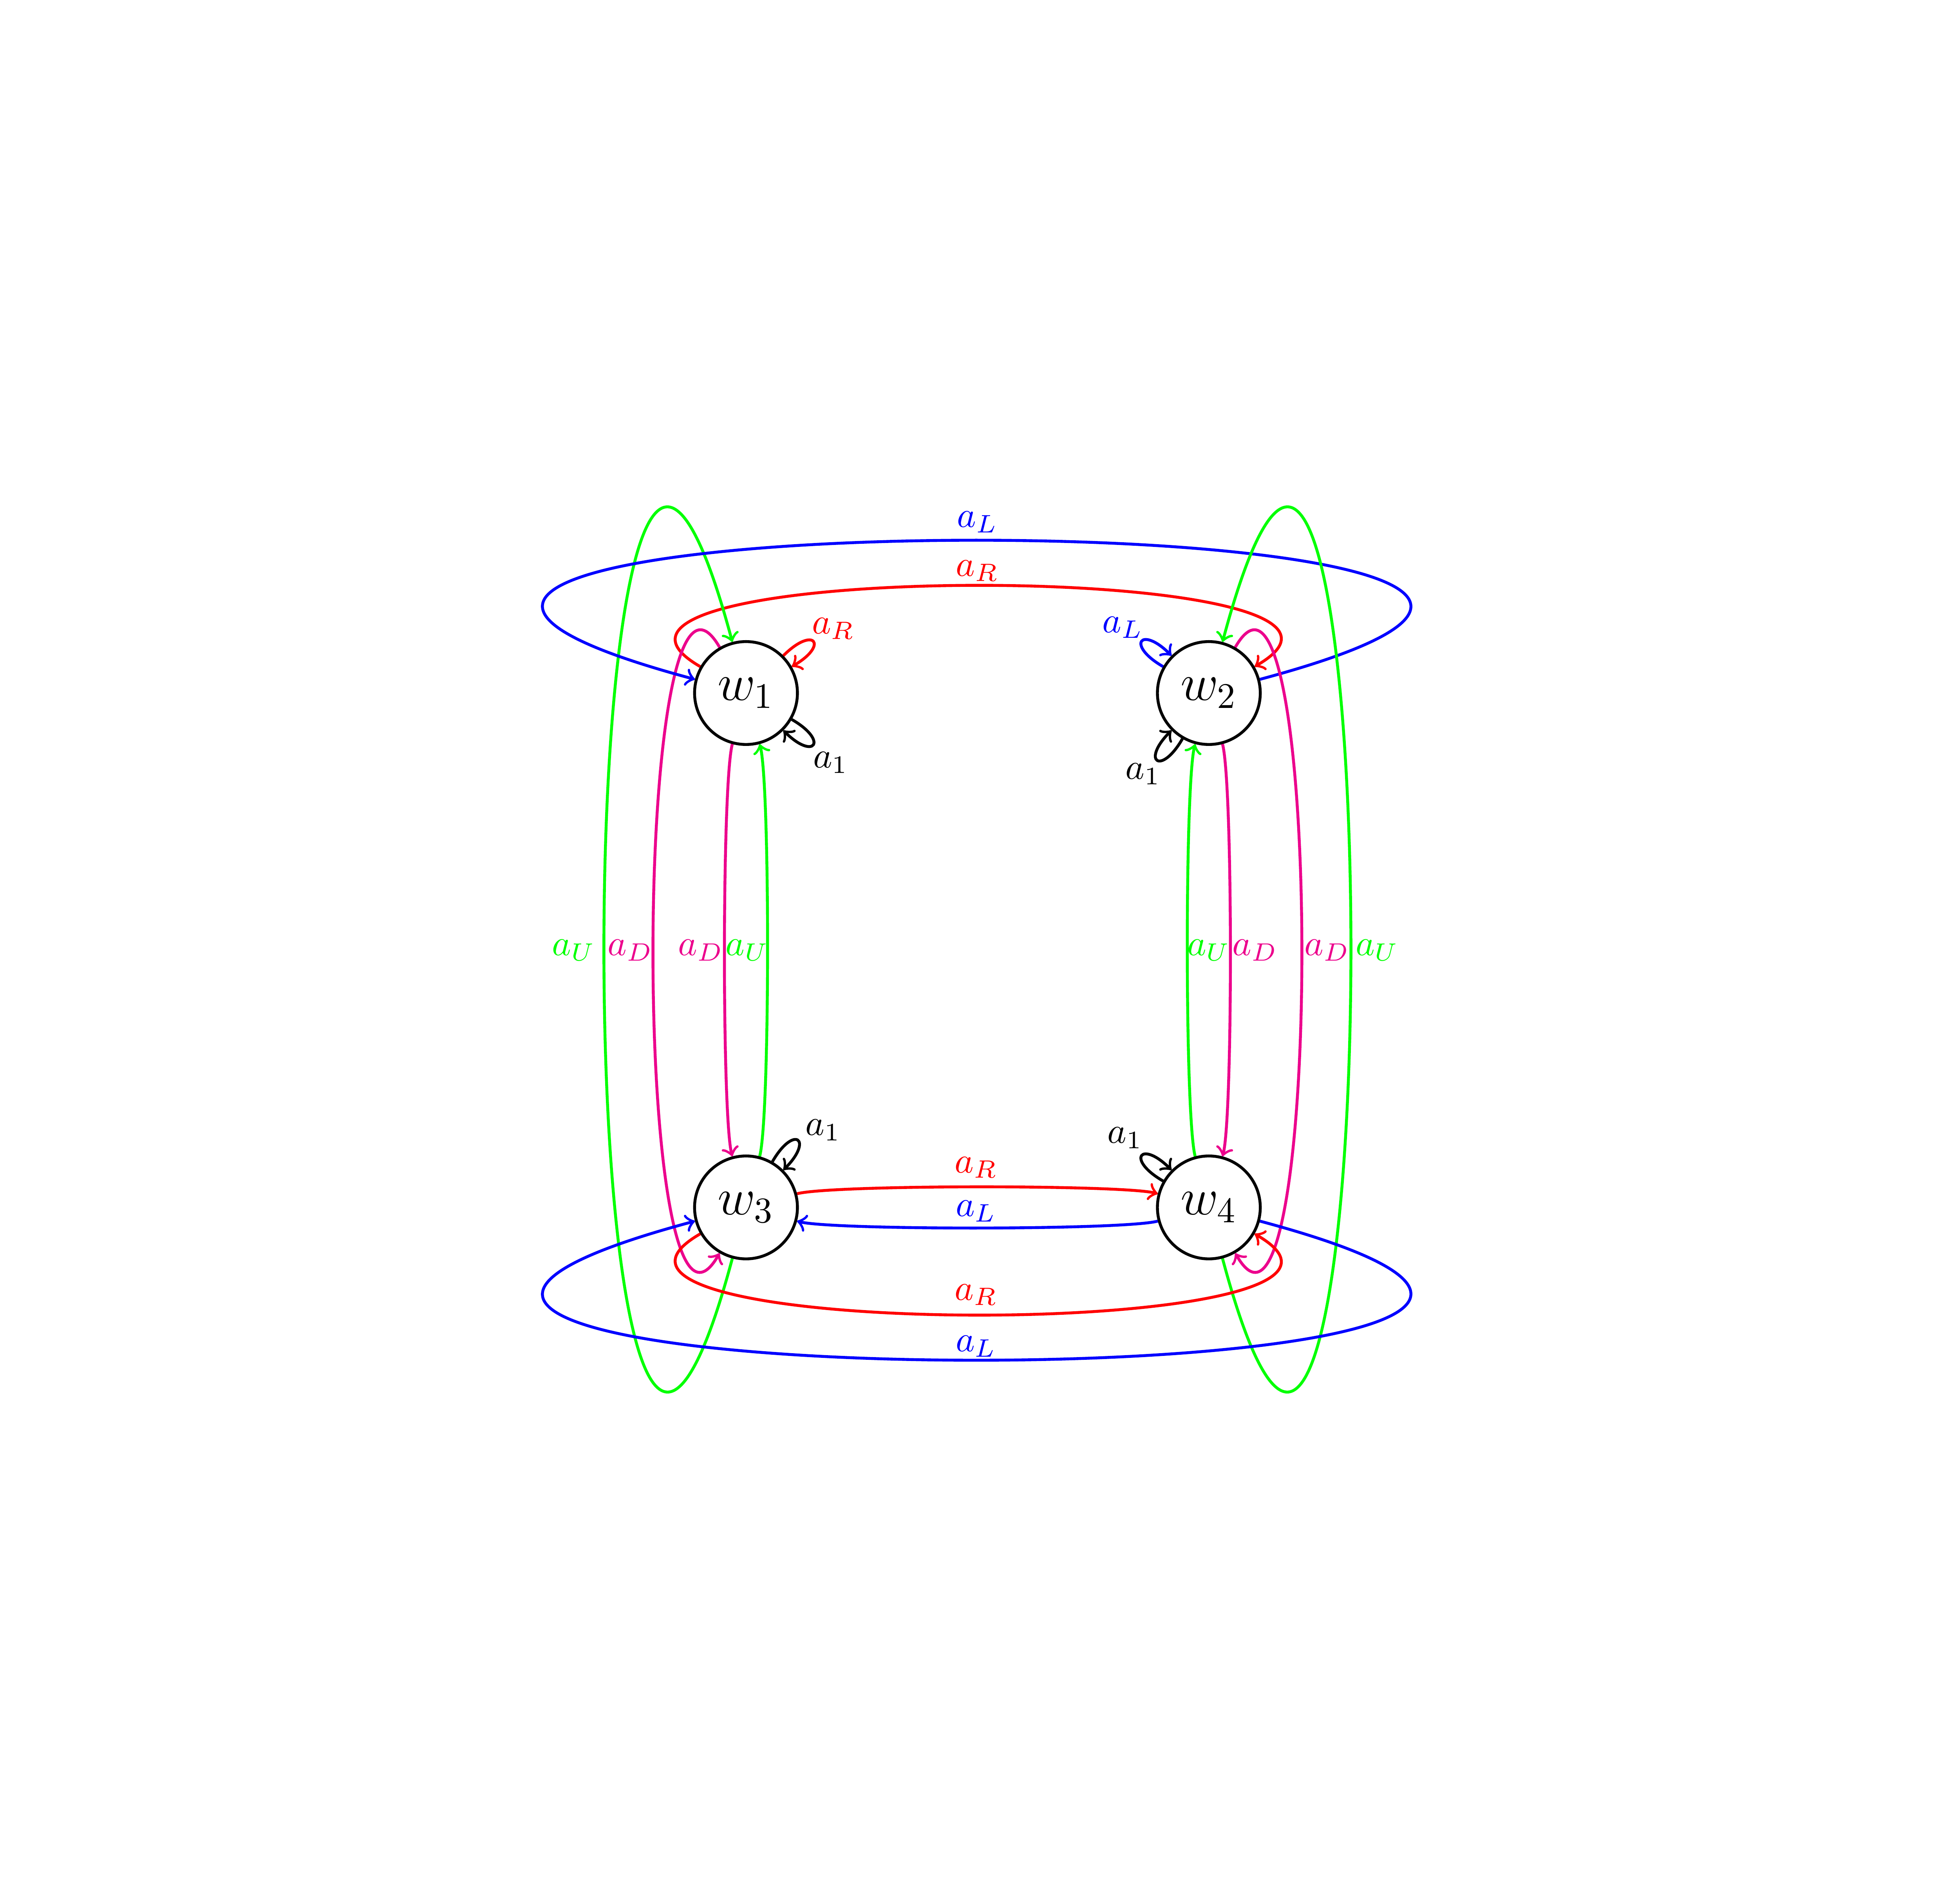
\includegraphics[width=0.75\linewidth]{5BeyondSBDRLGlobalAlgebras/Images/identity_walls_2x2_cyclical_min_actions.drawio.png}
    \caption{
        A world diagram of world $\mathscr{W}_{\beta}$ containing the labelled $\hat{D}_{A}$ transformations for an agent with minimum actions $\hat{A} = \{1, N, S, E, W\}$ using the identity treatment of constrained actions.
    }
    \label{fig:2x2_gridworld_minimum_transitions_wall_identity}
\end{figure}

\begin{table}[H]
\centering
\begin{tabular}{lc}
\hline
\textbf{Property} & \textbf{Present?} \\
\hline
Total & Y \\
Associative & Y \\
Identity & Y \\
Inverses & N \\
\hline
Commutative & N \\
\end{tabular}
\caption{
Group properties of $(\hat{A}^{*}/\sim, \circ_{\sim})$ for an agent with $\hat{A} = \{1, E, W, N, S \}$ in world $\mathscr{W}_{\beta}$ with identity treatment.
\draftnote{blue}{To do}{Sort table formatting.}
\draftnote{blue}{Consider}{Include Totality property ?}
}
\end{table}


\begin{fullwidth}
\begin{landscape}
\draftnote{blue}{To do}{
Figure out what to do with this table.
}
\setlength{\tabcolsep}{2pt}
{\fontsize{8}{10}\selectfont
\begin{longtable}[H]{l|llllllllllllllllllllllllll}
 & $1$ & $W$ & $N$ & $S$ & $NW$ & $SW$ & $WN$ & $NN$ & $SN$ & $WS$ & $WNW$ & $NNW$ & $SNW$ & $WSW$ & $NWN$ & $SWN$ & $WNN$ & $WSN$ & $NWS$ & $SWS$ & $NWNW$ & $SWNW$ & $WNNW$ & $WSNW$ & $NWSW$ & $SWSW$ \\
\midrule
\endfirsthead
 & $1$ & $W$ & $N$ & $S$ & $NW$ & $SW$ & $WN$ & $NN$ & $SN$ & $WS$ & $WNW$ & $NNW$ & $SNW$ & $WSW$ & $NWN$ & $SWN$ & $WNN$ & $WSN$ & $NWS$ & $SWS$ & $NWNW$ & $SWNW$ & $WNNW$ & $WSNW$ & $NWSW$ & $SWSW$ \\
\midrule
\endhead
\midrule
\multicolumn{27}{r}{Continued on next page} \\
\midrule
\endfoot
\endlastfoot
\textbf{$1$} & $1$ & $W$ & $N$ & $S$ & $NW$ & $SW$ & $WN$ & $NN$ & $SN$ & $WS$ & $WNW$ & $NNW$ & $SNW$ & $WSW$ & $NWN$ & $SWN$ & $WNN$ & $WSN$ & $NWS$ & $SWS$ & $NWNW$ & $SWNW$ & $WNNW$ & $WSNW$ & $NWSW$ & $SWSW$ \\
\textbf{$W$} & $W$ & $1$ & $WN$ & $WS$ & $WNW$ & $WSW$ & $N$ & $WNN$ & $WSN$ & $S$ & $NW$ & $WNNW$ & $WSNW$ & $SW$ & $SWSW$ & $SWNW$ & $NN$ & $SN$ & $NWSW$ & $NWNW$ & $SWS$ & $SWN$ & $NNW$ & $SNW$ & $NWS$ & $NWN$ \\
\textbf{$N$} & $N$ & $NW$ & $NN$ & $NN$ & $NNW$ & $NNW$ & $NWN$ & $N$ & $N$ & $NWS$ & $NWNW$ & $NW$ & $NW$ & $NWSW$ & $NWS$ & $NWS$ & $NWN$ & $NWS$ & $NWN$ & $NWN$ & $NWSW$ & $NWSW$ & $NWNW$ & $NWSW$ & $NWNW$ & $NWNW$ \\
\textbf{$S$} & $S$ & $SW$ & $SN$ & $SN$ & $SNW$ & $SNW$ & $SWN$ & $S$ & $S$ & $SWS$ & $SWNW$ & $SW$ & $SW$ & $SWSW$ & $SWS$ & $SWS$ & $SWN$ & $SWS$ & $SWN$ & $SWN$ & $SWSW$ & $SWSW$ & $SWNW$ & $SWSW$ & $SWNW$ & $SWNW$ \\
\textbf{$NW$} & $NW$ & $N$ & $NWN$ & $NWS$ & $NWNW$ & $NWSW$ & $NN$ & $NWN$ & $NWS$ & $NN$ & $NNW$ & $NWNW$ & $NWSW$ & $NNW$ & $NWNW$ & $NWSW$ & $N$ & $N$ & $NWNW$ & $NWSW$ & $NWN$ & $NWS$ & $NW$ & $NW$ & $NWN$ & $NWS$ \\
\textbf{$SW$} & $SW$ & $S$ & $SWN$ & $SWS$ & $SWNW$ & $SWSW$ & $SN$ & $SWN$ & $SWS$ & $SN$ & $SNW$ & $SWNW$ & $SWSW$ & $SNW$ & $SWNW$ & $SWSW$ & $S$ & $S$ & $SWNW$ & $SWSW$ & $SWN$ & $SWS$ & $SW$ & $SW$ & $SWN$ & $SWS$ \\
\textbf{$WN$} & $WN$ & $WNW$ & $WNN$ & $WNN$ & $WNNW$ & $WNNW$ & $SWSW$ & $WN$ & $WN$ & $NWSW$ & $SWS$ & $WNW$ & $WNW$ & $NWS$ & $NWSW$ & $NWSW$ & $SWSW$ & $NWSW$ & $SWSW$ & $SWSW$ & $NWS$ & $NWS$ & $SWS$ & $NWS$ & $SWS$ & $SWS$ \\
\textbf{$NN$} & $NN$ & $NNW$ & $N$ & $N$ & $NW$ & $NW$ & $NWS$ & $NN$ & $NN$ & $NWN$ & $NWSW$ & $NNW$ & $NNW$ & $NWNW$ & $NWN$ & $NWN$ & $NWS$ & $NWN$ & $NWS$ & $NWS$ & $NWNW$ & $NWNW$ & $NWSW$ & $NWNW$ & $NWSW$ & $NWSW$ \\
\textbf{$SN$} & $SN$ & $SNW$ & $S$ & $S$ & $SW$ & $SW$ & $SWS$ & $SN$ & $SN$ & $SWN$ & $SWSW$ & $SNW$ & $SNW$ & $SWNW$ & $SWN$ & $SWN$ & $SWS$ & $SWN$ & $SWS$ & $SWS$ & $SWNW$ & $SWNW$ & $SWSW$ & $SWNW$ & $SWSW$ & $SWSW$ \\
\textbf{$WS$} & $WS$ & $WSW$ & $WSN$ & $WSN$ & $WSNW$ & $WSNW$ & $SWNW$ & $WS$ & $WS$ & $NWNW$ & $SWN$ & $WSW$ & $WSW$ & $NWN$ & $NWNW$ & $NWNW$ & $SWNW$ & $NWNW$ & $SWNW$ & $SWNW$ & $NWN$ & $NWN$ & $SWN$ & $NWN$ & $SWN$ & $SWN$ \\
\textbf{$WNW$} & $WNW$ & $WN$ & $SWSW$ & $NWSW$ & $SWS$ & $NWS$ & $WNN$ & $SWSW$ & $NWSW$ & $WNN$ & $WNNW$ & $SWS$ & $NWS$ & $WNNW$ & $SWS$ & $NWS$ & $WN$ & $WN$ & $SWS$ & $NWS$ & $SWSW$ & $NWSW$ & $WNW$ & $WNW$ & $SWSW$ & $NWSW$ \\
\textbf{$NNW$} & $NNW$ & $NN$ & $NWS$ & $NWN$ & $NWSW$ & $NWNW$ & $N$ & $NWS$ & $NWN$ & $N$ & $NW$ & $NWSW$ & $NWNW$ & $NW$ & $NWSW$ & $NWNW$ & $NN$ & $NN$ & $NWSW$ & $NWNW$ & $NWS$ & $NWN$ & $NNW$ & $NNW$ & $NWS$ & $NWN$ \\
\textbf{$SNW$} & $SNW$ & $SN$ & $SWS$ & $SWN$ & $SWSW$ & $SWNW$ & $S$ & $SWS$ & $SWN$ & $S$ & $SW$ & $SWSW$ & $SWNW$ & $SW$ & $SWSW$ & $SWNW$ & $SN$ & $SN$ & $SWSW$ & $SWNW$ & $SWS$ & $SWN$ & $SNW$ & $SNW$ & $SWS$ & $SWN$ \\
\textbf{$WSW$} & $WSW$ & $WS$ & $SWNW$ & $NWNW$ & $SWN$ & $NWN$ & $WSN$ & $SWNW$ & $NWNW$ & $WSN$ & $WSNW$ & $SWN$ & $NWN$ & $WSNW$ & $SWN$ & $NWN$ & $WS$ & $WS$ & $SWN$ & $NWN$ & $SWNW$ & $NWNW$ & $WSW$ & $WSW$ & $SWNW$ & $NWNW$ \\
\textbf{$NWN$} & $NWN$ & $NWNW$ & $NWN$ & $NWN$ & $NWNW$ & $NWNW$ & $NWNW$ & $NWN$ & $NWN$ & $NWNW$ & $NWN$ & $NWNW$ & $NWNW$ & $NWN$ & $NWNW$ & $NWNW$ & $NWNW$ & $NWNW$ & $NWNW$ & $NWNW$ & $NWN$ & $NWN$ & $NWN$ & $NWN$ & $NWN$ & $NWN$ \\
\textbf{$SWN$} & $SWN$ & $SWNW$ & $SWN$ & $SWN$ & $SWNW$ & $SWNW$ & $SWNW$ & $SWN$ & $SWN$ & $SWNW$ & $SWN$ & $SWNW$ & $SWNW$ & $SWN$ & $SWNW$ & $SWNW$ & $SWNW$ & $SWNW$ & $SWNW$ & $SWNW$ & $SWN$ & $SWN$ & $SWN$ & $SWN$ & $SWN$ & $SWN$ \\
\textbf{$WNN$} & $WNN$ & $WNNW$ & $WN$ & $WN$ & $WNW$ & $WNW$ & $NWSW$ & $WNN$ & $WNN$ & $SWSW$ & $NWS$ & $WNNW$ & $WNNW$ & $SWS$ & $SWSW$ & $SWSW$ & $NWSW$ & $SWSW$ & $NWSW$ & $NWSW$ & $SWS$ & $SWS$ & $NWS$ & $SWS$ & $NWS$ & $NWS$ \\
\textbf{$WSN$} & $WSN$ & $WSNW$ & $WS$ & $WS$ & $WSW$ & $WSW$ & $NWNW$ & $WSN$ & $WSN$ & $SWNW$ & $NWN$ & $WSNW$ & $WSNW$ & $SWN$ & $SWNW$ & $SWNW$ & $NWNW$ & $SWNW$ & $NWNW$ & $NWNW$ & $SWN$ & $SWN$ & $NWN$ & $SWN$ & $NWN$ & $NWN$ \\
\textbf{$NWS$} & $NWS$ & $NWSW$ & $NWS$ & $NWS$ & $NWSW$ & $NWSW$ & $NWSW$ & $NWS$ & $NWS$ & $NWSW$ & $NWS$ & $NWSW$ & $NWSW$ & $NWS$ & $NWSW$ & $NWSW$ & $NWSW$ & $NWSW$ & $NWSW$ & $NWSW$ & $NWS$ & $NWS$ & $NWS$ & $NWS$ & $NWS$ & $NWS$ \\
\textbf{$SWS$} & $SWS$ & $SWSW$ & $SWS$ & $SWS$ & $SWSW$ & $SWSW$ & $SWSW$ & $SWS$ & $SWS$ & $SWSW$ & $SWS$ & $SWSW$ & $SWSW$ & $SWS$ & $SWSW$ & $SWSW$ & $SWSW$ & $SWSW$ & $SWSW$ & $SWSW$ & $SWS$ & $SWS$ & $SWS$ & $SWS$ & $SWS$ & $SWS$ \\
\textbf{$NWNW$} & $NWNW$ & $NWN$ & $NWNW$ & $NWNW$ & $NWN$ & $NWN$ & $NWN$ & $NWNW$ & $NWNW$ & $NWN$ & $NWNW$ & $NWN$ & $NWN$ & $NWNW$ & $NWN$ & $NWN$ & $NWN$ & $NWN$ & $NWN$ & $NWN$ & $NWNW$ & $NWNW$ & $NWNW$ & $NWNW$ & $NWNW$ & $NWNW$ \\
\textbf{$SWNW$} & $SWNW$ & $SWN$ & $SWNW$ & $SWNW$ & $SWN$ & $SWN$ & $SWN$ & $SWNW$ & $SWNW$ & $SWN$ & $SWNW$ & $SWN$ & $SWN$ & $SWNW$ & $SWN$ & $SWN$ & $SWN$ & $SWN$ & $SWN$ & $SWN$ & $SWNW$ & $SWNW$ & $SWNW$ & $SWNW$ & $SWNW$ & $SWNW$ \\
\textbf{$WNNW$} & $WNNW$ & $WNN$ & $NWSW$ & $SWSW$ & $NWS$ & $SWS$ & $WN$ & $NWSW$ & $SWSW$ & $WN$ & $WNW$ & $NWS$ & $SWS$ & $WNW$ & $NWS$ & $SWS$ & $WNN$ & $WNN$ & $NWS$ & $SWS$ & $NWSW$ & $SWSW$ & $WNNW$ & $WNNW$ & $NWSW$ & $SWSW$ \\
\textbf{$WSNW$} & $WSNW$ & $WSN$ & $NWNW$ & $SWNW$ & $NWN$ & $SWN$ & $WS$ & $NWNW$ & $SWNW$ & $WS$ & $WSW$ & $NWN$ & $SWN$ & $WSW$ & $NWN$ & $SWN$ & $WSN$ & $WSN$ & $NWN$ & $SWN$ & $NWNW$ & $SWNW$ & $WSNW$ & $WSNW$ & $NWNW$ & $SWNW$ \\
\textbf{$NWSW$} & $NWSW$ & $NWS$ & $NWSW$ & $NWSW$ & $NWS$ & $NWS$ & $NWS$ & $NWSW$ & $NWSW$ & $NWS$ & $NWSW$ & $NWS$ & $NWS$ & $NWSW$ & $NWS$ & $NWS$ & $NWS$ & $NWS$ & $NWS$ & $NWS$ & $NWSW$ & $NWSW$ & $NWSW$ & $NWSW$ & $NWSW$ & $NWSW$ \\
\textbf{$SWSW$} & $SWSW$ & $SWS$ & $SWSW$ & $SWSW$ & $SWS$ & $SWS$ & $SWS$ & $SWSW$ & $SWSW$ & $SWS$ & $SWSW$ & $SWS$ & $SWS$ & $SWSW$ & $SWS$ & $SWS$ & $SWS$ & $SWS$ & $SWS$ & $SWS$ & $SWSW$ & $SWSW$ & $SWSW$ & $SWSW$ & $SWSW$ & $SWSW$ \\
\caption{Insert caption here}
\end{longtable}

}
\setlength{\tabcolsep}{6pt}
\end{landscape}
\end{fullwidth}


%%%%%%%%%%%%%%%%%%%%%%%%%%%%%%%%%%%%%%%%%%%%%
\subsection{Analysis}

\begin{table}[H]
    \centering
    \begin{tabular}{lc}
    \hline
        \textbf{World} & \bm{$|\hat{A}^{*}/\sim|$} \\
        \hline
        $\mathscr{W}_{\alpha}$ & 4 \\
        $\mathscr{W}_{\beta}$ with masked treatment & 59 \\
        $\mathscr{W}_{\beta}$ with identity treatment & 26
    \end{tabular}
    \caption{
    Comparison of the number of elements in the transformation algebras of the $2 \times 2$ gridworld world without a wall $\mathscr{W}_{\alpha}$ and with a wall $\mathscr{W}_{\beta}$.
    \draftnote{blue}{To do}{Rewrite caption.}
    }
    \label{tab:num_elements_comparision_2x2_gridworlds}
\end{table}

As we can see from \cref{tab:num_elements_comparision_2x2_gridworlds}, adding a single wall to the world $\mathscr{W}_{\alpha}$ has massively increased the complexity of the transformation algebra of the world.
Adding the wall has broken the symmetry of the world $\mathscr{W}_{\alpha}$
\draftnote{blue}{To do}{
Check this + check for subgroups (perhaps symmetry only broken in the $E$-$W$ direction.
}
.

\begin{proposition}
    The algebra $\hat{A}^{*}/\sim$ of the transformations due to the actions of an agent depends on the treatment of constrained actions in the same world.
\end{proposition}
\begin{proof}
    \textbf{Proof by example.}
    Consider the world $\mathscr{W}_{\beta}$.
    From \cref{tab:num_elements_comparision_2x2_gridworlds}, we can see that the algebras $\hat{A}^{*}/\sim$ for the world $\mathscr{W}_{\beta}$ where different treatments of constrained actions have been used are not isomorphic because isomorphic algebras must contain the same number of elements.
\end{proof}

%%%%%%%%%%%%%%%%%%%%%%%%%%%%%%%%%%%%%%%%%%%%%
\section{Reversible worlds}

\draftnote{green}{To do}{
\begin{enumerate}
    \item Proof: constrained actions are inhomogeneous actions. (do after inhomogeneous actions introduced)
    \item 
\end{enumerate}
}

We will now consider worlds where every action is reversible; we call these \emph{reversible worlds}.
We have already seen two examples of reversible worlds: $\mathscr{W}_{\alpha}$ and $\mathscr{W}_{\beta}$ with the identity treatment.

\draftnote{blue}{awjdean}{Example of reversible action-inhomogeneous world with no constrained actions}
Consider a world $\mathscr{W}_{\gamma}$ with movement of an agent along a single 1D cyclical axis with a movable block (world states in \cref{fig:movable_block_world_states}).
If the agent is in the location directly to the left of the block and moves into the block, the block moves one location in the direction of the agent's movement and the agent moves into the location previously occupied by the block (see \cref{tab:4x1_gridworld_min_transitions_moveable_block,fig:4x1_block_min_actions_wall}).

\begin{figure}[H]
  \centering
  \begin{subfigure}{0.48\textwidth}
    \centering
    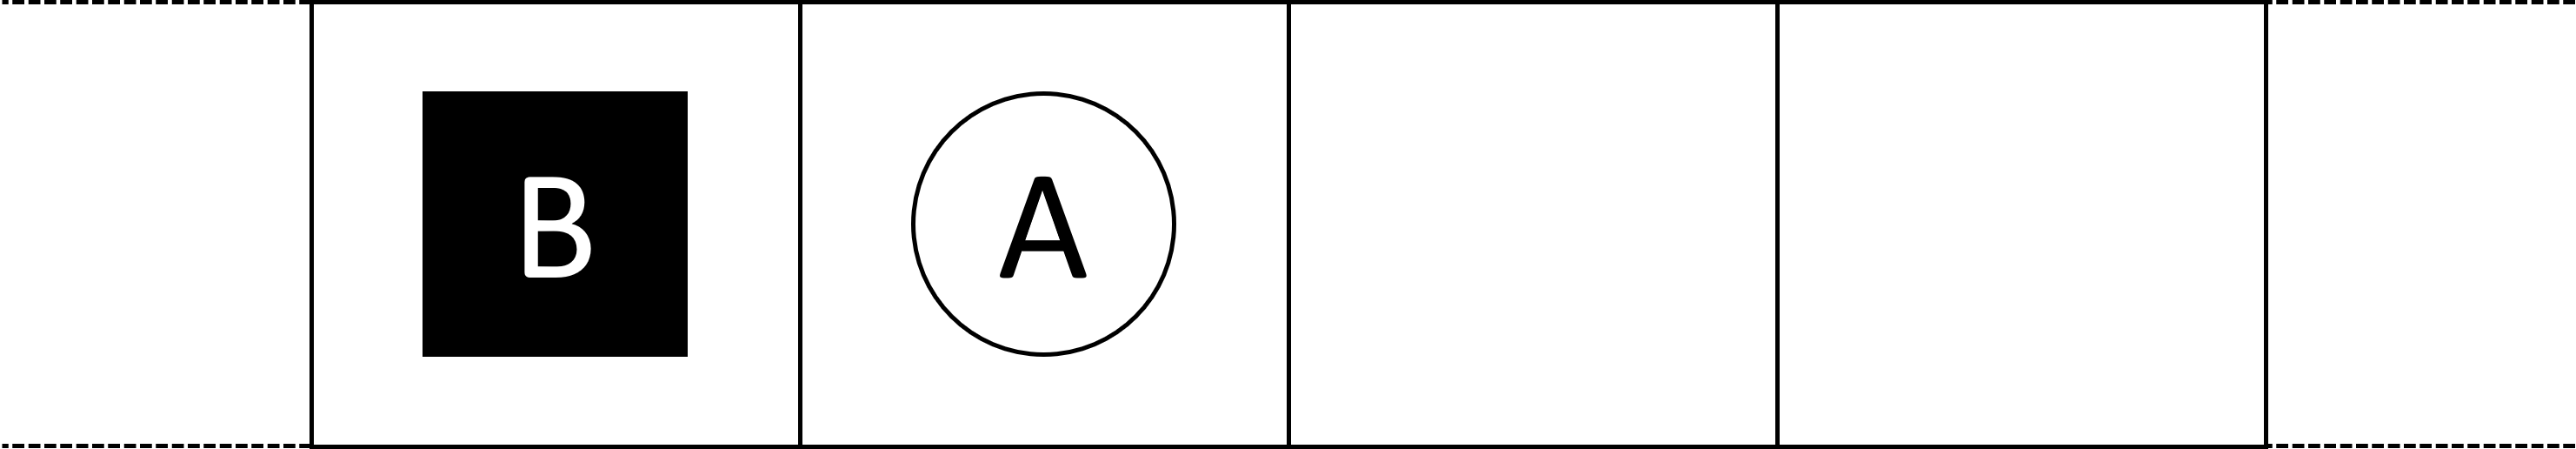
\includegraphics[width=\textwidth]{5BeyondSBDRLGlobalAlgebras/Images/Movable_block_world_states/w0.png}
    \caption{$w_{0}$}
  \end{subfigure}%
  \hfill
  \begin{subfigure}{0.48\textwidth}
    \centering
    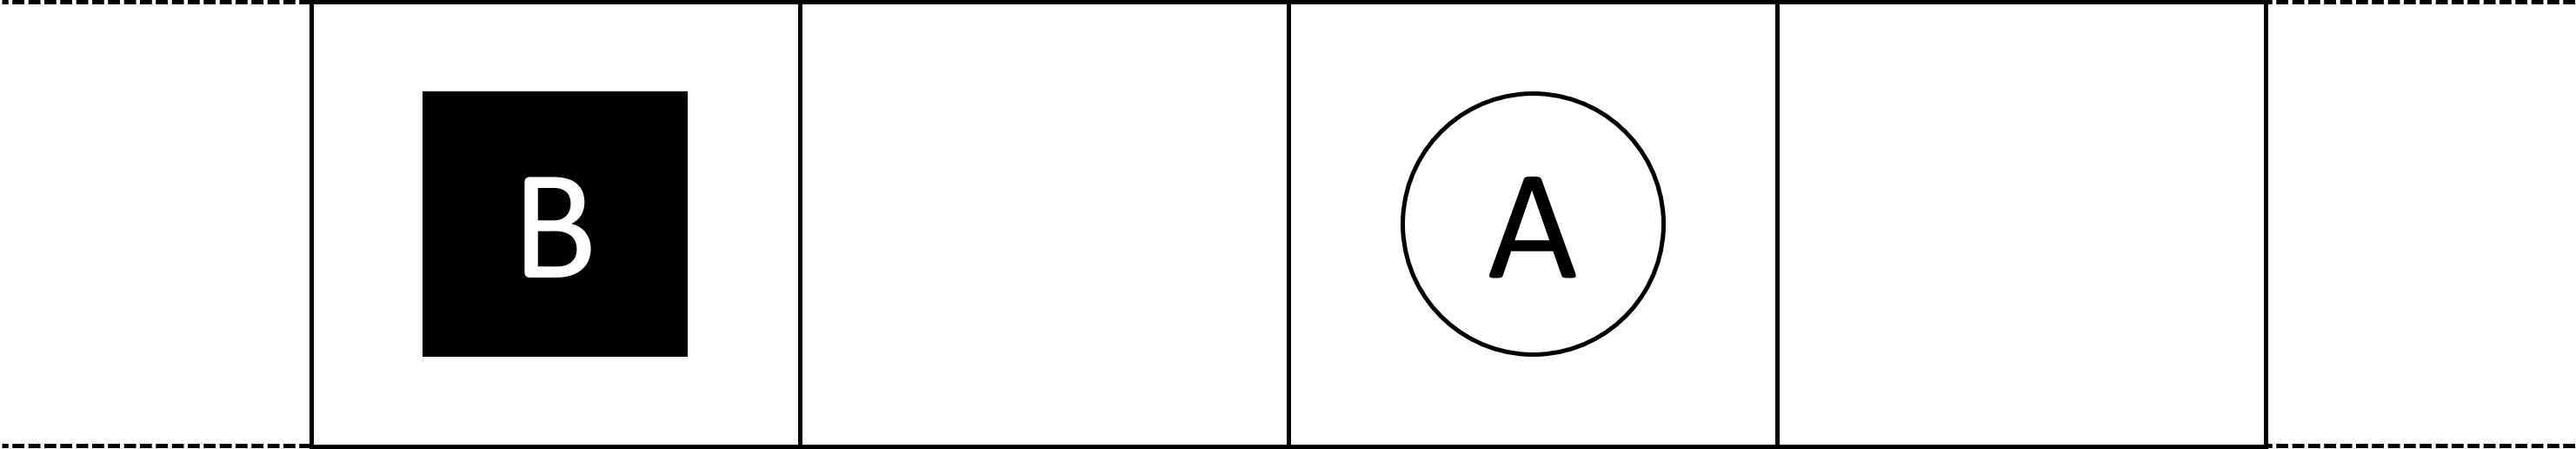
\includegraphics[width=\textwidth]{5BeyondSBDRLGlobalAlgebras/Images/Movable_block_world_states/w1.png}
    \caption{$w_{1}$}
  \end{subfigure}%
  \vspace{0.5cm}
  \begin{subfigure}{0.48\textwidth}
    \centering
    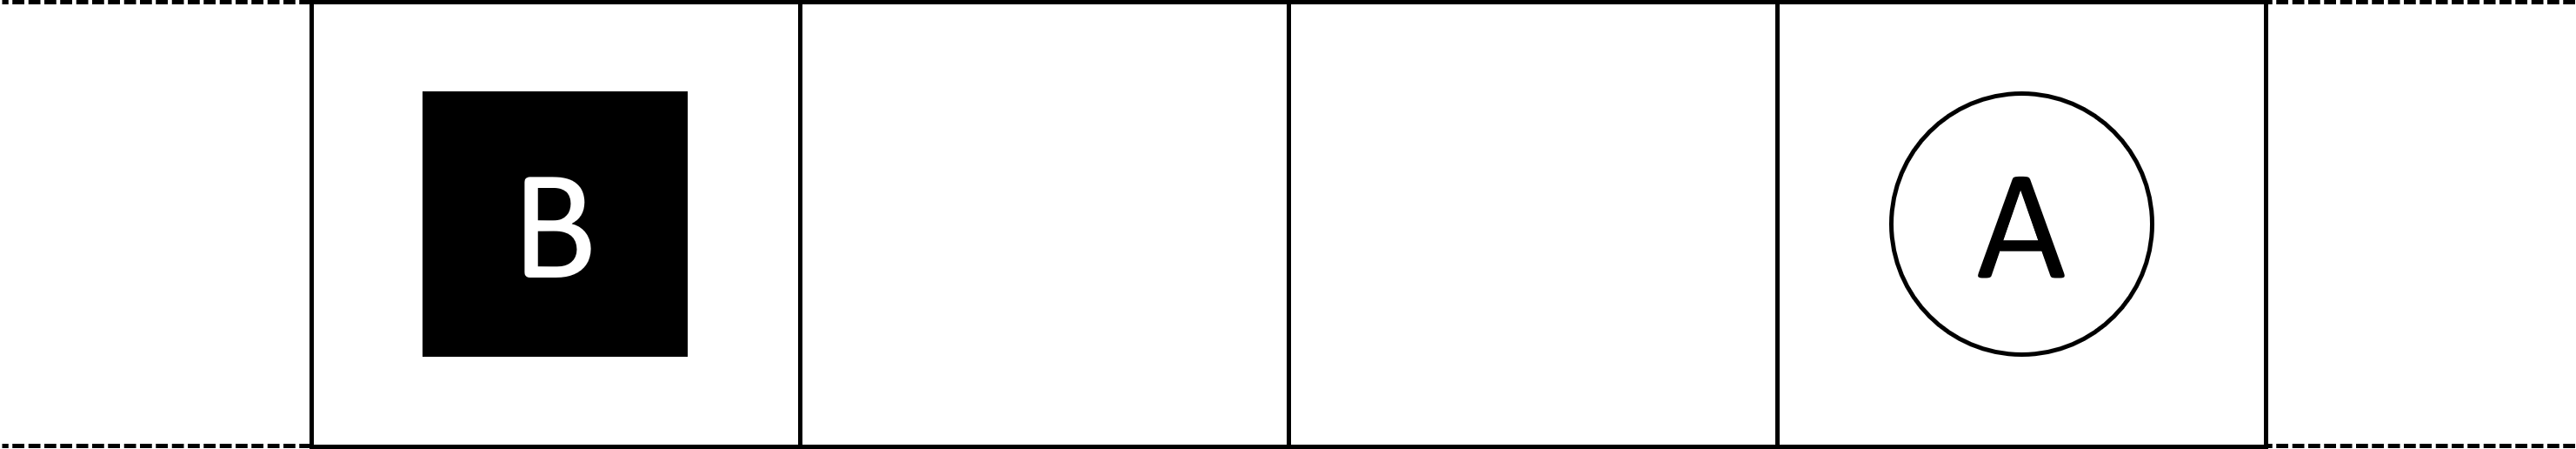
\includegraphics[width=\textwidth]{5BeyondSBDRLGlobalAlgebras/Images/Movable_block_world_states/w2.png}
    \caption{$w_{2}$}
  \end{subfigure}%
  \hfill
  \begin{subfigure}{0.48\textwidth}
    \centering
    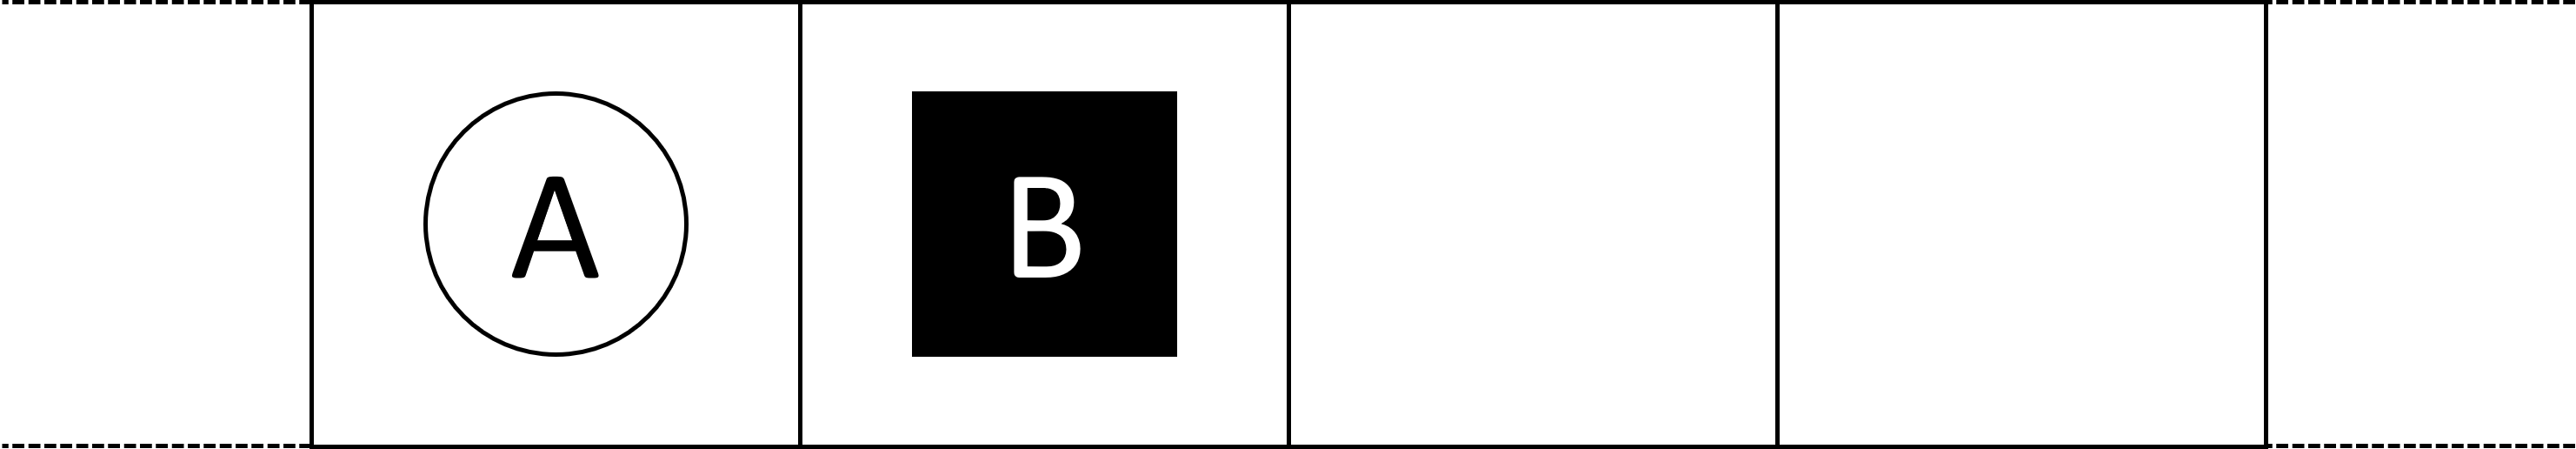
\includegraphics[width=\textwidth]{5BeyondSBDRLGlobalAlgebras/Images/Movable_block_world_states/w3.png}
    \caption{$w_{3}$}
  \end{subfigure}%
  \vspace{0.5cm}
  \begin{subfigure}{0.48\textwidth}
    \centering
    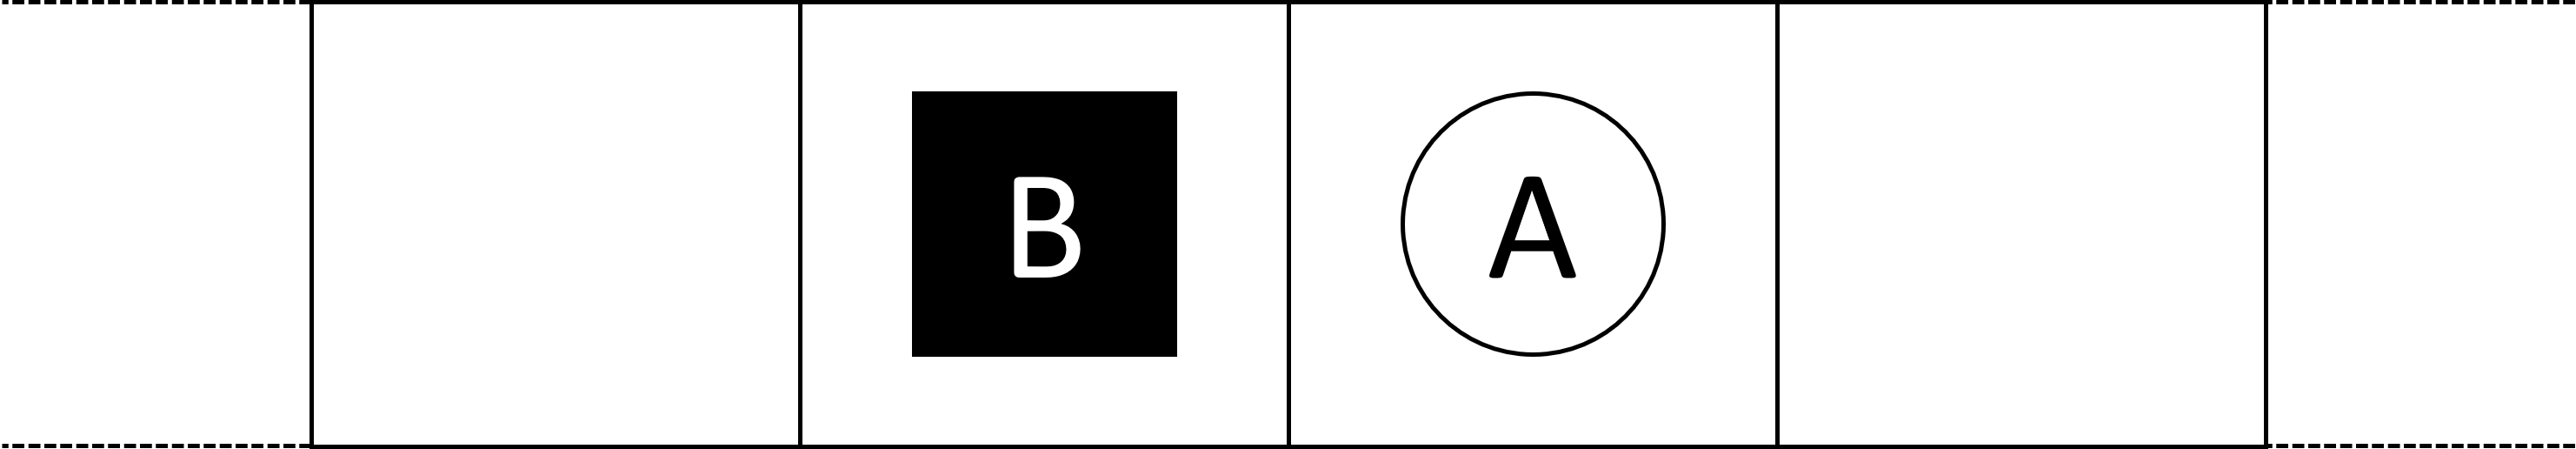
\includegraphics[width=\textwidth]{5BeyondSBDRLGlobalAlgebras/Images/Movable_block_world_states/w4.png}
    \caption{$w_{4}$}
  \end{subfigure}%
  \hfill
  \begin{subfigure}{0.48\textwidth}
    \centering
    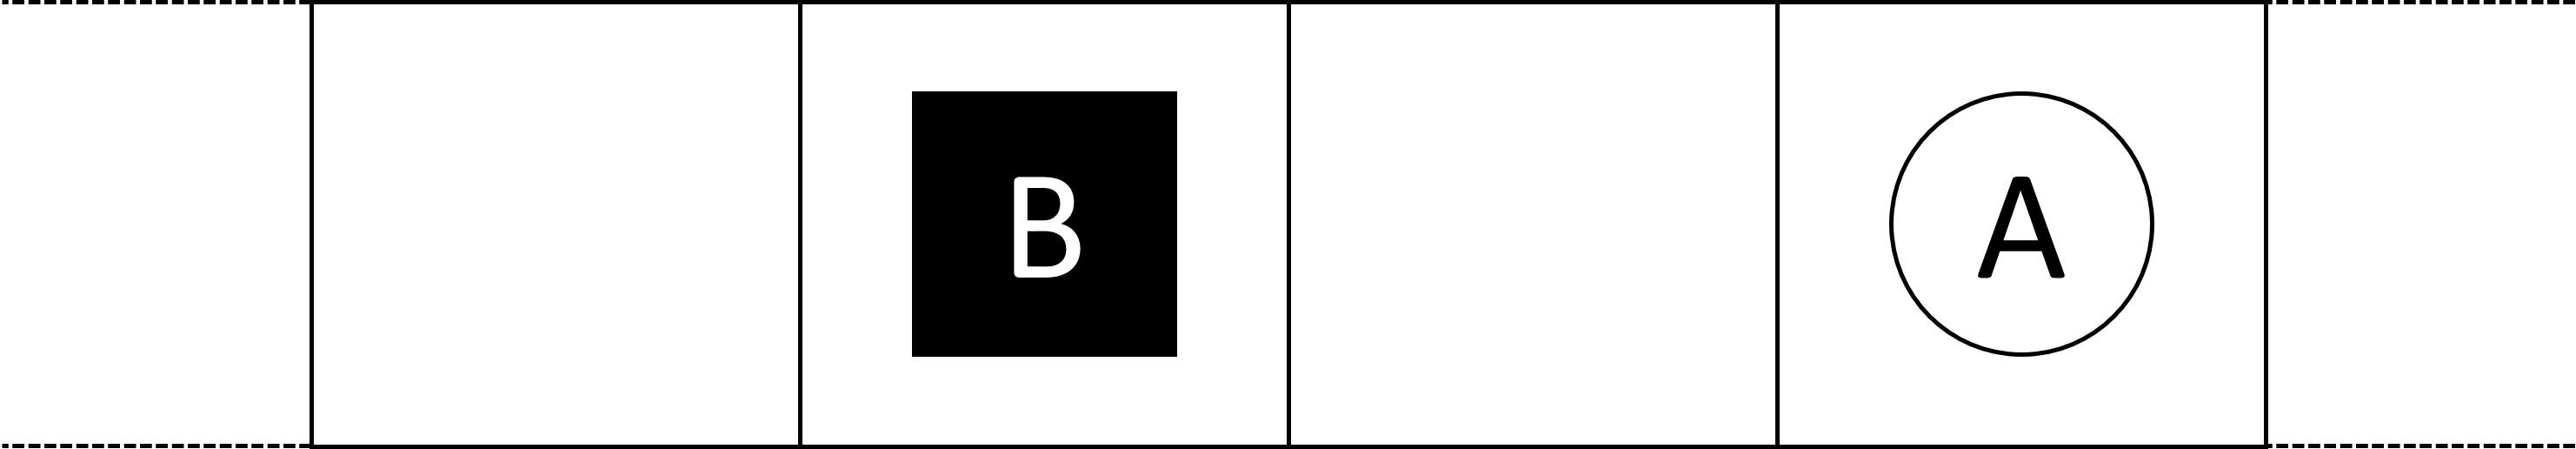
\includegraphics[width=\textwidth]{5BeyondSBDRLGlobalAlgebras/Images/Movable_block_world_states/w5.png}
    \caption{$w_{5}$}
  \end{subfigure}%
  \vspace{0.5cm}
  \begin{subfigure}{0.48\textwidth}
    \centering
    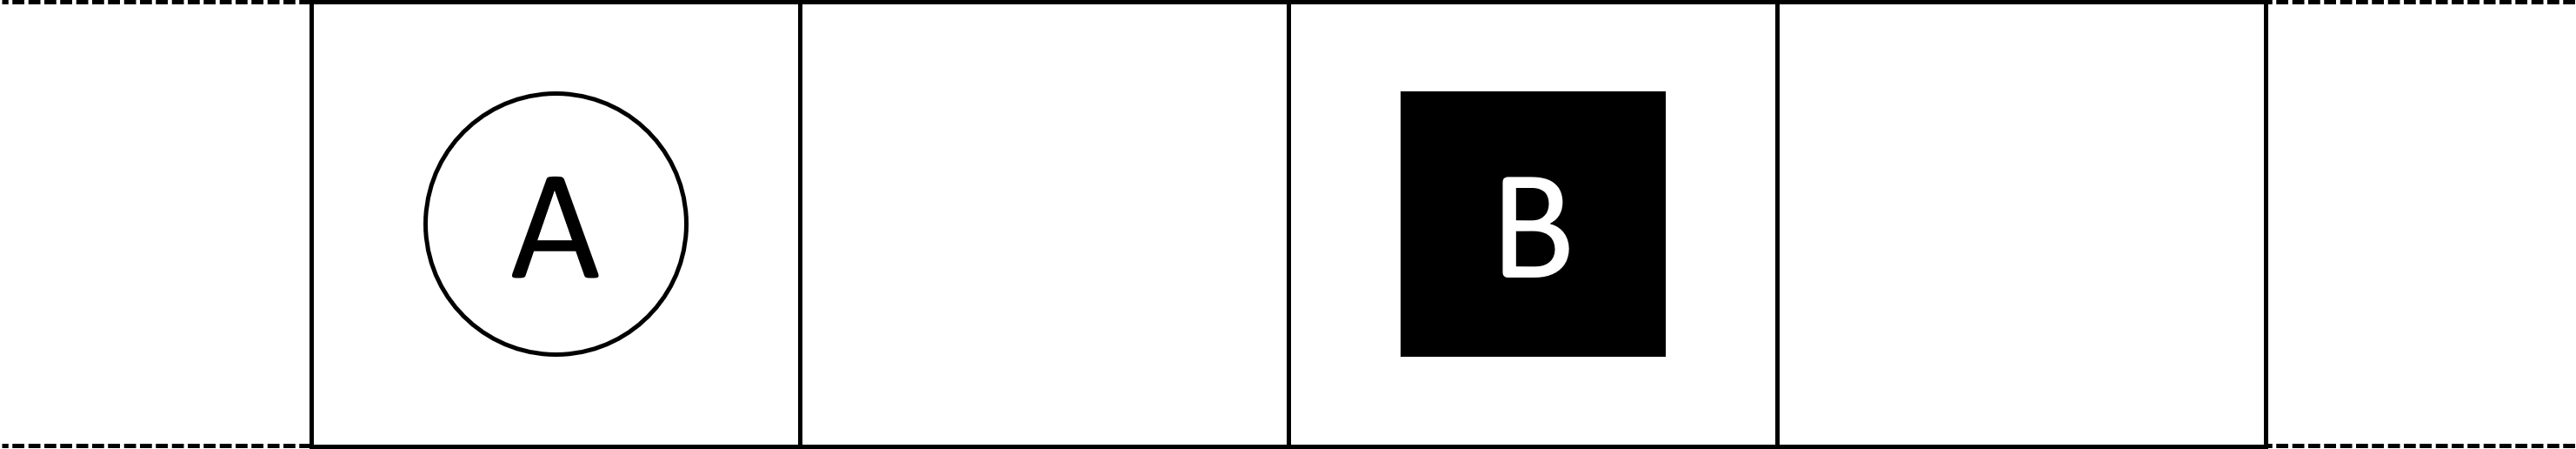
\includegraphics[width=\textwidth]{5BeyondSBDRLGlobalAlgebras/Images/Movable_block_world_states/w6.png}
    \caption{$w_{6}$}
  \end{subfigure}%
  \hfill
  \begin{subfigure}{0.48\textwidth}
    \centering
    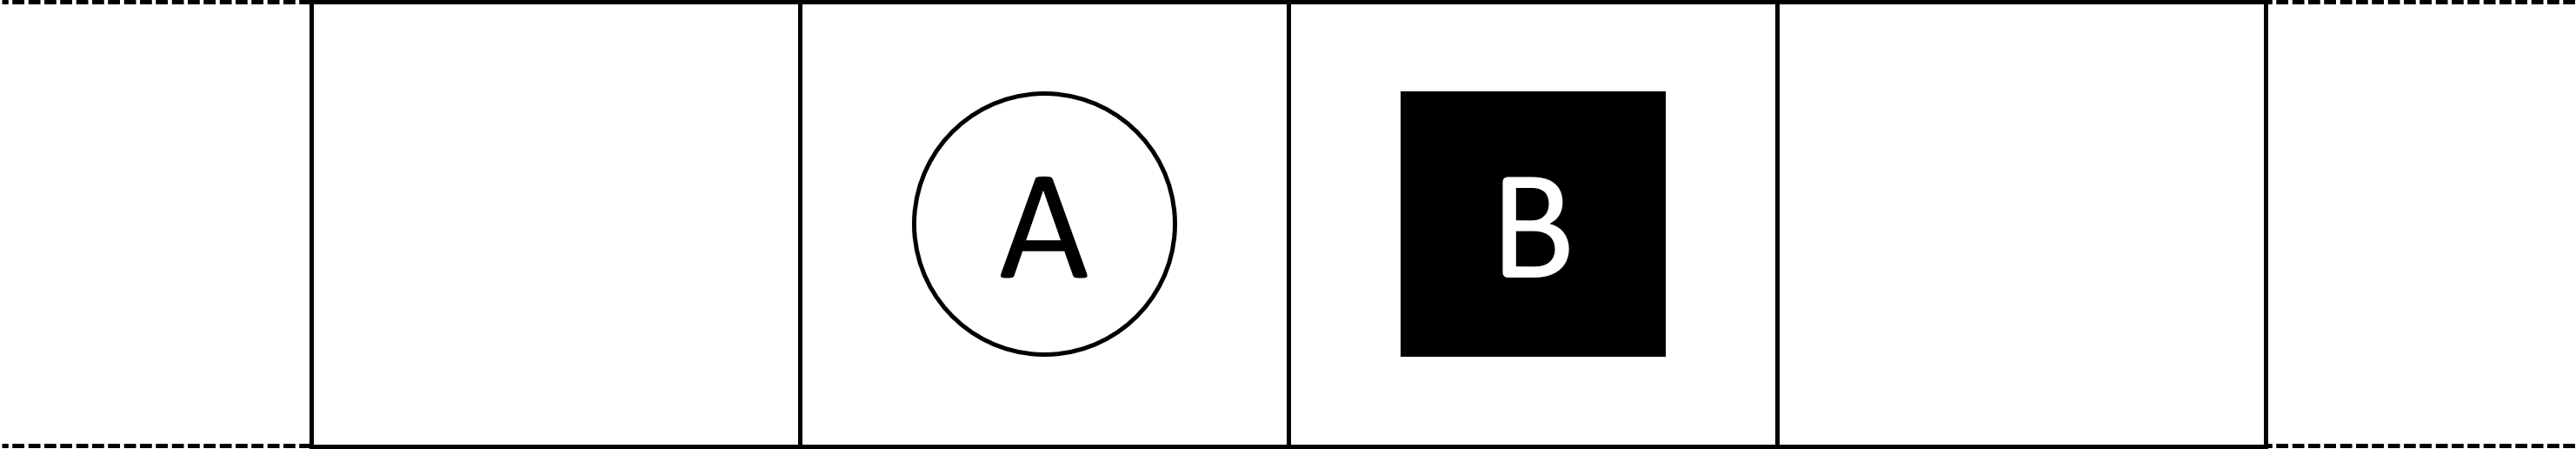
\includegraphics[width=\textwidth]{5BeyondSBDRLGlobalAlgebras/Images/Movable_block_world_states/w7.png}
    \caption{$w_{7}$}
  \end{subfigure}%
  \vspace{0.5cm}
  \begin{subfigure}{0.48\textwidth}
    \centering
    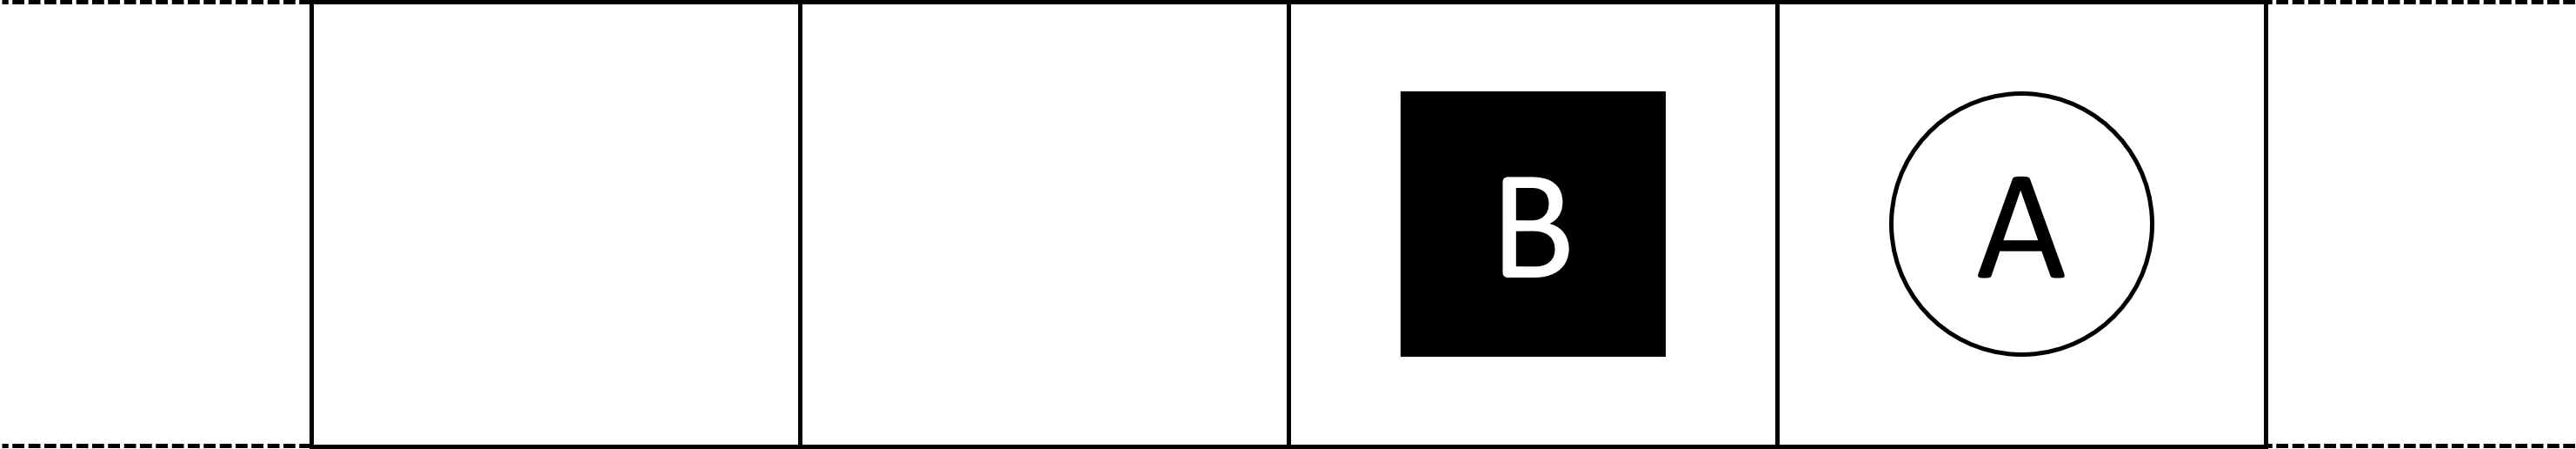
\includegraphics[width=\textwidth]{5BeyondSBDRLGlobalAlgebras/Images/Movable_block_world_states/w8.png}
    \caption{$w_{8}$}
  \end{subfigure}%
  \hfill
  \begin{subfigure}{0.48\textwidth}
    \centering
    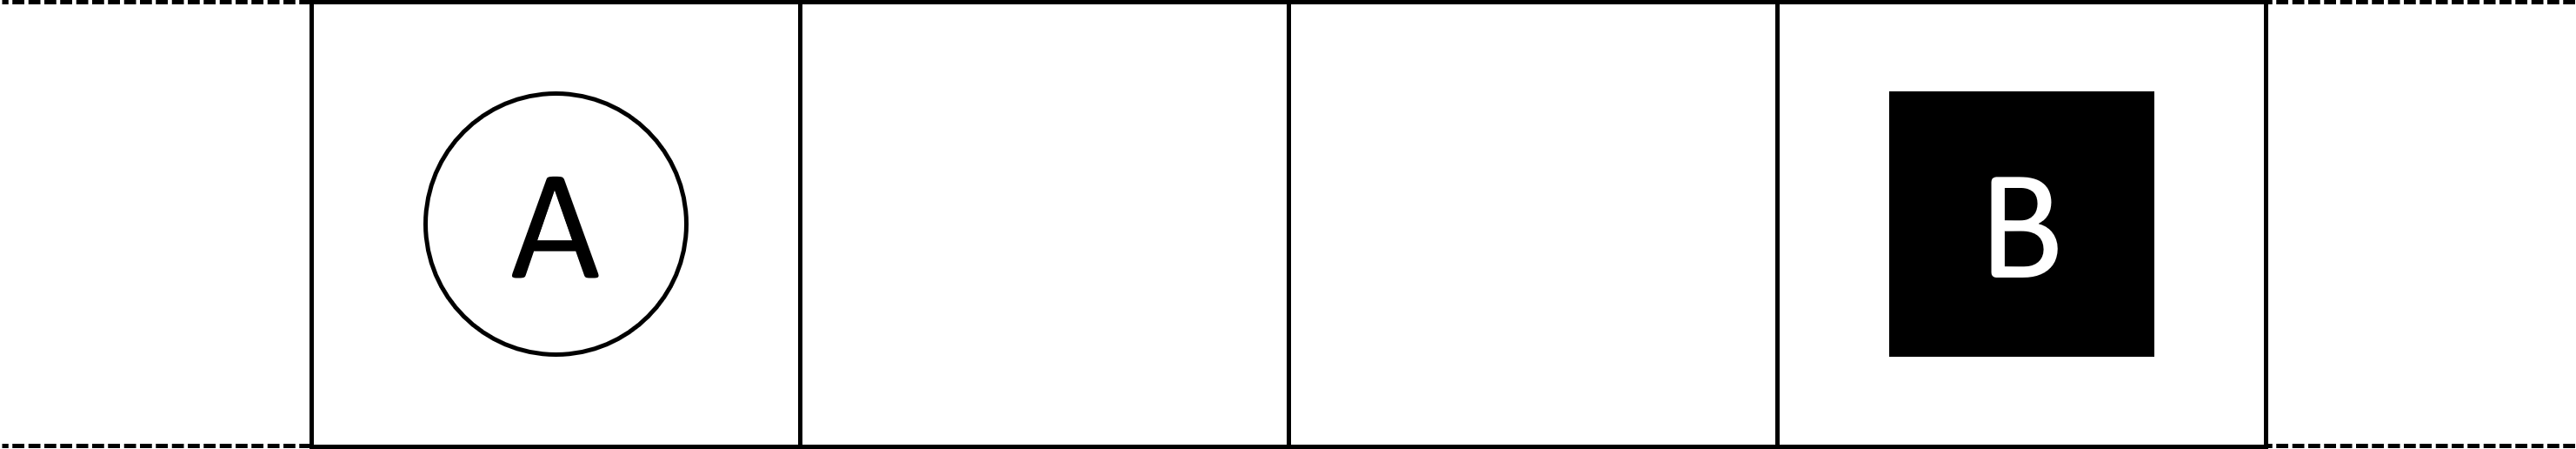
\includegraphics[width=\textwidth]{5BeyondSBDRLGlobalAlgebras/Images/Movable_block_world_states/w9.png}
    \caption{$w_{9}$}
  \end{subfigure}%
    \vspace{0.5cm}
  \begin{subfigure}{0.48\textwidth}
    \centering
    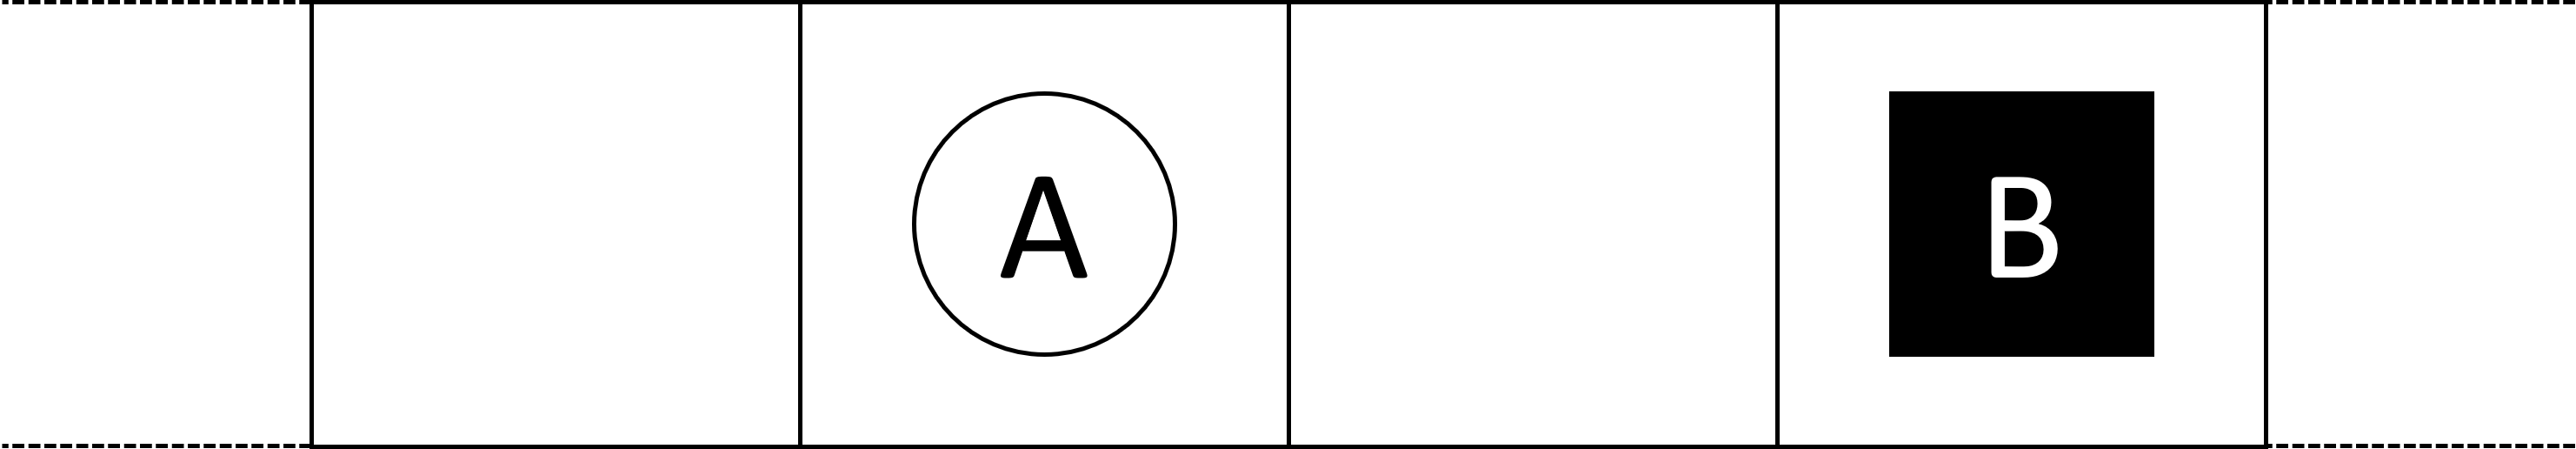
\includegraphics[width=\textwidth]{5BeyondSBDRLGlobalAlgebras/Images/Movable_block_world_states/w10.png}
    \caption{$w_{10}$}
  \end{subfigure}%
  \hfill
  \begin{subfigure}{0.48\textwidth}
    \centering
    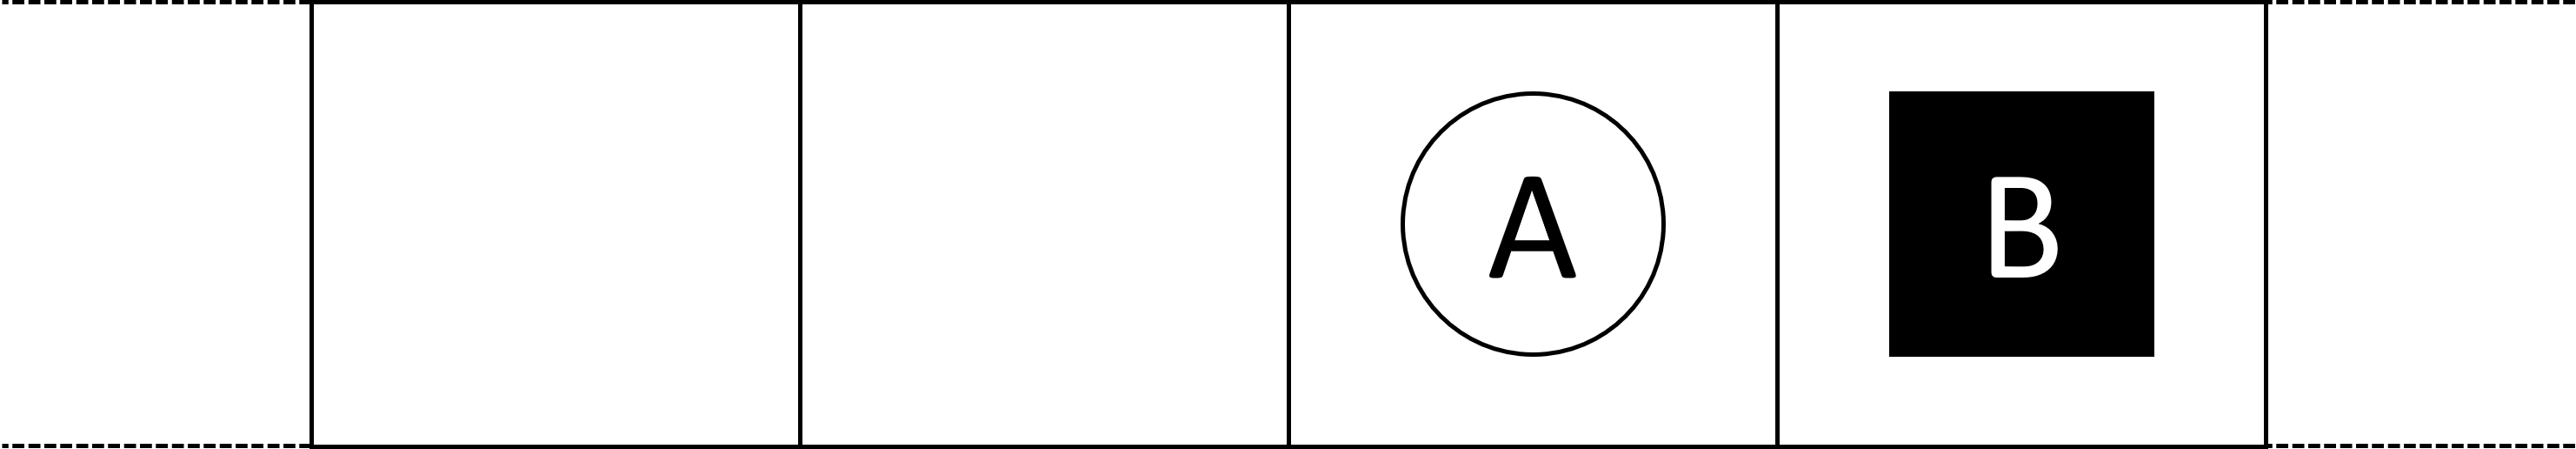
\includegraphics[width=\textwidth]{5BeyondSBDRLGlobalAlgebras/Images/Movable_block_world_states/w11.png}
    \caption{$w_{11}$}
  \end{subfigure}%
  \caption{World states of the world $\mathscr{W}_{\gamma}$ containing an agent and a movable block.}
  \label{fig:movable_block_world_states}
\end{figure}

\begin{table}[H]
    \centering
    \begin{tabular}{c|c c c c c}
                &  $1$      & $L$      & $R$\\
         \hline
        $w_{0}$ & $w_{0}$   & $w_{9}$   & $w_{1}$\\
        $w_{1}$ & $w_{1}$   & $w_{0}$   & $w_{2}$\\
        $w_{2}$ & $w_{2}$   & $w_{1}$   & $w_{3}$\\
        $w_{3}$ & $w_{3}$   & $w_{5}$   & $w_{7}$\\
        $w_{4}$ & $w_{4}$   & $w_{0}$   & $w_{5}$\\
        $w_{5}$ & $w_{5}$   & $w_{4}$   & $w_{3}$\\
        $w_{6}$ & $w_{6}$   & $w_{8}$   & $w_{7}$\\
        $w_{7}$ & $w_{7}$   & $w_{6}$   & $w_{11}$\\
        $w_{8}$ & $w_{8}$   & $w_{4}$   & $w_{6}$\\
        $w_{9}$ & $w_{9}$   & $w_{8}$   & $w_{10}$\\
        $w_{10}$ & $w_{10}$ & $w_{9}$   & $w_{11}$\\
        $w_{11}$ & $w_{11}$ & $w_{10}$  & $w_{2}$\\
    \end{tabular}
    \caption{
    \draftnote{blue}{To do}{
    Redo caption.
    }
    Each entry in this table shows the outcome state of the agent performing the action given in the column label when in the world state given by the row label.
    \draftnote{blue}{To do}{
    Switch the row and column around so it matches Cayley tables (i.e., $(row \; label) \ast (column \; label)$).
    }
    }
    \label{tab:4x1_gridworld_min_transitions_moveable_block}
\end{table}

\begin{figure}[H]
    \centering
    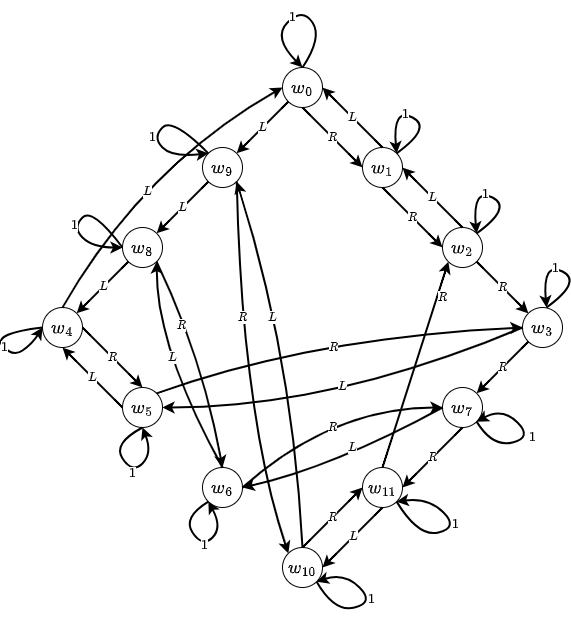
\includegraphics[width=\linewidth]{5BeyondSBDRLGlobalAlgebras/Images/4x1_block_min_actions_wall.png}
    \caption{
    A transition diagram of the labelled transitions in Table \ref{tab:4x1_gridworld_min_transitions_moveable_block}.
    }
    \label{fig:4x1_block_min_actions_wall}
\end{figure}

\begin{fullwidth}
\begin{landscape}
\draftnote{blue}{To do}{
Figure out what to do with this table.
}
\setlength{\tabcolsep}{2pt}
{\fontsize{8}{10}\selectfont
\begin{longtable}[H]{l|lllllllllllllllll}
 & $1$ & $W$ & $E$ & $WW$ & $EW$ & $WE$ & $EE$ & $WWW$ & $EWW$ & $EEW$ & $WWE$ & $WEE$ & $EEE$ & $WWWW$ & $EWWW$ & $EEWW$ & $WEEW$ \\
\midrule
\endfirsthead
 & $1$ & $W$ & $E$ & $WW$ & $EW$ & $WE$ & $EE$ & $WWW$ & $EWW$ & $EEW$ & $WWE$ & $WEE$ & $EEE$ & $WWWW$ & $EWWW$ & $EEWW$ & $WEEW$ \\
\midrule
\endhead
\midrule
\multicolumn{18}{r}{Continued on next page} \\
\midrule
\endfoot
\endlastfoot
\textbf{$1$} & $1$ & $W$ & $E$ & $WW$ & $EW$ & $WE$ & $EE$ & $WWW$ & $EWW$ & $EEW$ & $WWE$ & $WEE$ & $EEE$ & $WWWW$ & $EWWW$ & $EEWW$ & $WEEW$ \\
\textbf{$W$} & $W$ & $WW$ & $WE$ & $WWW$ & $W$ & $WWE$ & $WEE$ & $WWWW$ & $WW$ & $WEEW$ & $WW$ & $WWWW$ & $EWWW$ & $WWE$ & $WWW$ & $EWW$ & $WWE$ \\
\textbf{$E$} & $E$ & $EW$ & $EE$ & $EWW$ & $EEW$ & $E$ & $EEE$ & $EWWW$ & $EEWW$ & $EE$ & $WEEW$ & $EE$ & $EEWW$ & $WEE$ & $EEE$ & $EEW$ & $EEW$ \\
\textbf{$WW$} & $WW$ & $WWW$ & $WWE$ & $WWWW$ & $WW$ & $WW$ & $WWWW$ & $WWE$ & $WWW$ & $WWE$ & $WWW$ & $WWE$ & $WWW$ & $WW$ & $WWWW$ & $WW$ & $WW$ \\
\textbf{$EW$} & $EW$ & $EWW$ & $E$ & $EWWW$ & $EW$ & $WEEW$ & $EE$ & $WEE$ & $EWW$ & $EEW$ & $EWW$ & $WEE$ & $EEE$ & $WEEW$ & $EWWW$ & $EEWW$ & $WEEW$ \\
\textbf{$WE$} & $WE$ & $W$ & $WEE$ & $WW$ & $WEEW$ & $WE$ & $EWWW$ & $WWW$ & $EWW$ & $WEE$ & $WWE$ & $WEE$ & $EWW$ & $WWWW$ & $EWWW$ & $WEEW$ & $WEEW$ \\
\textbf{$EE$} & $EE$ & $EEW$ & $EEE$ & $EEWW$ & $EE$ & $EE$ & $EEWW$ & $EEE$ & $EEW$ & $EEE$ & $EEW$ & $EEE$ & $EEW$ & $EE$ & $EEWW$ & $EE$ & $EE$ \\
\textbf{$WWW$} & $WWW$ & $WWWW$ & $WW$ & $WWE$ & $WWW$ & $WWW$ & $WWE$ & $WW$ & $WWWW$ & $WW$ & $WWWW$ & $WW$ & $WWWW$ & $WWW$ & $WWE$ & $WWW$ & $WWW$ \\
\textbf{$EWW$} & $EWW$ & $EWWW$ & $WEEW$ & $WEE$ & $EWW$ & $EWW$ & $WEE$ & $WEEW$ & $EWWW$ & $WEEW$ & $EWWW$ & $WEEW$ & $EWWW$ & $EWW$ & $WEE$ & $EWW$ & $EWW$ \\
\textbf{$EEW$} & $EEW$ & $EEWW$ & $EE$ & $EEE$ & $EEW$ & $EEW$ & $EEE$ & $EE$ & $EEWW$ & $EE$ & $EEWW$ & $EE$ & $EEWW$ & $EEW$ & $EEE$ & $EEW$ & $EEW$ \\
\textbf{$WWE$} & $WWE$ & $WW$ & $WWWW$ & $WWW$ & $WWE$ & $WWE$ & $WWW$ & $WWWW$ & $WW$ & $WWWW$ & $WW$ & $WWWW$ & $WW$ & $WWE$ & $WWW$ & $WWE$ & $WWE$ \\
\textbf{$WEE$} & $WEE$ & $WEEW$ & $EWWW$ & $EWW$ & $WEE$ & $WEE$ & $EWW$ & $EWWW$ & $WEEW$ & $EWWW$ & $WEEW$ & $EWWW$ & $WEEW$ & $WEE$ & $EWW$ & $WEE$ & $WEE$ \\
\textbf{$EEE$} & $EEE$ & $EE$ & $EEWW$ & $EEW$ & $EEE$ & $EEE$ & $EEW$ & $EEWW$ & $EE$ & $EEWW$ & $EE$ & $EEWW$ & $EE$ & $EEE$ & $EEW$ & $EEE$ & $EEE$ \\
\textbf{$WWWW$} & $WWWW$ & $WWE$ & $WWW$ & $WW$ & $WWWW$ & $WWWW$ & $WW$ & $WWW$ & $WWE$ & $WWW$ & $WWE$ & $WWW$ & $WWE$ & $WWWW$ & $WW$ & $WWWW$ & $WWWW$ \\
\textbf{$EWWW$} & $EWWW$ & $WEE$ & $EWW$ & $WEEW$ & $EWWW$ & $EWWW$ & $WEEW$ & $EWW$ & $WEE$ & $EWW$ & $WEE$ & $EWW$ & $WEE$ & $EWWW$ & $WEEW$ & $EWWW$ & $EWWW$ \\
\textbf{$EEWW$} & $EEWW$ & $EEE$ & $EEW$ & $EE$ & $EEWW$ & $EEWW$ & $EE$ & $EEW$ & $EEE$ & $EEW$ & $EEE$ & $EEW$ & $EEE$ & $EEWW$ & $EE$ & $EEWW$ & $EEWW$ \\
\textbf{$WEEW$} & $WEEW$ & $EWW$ & $WEE$ & $EWWW$ & $WEEW$ & $WEEW$ & $EWWW$ & $WEE$ & $EWW$ & $WEE$ & $EWW$ & $WEE$ & $EWW$ & $WEEW$ & $EWWW$ & $WEEW$ & $WEEW$ \\
\caption{
Cayley table for $\mathscr{W}_{\gamma}$.
}
\end{longtable}

}
\setlength{\tabcolsep}{6pt}
\end{landscape}
\end{fullwidth}


\begin{table}[H]
    \centering
    \begin{tabular}{lc}
    \hline
        \textbf{World} & \bm{$|\hat{A}^{*}/\sim|$} \\
        \hline
        $\mathscr{W}_{\gamma}$ & 17 \\
    \end{tabular}
    \caption{
    The number of elements in the transformation algebra of the world $\mathscr{W}_{\gamma}$.
    \draftnote{blue}{To do}{Redo caption.}
    }
\end{table}

\begin{table}[H]
    \centering
    \begin{tabular}{cc}
        \hline
        \textbf{Property}   & \textbf{Present?} \\
        \hline
        Total               & Y\\
        Associative         & Y\\
        Identity            & Y\\
        Inverse             & N\\
        \hline
        Commutative         & N
    \end{tabular}
    \caption{
    Properties of the $\hat{A}^{*}/\sim$ algebra for the world $\mathscr{W}_{\gamma}$.
    }
\end{table}

\draftnote{blue}{Consider}{
Give agents a letter $\mathscr{A}_{1}$, $\mathscr{A}_{2}$ etc... ? and make sure we mention the algebras as the 
}

%%%%%%%%%%%%%%%%%%%%%%%%%%%%%%%%%%%%%%%%%%%%%
\section{World with irreversible actions}

%%%%%%%%%%%%%%%%%%%%%%%%%%%%%%%%%%%%%%%%%%%%%
\subsection{
An example world \texorpdfstring{$\mathscr{W}_{\zeta}$}{}
}

Consider a world $\mathscr{W}_{\zeta}$ consisting of a $4 \times 1$ cyclical grid containing an agent with minimum actions $\hat{A} = \{1, N, S, E, W, C\}$ and a consumable; if the agent is in the same position as the consumable, the agent can consume the consumable using the consume action $C$.

\begin{figure}[H]
  \centering
  \begin{subfigure}{0.48\textwidth}
    \centering
    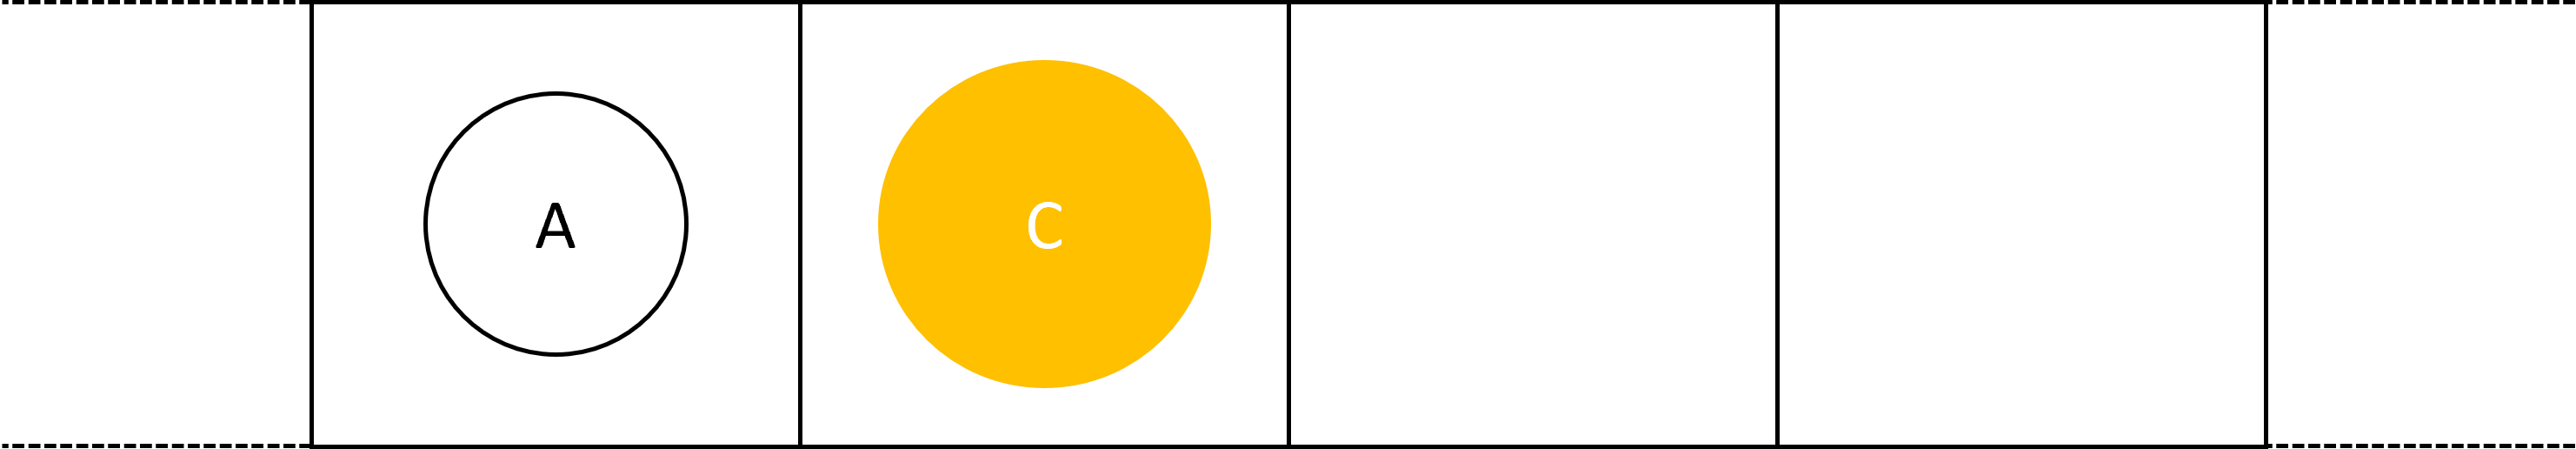
\includegraphics[width=\textwidth]{5BeyondSBDRLGlobalAlgebras/Images/Consumable_world_states/w0.png}
    \caption{$w_{0}$}
    \label{fig:w0}
  \end{subfigure}%
  \hfill
  \begin{subfigure}{0.48\textwidth}
    \centering
    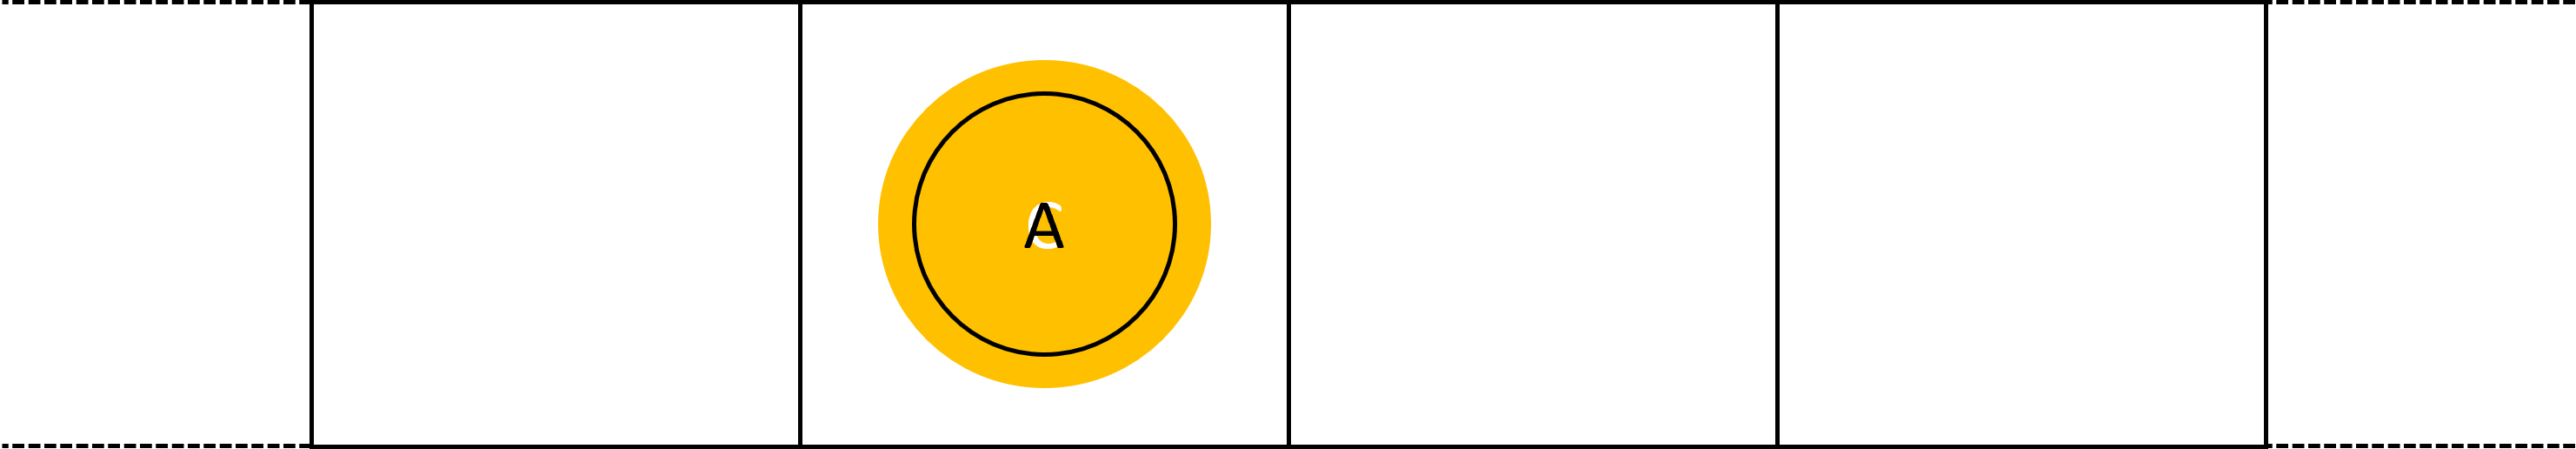
\includegraphics[width=\textwidth]{5BeyondSBDRLGlobalAlgebras/Images/Consumable_world_states/w1.png}
    \caption{$w_{1}$}
    \label{fig:w1}
  \end{subfigure}%
  \vspace{0.5cm}
  \begin{subfigure}{0.48\textwidth}
    \centering
    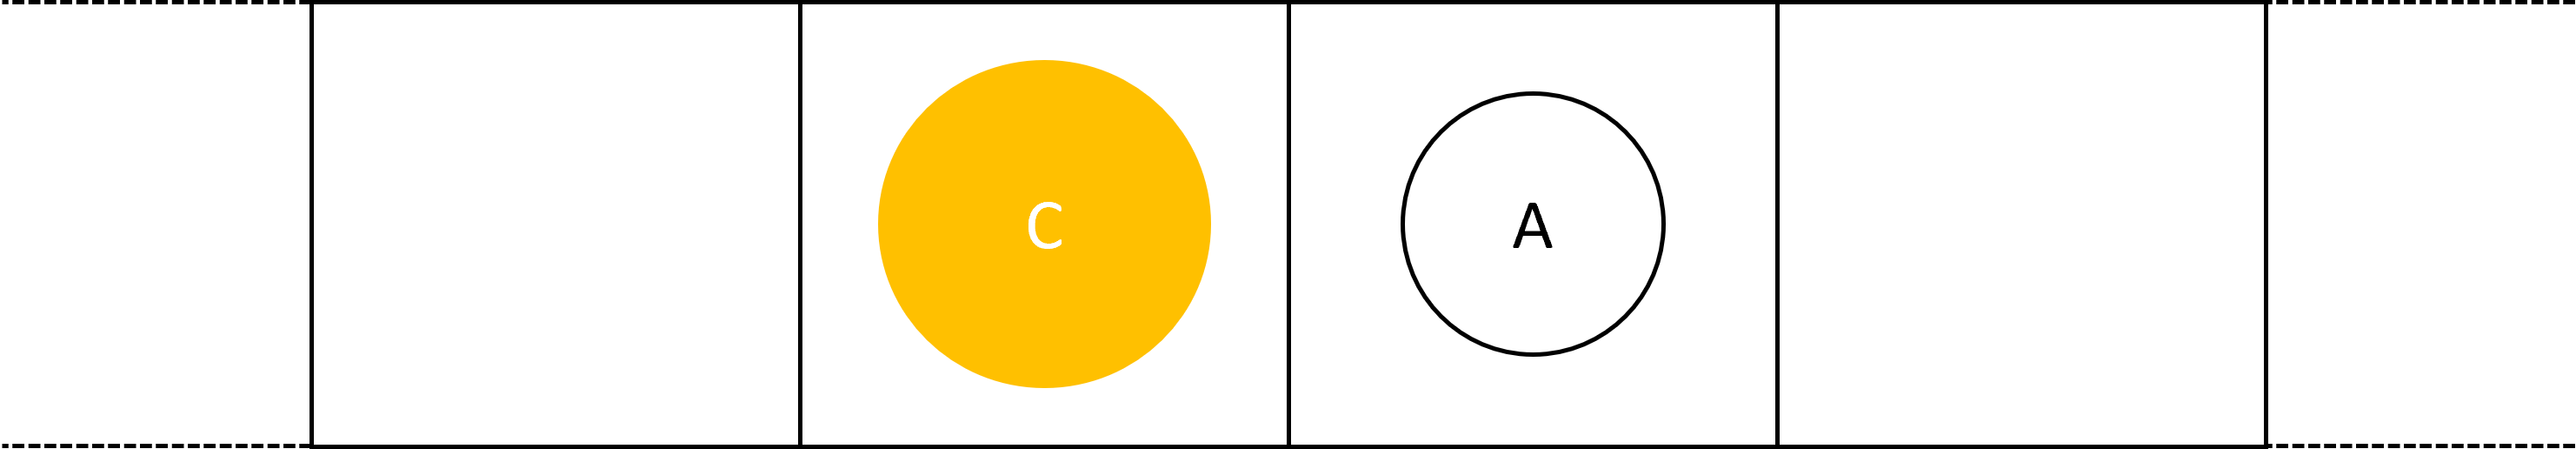
\includegraphics[width=\textwidth]{5BeyondSBDRLGlobalAlgebras/Images/Consumable_world_states/w2.png}
    \caption{$w_{2}$}
    \label{fig:w2}
  \end{subfigure}%
  \hfill
  \begin{subfigure}{0.48\textwidth}
    \centering
    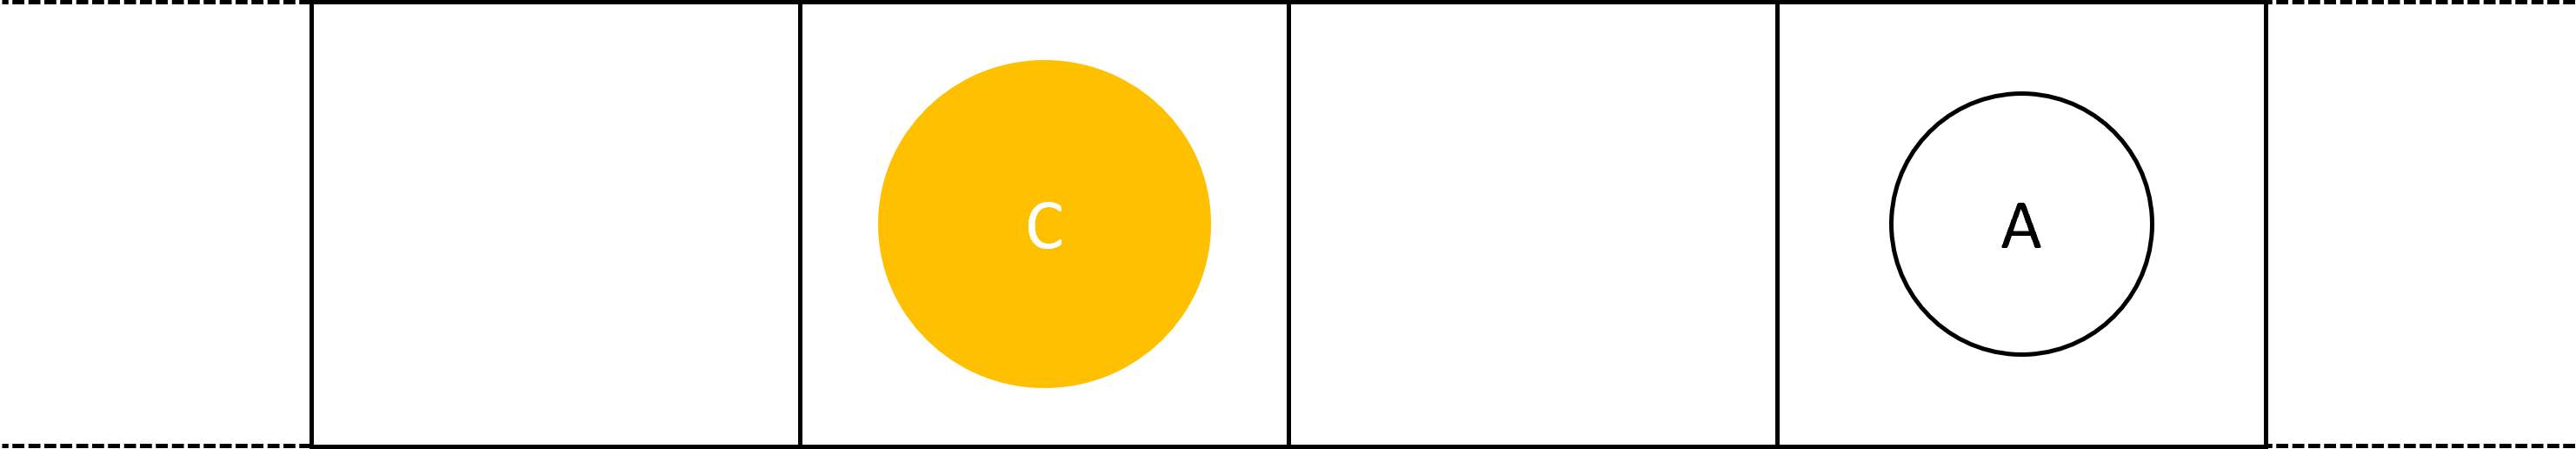
\includegraphics[width=\textwidth]{5BeyondSBDRLGlobalAlgebras/Images/Consumable_world_states/w3.png}
    \caption{$w_{3}$}
    \label{fig:w3}
  \end{subfigure}%
  \vspace{0.5cm}
  \begin{subfigure}{0.48\textwidth}
    \centering
    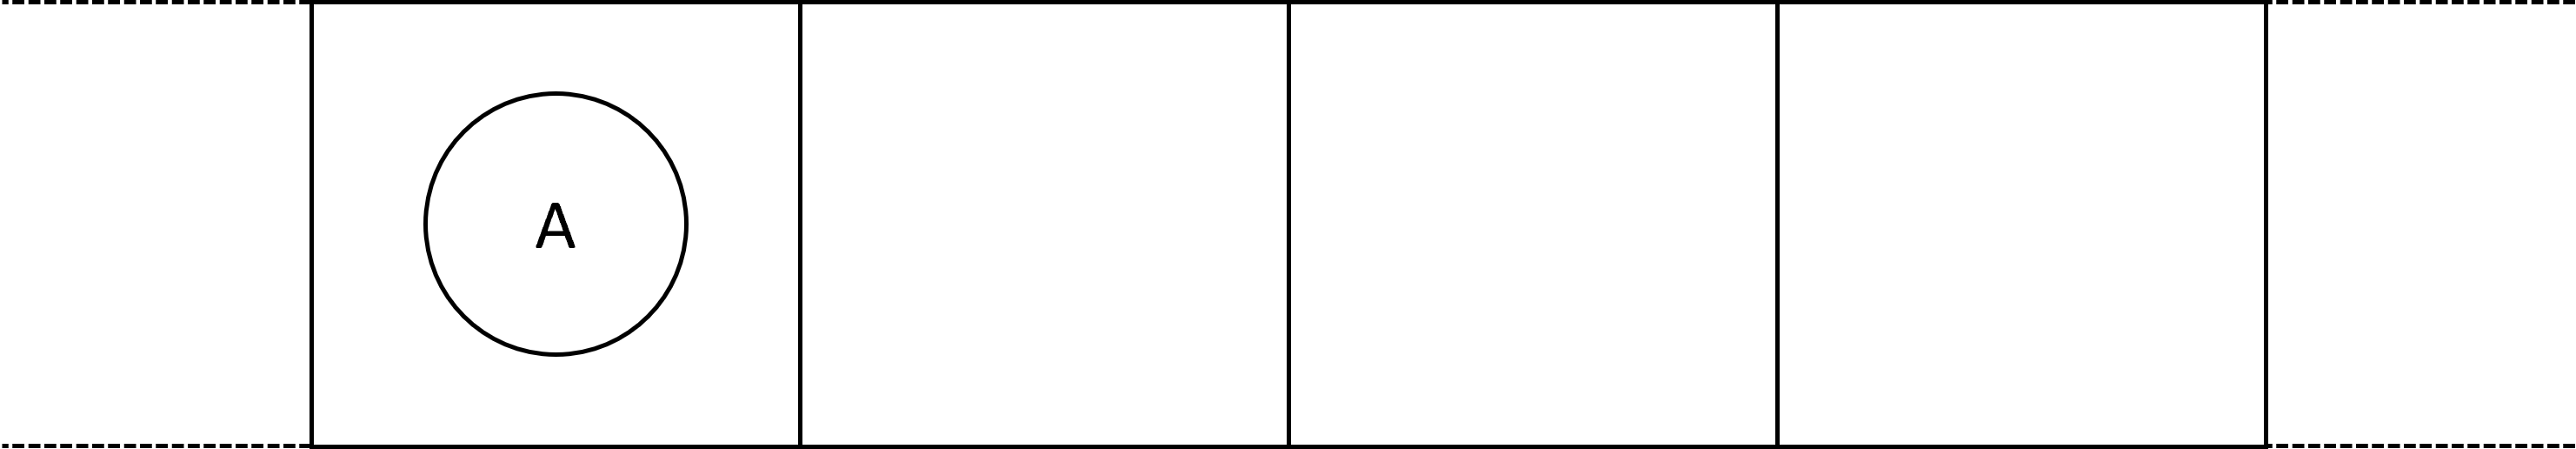
\includegraphics[width=\textwidth]{5BeyondSBDRLGlobalAlgebras/Images/Consumable_world_states/w4.png}
    \caption{$w_{4}$}
    \label{fig:w4}
  \end{subfigure}%
  \hfill
  \begin{subfigure}{0.48\textwidth}
    \centering
    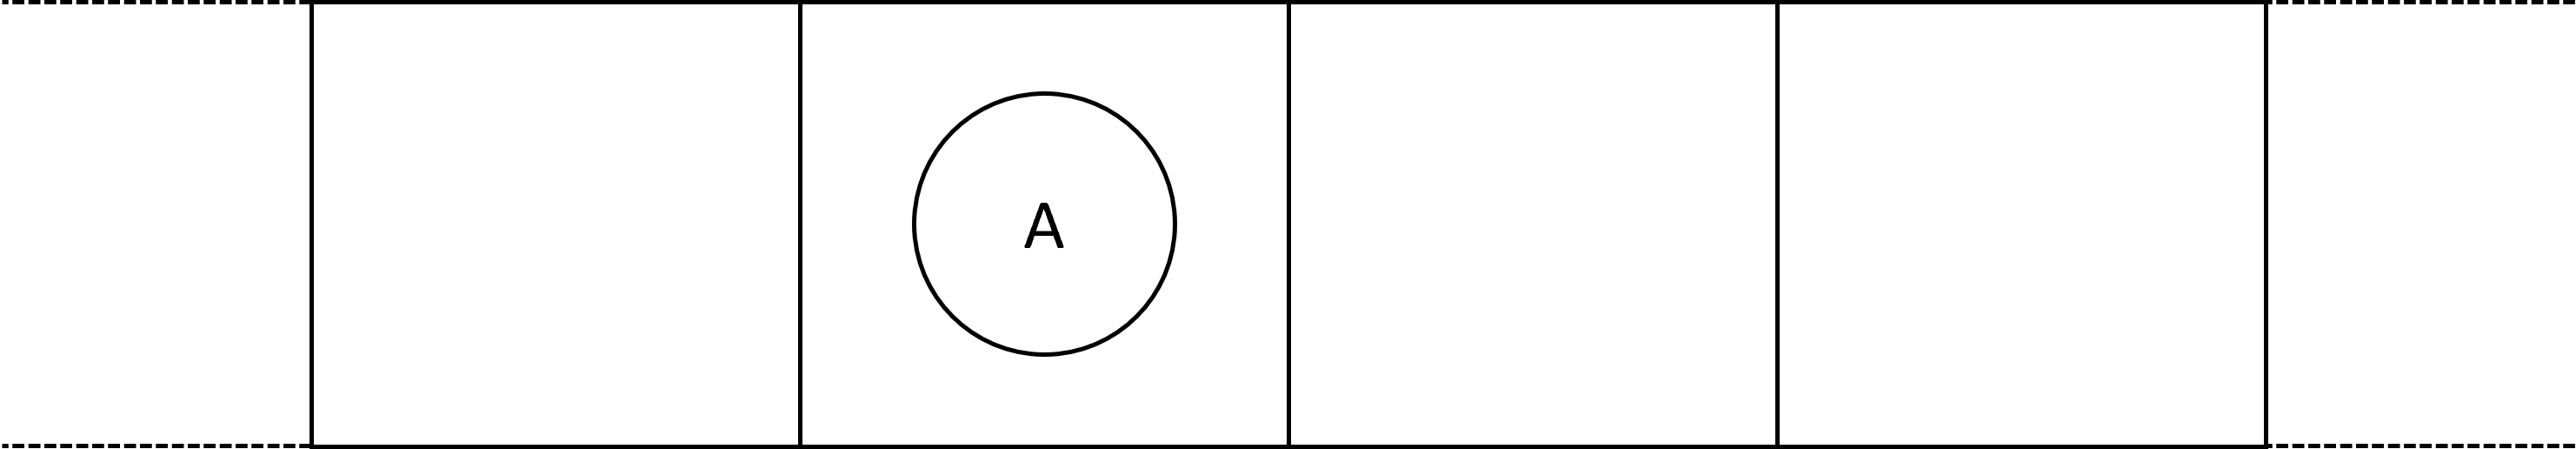
\includegraphics[width=\textwidth]{5BeyondSBDRLGlobalAlgebras/Images/Consumable_world_states/w5.png}
    \caption{$w_{5}$}
    \label{fig:w5}
  \end{subfigure}%
  \vspace{0.5cm}
  \begin{subfigure}{0.48\textwidth}
    \centering
    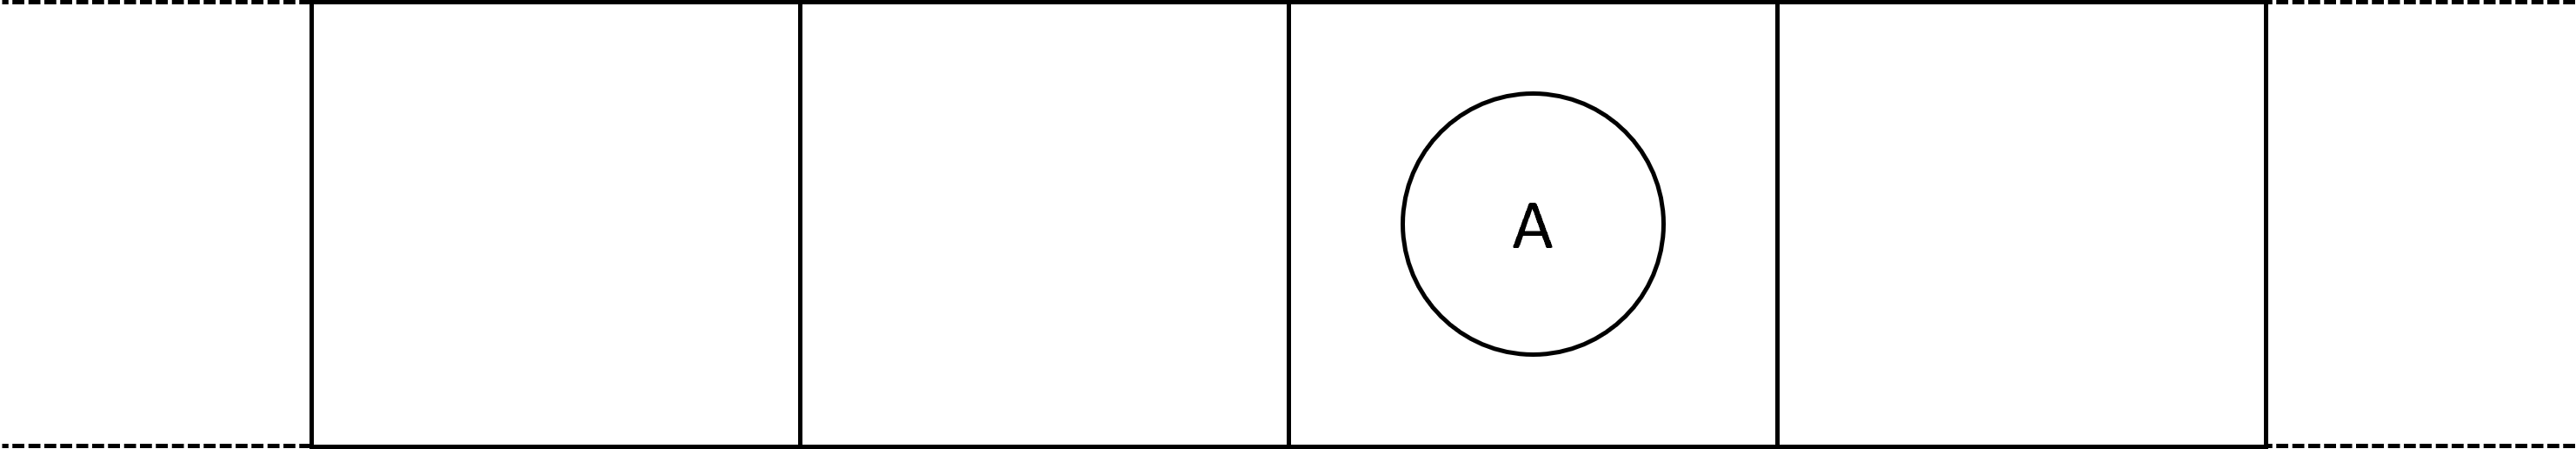
\includegraphics[width=\textwidth]{5BeyondSBDRLGlobalAlgebras/Images/Consumable_world_states/w6.png}
    \caption{$w_{6}$}
    \label{fig:w6}
  \end{subfigure}%
  \hfill
  \begin{subfigure}{0.48\textwidth}
    \centering
    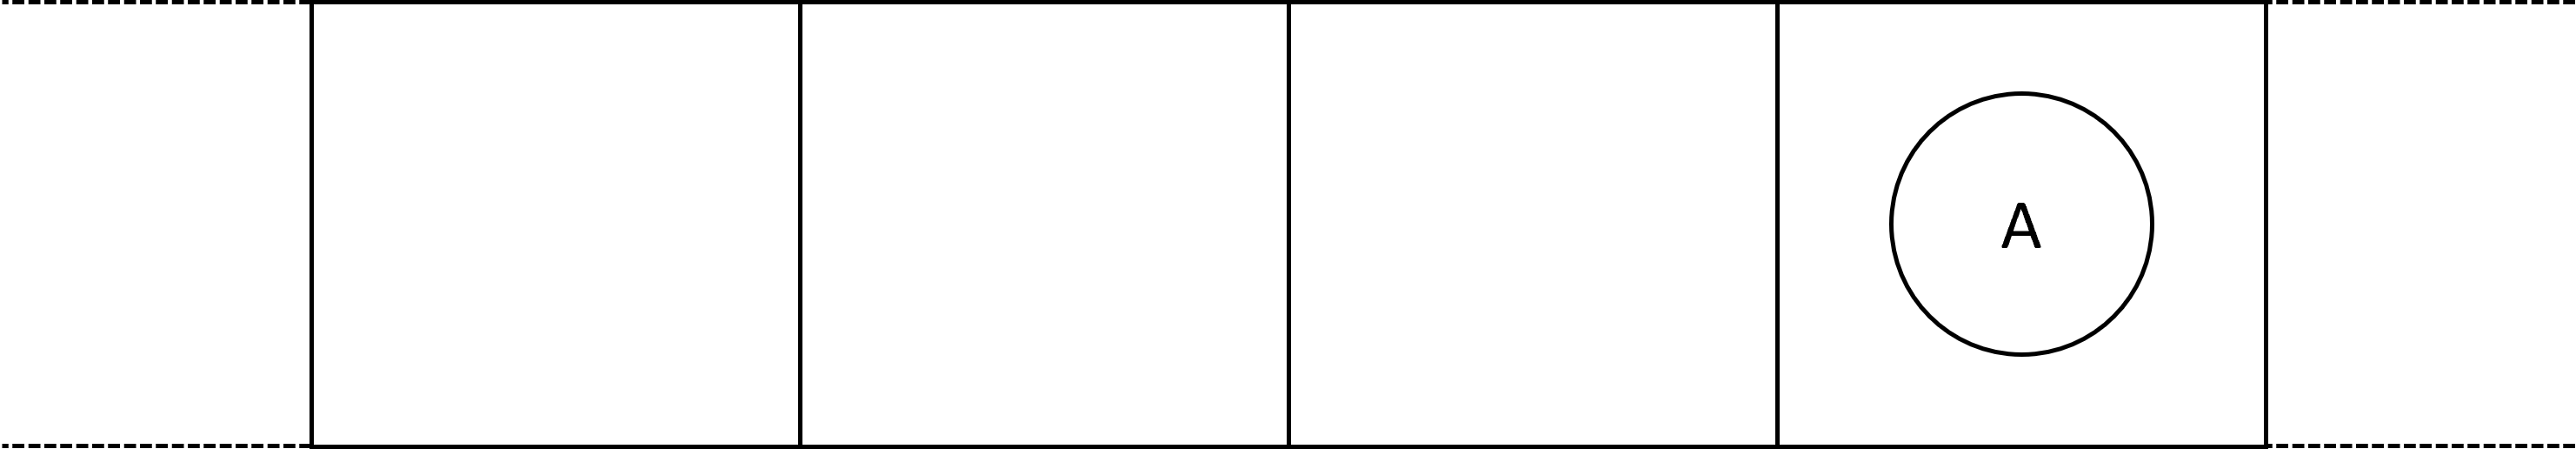
\includegraphics[width=\textwidth]{5BeyondSBDRLGlobalAlgebras/Images/Consumable_world_states/w7.png}
    \caption{$w_{7}$}
    \label{fig:w7}
  \end{subfigure}%
  
  \caption{
  World states of the world $\mathscr{W}_{\zeta}$ containing an agent and a consumable.
  }
  \label{fig:4x1_consumable_world_states}
\end{figure}

The agent is only in the same position as the consumable in world state $w_{1}$, therefore the $C$ action is constrained when $\mathscr{W}_{\gamma}$ is not in $w_{1}$; this means we need to chose a treatment for the consume action $C$ when the world is in a world state $w_{i \neq 1}$.
In this section we will consider the identity treatment of constrained actions in $\mathscr{W}_{\zeta}$\footnote{
We will consider the masked treatment of $\mathscr{W}_{\zeta}$ in \cref{sec:Undefined actions}.
}, so the agent performing the consume action $C$ in a world state $w_{i \neq 1}$ produces the same effect as the agent performing the no op action $1$ (see \cref{fig:min_actions_world_with_consumable_identity}).

\begin{figure}[H]
    \centering
    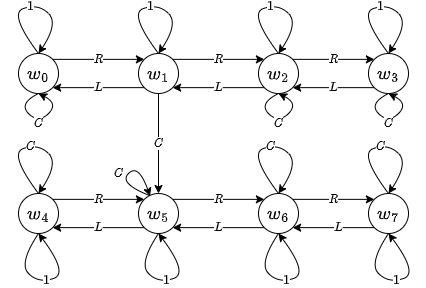
\includegraphics[width=\linewidth]{5BeyondSBDRLGlobalAlgebras/Images/min_actions_world_with_consumable_identity.png}
    \caption{
   World diagram for world $\mathscr{W}_{consumable}$ containing...
    }
    \label{fig:min_actions_world_with_consumable_identity}
\end{figure}

\draftnote{blue}{To do}{
Put Cayley table in appendix.
}

\begin{table}[H]
    \centering
    \begin{tabular}{lc}
    \hline
        \textbf{World} & \bm{$|\hat{A}^{*}/\sim|$} \\
        \hline
        $\mathscr{W}_{\zeta}$ with identity treatment & 64 \\
    \end{tabular}
    \caption{
    The number of elements in the transformation algebra of the world $\mathscr{W}_{\zeta}$ with the identity treatment of constrained actions.
    }
\end{table}

\begin{table}[H]
    \centering
    \begin{tabular}{cc}
        \hline
        \textbf{Property}   & \textbf{Present?} \\
        \hline
        Total               & Y\\
        Associative         & Y\\
        Identity            & Y\\
        Inverse             & N\\
        \hline
        Commutative         & N
    \end{tabular}
    \caption{
    Properties of the $\hat{A}^{*}/\sim$ algebra for the world $\mathscr{W}_{\zeta}$.
    }
\end{table}


%%%%%%%%%%%%%%%%%%%%%%%%%%%%%%%%%%%%%%%%%%%%%
\subsection{
Irreversible actions
}
\draftnote{blue}{Consider}{
\begin{enumerate}
    \item The reachable subworld is preserved by the isomorphism in category theory viewpoint.
    \item Planes of reversibility - see Notion.
    \item "irreversible from a state" vs "irreversible action from a state" ?
\end{enumerate}
}

\draftnote{blue}{awjdean}{
What about transformations that "disappear" when they are used (i.e., next time the same action is performed in that world state the action is constrained) - then we say that the transformation is irreversible and took us to a new world state, so this case is not possible.
Put this as a footnote after doing the world transformation thing to convert $\sim_{t}$ into $\sim$ - same we can use the same trick to deal with problems like the above.
}

For an action $a \in \hat{A}^{*}$ that is irreversible from any state $w \in W$,
\begin{equation}
    \operatorname{Im}(f_{a}) \subsetneq W
\end{equation}
since $w \not\in \operatorname{Im}(f_{a})$ by the definition of $a$ being irreversible from state $w$\footnote{
It is also possible to have $\operatorname{Im}(f_{a}) \subsetneq W$ for reversible actions.
\draftnote{blue}{Include}{
$\mathscr{W}_{\beta}$ with identity treatment example in Notion.
Is $W' = W$ for homogeneous reversible actions? Yes I think so because homogeneous reversible actions are bijections (check this).
}
}.

\draftnote{blue}{Consider}{
Have we said anything about transformations $d: w \xrightarrow{[a]} w'$ ?
$d \in D_{A}/\sim$ or $d \in D_{A/\sim}$ or something similar ?
}

\begin{propositionE}
\label{prp:reachable_subworld_reversible_action}
    \draftnote{blue}{Consider}{
    Move this to Reversible worlds section ?
    }
    If an action $a \in \hat{A}^{*}$ is reversible from $w$, then    \footnote{
    In other words, $\mathscr{W}^{\hat{A}\to}(a \ast w)$ and $\mathscr{W}^{\hat{A}\to}(w)$ coincide, rather than are just isomorphic.
    }
    \begin{equation}
        \mathscr{W}^{\hat{A}\to}(a \ast w) = \mathscr{W}^{\hat{A}\to}(w)
    \end{equation}
\end{propositionE}
\begin{proofE}
\begin{enumerate}
    \item \textbf{Set up.}
    There exists a transformation $d_{1} \in D_{A}$ such that $d_{1}: w \xrightarrow{a} a \ast w$.
    If $a$ is reversible from $w$, then there exists a transformation $d_{2} \in D_{A}$ such that $d_{2}: a \ast w \xrightarrow{a_{2}} w$ where $a_{2} \in \hat{A}^{*}$.
    
    \item \textbf{Show $W^{\hat{A}\to}(w) \subseteq W^{\hat{A}\to}(a \ast w)$.}
    Take any $x \in W^{\hat{A}\to}(w)$.
    From the definition of $W^{\hat{A}\to}(w)$, there exists a transformation $d_{3} \in D_{A}$ such that $d_{3}: w \xrightarrow{a_{3}} x$ where $a_{3} \in \hat{A}^{*}$.
    Therefore, we have a transformation $(d_{3} \circ d_{2}) \in D_{A}$ such that $(d_{3} \circ d_{2}): a \ast w \ \xrightarrow{a_{2}} w \xrightarrow{a_{3}} x$, and so $x \in W^{\hat{A}\to}(a \ast w)$.
    As the choice of $x$ is arbitrary, every world state reachable from $w$ is also reachable from $a \ast w$, and so
    \begin{equation}
        W^{\hat{A}\to}(w) \subseteq W^{\hat{A}\to}(a \ast w)
        \label{eqn:reachable_subworld_w_subset_reachable_subworld_result_reversible}
    \end{equation}

    \item \textbf{Show $W^{\hat{A}\to}(a \ast w) \subseteq W^{\hat{A}\to}(w)$.}
    Take any $y \in W^{\hat{A}\to}(a \ast w)$.
    From the definition of $W^{\hat{A}\to}(a \ast w)$, there exists a transformation $d_{4} \in D_{A}$ such that $d_{4}: a \ast w \xrightarrow{a_{4}} y$ where $a_{4} \in \hat{A}^{*}$.
    Therefore, we have a transformation $(d_{4} \circ d_{1}) \in D_{A}$ such that $(d_{4} \circ d_{1}): w \xrightarrow{a} a \ast w \xrightarrow{a_{4}} y$, and so $y \in W^{\hat{A}\to}(w)$.
    As the choice of $y$ is arbitrary, every world state reachable from $a \ast w$ is also reachable from $w$, and so
    \begin{equation}
        W^{\hat{A}\to}(a \ast w) \subseteq W^{\hat{A}\to}(w)
        \label{eqn:reachable_subworld_result_subset_reachable_subworld_w_reversible}
    \end{equation}

    \item \textbf{Combine results.}
    Combining \cref{eqn:reachable_subworld_w_subset_reachable_subworld_result_reversible,eqn:reachable_subworld_result_subset_reachable_subworld_w_reversible} we have
    \begin{equation}
        W^{\hat{A}\to}(a \ast w) = W^{\hat{A}\to}(w)
    \end{equation}
    From the definition of reachable subworld, the set of reachable world states $W^{\hat{A}\to}(w)$ determines the minimum transformations included in $\hat{D}_{A}^{\hat{A}\to}(w)$ because the set $\hat{D}_{A}^{\hat{A}\to}(w)$ is entirely defined in terms of the source and targets of the minimum action transformations in $\hat{D}_{A}^{\hat{A}\to}(w)$ being in $W^{\hat{A}\to}(w)$, and so if the sets of states coincide, the corresponding collections of minimum transformations also coincide.
    Therefore,
    \begin{equation}
        \mathscr{W}^{\hat{A}\to}(a \ast w) = \mathscr{W}^{\hat{A}\to}(w)
    \end{equation}
\end{enumerate}
\end{proofE}

\begin{propositionE}
\label{prp:reachable_subworld_irreversible_action}
    If an action $a \in \hat{A}^{*}$ is irreversible from $w$, then
    \begin{equation}
        \mathscr{W}^{\hat{A}\to}(a \ast w) \subsetneq \mathscr{W}^{\hat{A}\to}(w)
    \end{equation}
    where
    \begin{equation}
        W^{\hat{A}\to}(a \ast w) \subseteq W \setminus \{w\}
    \end{equation}
    \footnote{
    The reachable subworld $\mathscr{W}^{\hat{A}\to}(a \ast w)$ produced by performing an irreversible action is an induced subgraph of the reachable subworld $\mathscr{W}^{\hat{A}\to}(w)$ because the reachable subworld $\mathscr{W}^{\hat{A}\to}(w)$ preserves all the edges among the world states that remain as the reachable subworld shrinks.
    }
\end{propositionE}
\begin{proofE}
\begin{enumerate}
    \item \textbf{Set up.}
    Since $a$ is irreversible from $w$, by definition there is no transformation $d \in D_{A}$ with $d: a \ast w \xrightarrow{a'} w$ where $a' \in \hat{A}/\sim$.

    \item \textbf{Loss of $w$.}
    In the reachable subworld $\mathscr{W}^{\hat{A}\to}(w)$, $w$ is reachable from itself via the transformation $1_{w}: w \to w$, and so $w \in \mathscr{W}^{\hat{A}\to}(w)$.
    
    Since there is no $d: a \ast w \xrightarrow{a'} w$, by the definition of $W^{\hat{A}\to}(a \ast w)$ it follows that\footnote{
    \textbf{Potential loss of other world states.}
    Consider $x \in W^{\hat{A}\to}(w)$.
    If all transformations $d_{1} \in D_{A}$ such that $a \ast w \to x$ pass through $w$, then when $w$ becomes unreachable $x$ also becomes unreachable.
    \draftnote{blue}{Consider}{
    Can we use $\operatorname{Seq}$ here to make this better ?
    }
    \draftnote{blue}{Footnote?}{
    In subgraph topology, if $w$ is a \emph{hub} or a \emph{bridge} on all possible routes from $w$ to $x$, then when $w$ becomes unreachable $x$ also becomes unreachable.
    }
    }
    \begin{equation}
        w \not\in W^{\hat{A}\to}(a \ast w)
        \label{eqn:w_not_in_reachable_subworld_irreversible}
    \end{equation}
    Therefore,
    \begin{equation}
        W^{\hat{A}\to}(a \ast w) \subseteq W \setminus \{w\}
    \end{equation}

    \item \textbf{Conclusion.}
    From the definition of reachable subworld, the set of reachable world states $W^{\hat{A}\to}(w)$ determines the minimum transformations included in $\hat{D}_{A}^{\hat{A}\to}(w)$ because the set $\hat{D}_{A}^{\hat{A}\to}(w)$ is entirely defined in terms of the source and targets of the minimum action transformations in $\hat{D}_{A}^{\hat{A}\to}(w)$ being in $W^{\hat{A}\to}(w)$.
    
    Therefore, from \cref{eqn:w_not_in_reachable_subworld_irreversible} and the definition of a subworld,
    \begin{equation}
        \mathscr{W}^{\hat{A}\to}(a \ast w) \subsetneq \mathscr{W}^{\hat{A}\to}(w)
    \end{equation}
\end{enumerate}
\end{proofE}



\begin{propositionE}
    For a world $\mathscr{W}$ with transformations only due to the actions of an agent, $|W^{\hat{A}\to}(w^{*})|$ is monotonically non-increasing over time.
\end{propositionE}
\begin{proofE}
\begin{enumerate}
    \item \textbf{Set up.}
    As time proceeds, the world transforms through a sequence of world states as the agent performs actions.
    An action $a \in \hat{A}^{*}/\sim$ can either be (1) reversible, or (2) irreversible from a world state $w \in W$.
    
    \item \textbf{Reversible action.}
    If $a$ is reversible from world state $w^{*}$, then from \cref{prp:reachable_subworld_reversible_action} we have
    \begin{equation}
        W^{\hat{A}\to}(a \ast w^{*}) = W^{\hat{A}\to}(w^{*})
    \end{equation}
    Therefore
    \begin{equation}
        |W^{\hat{A}\to}(a \ast w^{*})| = |W^{\hat{A}\to}(w^{*})|
    \end{equation}
    and so, $|W^{\hat{A}\to}(a \ast w^{*})|$ is unchanged.

    \item \textbf{Irreversible action.}
    If $a$ is irreversible from world state $w^{*}$, then from \cref{prp:reachable_subworld_irreversible_action} we have
    \begin{equation}
        W^{\hat{A}\to}(a \ast w^{*}) \subsetneq W^{\hat{A}\to}(w^{*})
    \end{equation}
    Therefore
    \begin{equation}
        |W^{\hat{A}\to}(a \ast w^{*})| < |W^{\hat{A}\to}(w^{*})|
    \end{equation}
    and so, $|W^{\hat{A}\to}(a \ast w^{*})|$ decreases.
\end{enumerate}
\end{proofE}




\draftnote{blue}{Consider}{
Since $W^{\hat{A}\to}(w^{*})$ decreases monotonically with time, (if actions are performed with some non-zero random distribution) we eventually tend towards the world being reversible (i.e., we tend towards an island of reversibility).
}

%%%%%%%%%%%%%%%%%%%%%%%%%%%%%%%%%%%%%%%%%%%%%
\section{
Undefined actions
}\label{sec:Undefined actions}

\draftnote{green}{To do}{
\begin{enumerate}
    \item Reversible worlds with undefined actions.
    \begin{itemize}
        \item This is the only one which requires care I think since undefined reversible actions act like defined irreversible actions when using the $\bot$ treatment.
    \end{itemize}
    \item Worlds with irreversible actions and worlds with undefined and irreversible actions are structurally the same using the $\bot$ treatment.
\end{enumerate}
}

%%%%%%%%%%%%%%%%%%%%%%%%%%%%%%%%%%%%%%%%%%%%%
\subsection{An example world: irreversible and undefined actions}

$\mathscr{W}_{\gamma}$ with masked treatment is an example of a world with irreversible actions and undefined actions.
Since $C$ is a constrained action when $\mathscr{W}_{\gamma}$ is not in world state $w_{1}$, in the masked treatment when $\mathscr{W}_{\gamma}$ is in world state $w_{i \neq 1}$ we say the $C$ action is undefined.
The world states of $\mathscr{W}_{\gamma}$ are given in \cref{fig:4x1_consumable_world_states}.

\begin{figure}[H]
    \centering
    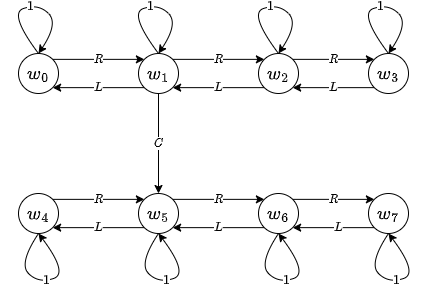
\includegraphics[width=\linewidth]{5BeyondSBDRLGlobalAlgebras/Images/min_actions_world_with_consumable_masked.png}
    \caption{
    \draftnote{blue}{To do}{Redo caption.}
    Minimum action network for world containing an agent and a consumable.
    }
\end{figure}

\draftnote{blue}{To do}{
Put Cayley table in appendix.
}

\begin{table}[H]
    \centering
    \begin{tabular}{lc}
    \hline
        \textbf{World} & \bm{$|\hat{A}^{*}/\sim|$} \\
        \hline
        $\mathscr{W}_{\zeta}$ with masked treatment & 21 \\
    \end{tabular}
    \caption{
    \draftnote{blue}{awjdean}{
    Old method give $|\hat{A}^{*}/\sim| = 20$, action functions method gives $|\hat{A}^{*}/\sim| = 21$.
    Check - find differences and figure out which equivalence classes they're in.
    }
    The number of elements in the transformation algebra of the world $\mathscr{W}_{\zeta}$ with the masked treatment of constrained actions.
    }
\end{table}

\begin{table}[H]
    \centering
    \begin{tabular}{cc}
        \hline
        \textbf{Property}   & \textbf{Present?} \\
        \hline
        Total               & N\\
        Associative         & Y\\
        Identity            & Y\\
        Inverse             & N\\
        \hline
        Commutative         & N
    \end{tabular}
    \caption{
    Properties of the $\hat{A}^{*}/\sim$ algebra for the world $\mathscr{W}_{\zeta}$ with the masked treatment of constrained actions.
    }
\end{table}


%%%%%%%%%%%%%%%%%%%%%%%%%%%%%%%%%%%%%%%%%%%%%
\subsection{
Two perspectives
}

\draftnote{blue}{To do}{
Does my algorithm give any situation with masked actions as non reversible ?
Change how property check is done so it's "when defined" ?
}

There are two perspectives we can consider when a world-agent pair has undefined actions
\begin{enumerate}
    \item $(\hat{A}^{*}/\sim, \circ_{\sim})$ is a monoid with a partially defined action $\ast: \hat{A}^{*}/\sim \times W \rightharpoonup W$, where $\ast$ is undefined if there is no corresponding transformation in $D_{A}$; or
    \item $(\hat{A}^{*}/\sim, \circ_{\sim})$ is a small category with a total action $\ast: \hat{A}^{*}/\sim \times W \to W$.
\end{enumerate}

When we augment our system with the undefined state $\bot$, the operator $\ast_{\sim}^{\bot}: \hat{A}^{*}/\sim \times W^{\bot} \to W^{\bot}$ is partial or total based on whether we decide to allow $\bot$ as a legitimate image or we ignore the $\bot$ state.

\draftnote{blue}{Consider}{
Mention something about the first perspective being favoured in category theory, and the second being favoured in monoid theory.
}

%%%%%%%%%%%%%%%%%%%%%%%%%%%%%%%%%%%%%%%%%%%%%
\subsection{
(?) Reversible and undefined actions
}

\draftnote{green}{Include}{
\begin{enumerate}
    \item Cases where groupoid is not a group action ?
    \begin{itemize}
        \item This might depend on action homogeneity.
    \end{itemize}
    \item Does my algorithm give any situation with masked actions as non reversible ?
\end{enumerate}
}
